\documentclass{report}
\usepackage{nth}
\usepackage{amsmath}
\usepackage{fancyhdr}
\pagestyle{fancy}
\usepackage{titlesec}
\usepackage{amsmath}
\usepackage{amssymb}
\usepackage{graphicx}
\usepackage{csquotes}
\usepackage{pgfplots}
\pgfplotsset{compat=1.18}
\usepackage{hyperref}
\usepackage{listings}
\usepackage{algorithm}
\usepackage{algpseudocode}
\usepackage{multicol}
\usepackage[italian]{babel}
\usepackage[a4paper, margin=2cm]{geometry}
\usepackage{tcolorbox}
\usepackage{subcaption}

\fancyhead[L]{Metodi di Ritrovamento delle Informazioni}
\fancyhead[R]{Marco Ferrara}

\setlength{\headheight}{15pt}

\title{MRI - Metodi di Ritrovamento delle Informazioni}
\author{Marco Ferrara}
\date{Ottobre 2024}

\begin{document}
	\maketitle
	\tableofcontents
	\newpage
	
	\chapter{Document/Text Mining: From Text to Knowledge}
	\section{Introduzione}
	La gestione della conoscenza è un processo strategico che consiste nel raccogliere, organizzare, distribuire e rendere facilmente accessibile l'informazione all'interno di un'organizzazione o di un sistema. Questo approccio mira a far sì che le persone possano accedere rapidamente alle informazioni di cui hanno bisogno, nel momento e nel luogo più appropriato, con l'obiettivo di risparmiare tempo, migliorare la qualità dei servizi offerti e ridurre i tempi di accesso all'informazione.

	Uno degli aspetti chiave della gestione della conoscenza è la modalità con cui le informazioni vengono ricercate e rese disponibili. La ricerca attiva avviene quando l'utente richiede specificamente un'informazione o un servizio e riceve una risposta mirata. Al contrario, la ricerca passiva si verifica quando un sistema intelligente propone informazioni rilevanti all'utente anche senza una richiesta esplicita, anticipando i suoi bisogni. Questa capacità di fornire informazioni proattivamente può migliorare significativamente l'efficienza operativa e la qualità delle decisioni.
	
	La conoscenza, soprattutto in contesti aziendali e organizzativi, è un capitale intangibile, difficile da concretizzare e conservare. Essa è altamente volatile, poiché dipende spesso da fattori umani come l'esperienza e il know-how, che possono andare persi quando un individuo lascia un'organizzazione o non documenta adeguatamente le sue competenze. Per questo motivo, gestire correttamente la conoscenza è cruciale per preservare e trasferire il sapere all'interno dell'organizzazione, evitando perdite di valore.
	
	Una sfida particolare nella gestione della conoscenza è rappresentata dai dati non strutturati, che costituiscono circa il 90\% del patrimonio informativo di un'organizzazione. I dati non strutturati includono documenti in formato testuale, email, messaggi, relazioni, immagini e contenuti multimediali, che non seguono uno schema rigido come i dati strutturati, conservati in database organizzati. Poiché la maggior parte delle informazioni utili risiede in questi dati non strutturati, diventa fondamentale disporre di strumenti in grado di processarli e renderli fruibili.
	
	L'obiettivo principale della gestione della conoscenza, quindi, è sviluppare sistemi capaci di comprendere e processare documenti in linguaggio naturale, acquisendo e recuperando informazioni rilevanti da basi di dati testuali o non strutturati. Questo processo è reso possibile attraverso tecniche avanzate come la classificazione dei documenti, che permette di categorizzare automaticamente le informazioni; l'estrazione delle informazioni, che identifica e isola dati significativi all'interno di testi complessi; e il text mining, che analizza grandi volumi di dati per scoprire pattern, tendenze e relazioni nascoste. 
	
	Implementare con successo queste tecnologie consente di trasformare il caos dei dati non strutturati in risorse preziose, migliorando la capacità decisionale, l'innovazione e l'efficienza complessiva di un'organizzazione. Inoltre, sistemi avanzati di gestione della conoscenza possono offrire un vantaggio competitivo, permettendo un accesso rapido e preciso alle informazioni strategiche che guidano il successo aziendale.
	
	\section{Search vs Discover}
	\begin{center}
		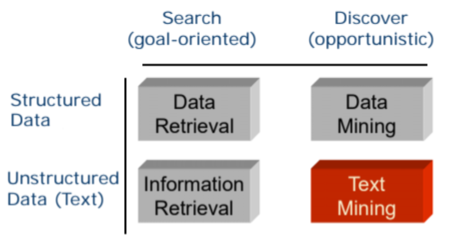
\includegraphics[scale=0.6]{assets/searchvsdiscover.png}
	\end{center}
	La figura illustra le differenze tra i due approcci principali nella gestione e ricerca delle informazioni: la \textbf{Search} (ricerca) e la \textbf{Discover} (scoperta). Questi due approcci si collegano alla natura dei dati, che possono essere \textbf{strutturati} o \textbf{non strutturati}.

	\begin{itemize}
    \item \textbf{Search (goal-oriented)}: 
    Questo approccio è orientato a un obiettivo specifico, con una ricerca attiva da parte dell'utente per ottenere risposte precise. Si applica sia a dati strutturati, come i database, sia a dati non strutturati, come testi o documenti.
    \begin{itemize}
        \item Per i \textbf{dati strutturati}, si usa il termine \textbf{Data Retrieval}, ovvero il recupero di dati specifici da un database tramite query SQL, ad esempio.
        \item Per i \textbf{dati non strutturati}, si parla di \textbf{Information Retrieval}, ovvero la ricerca in grandi quantità di testo per trovare documenti o informazioni rilevanti tramite parole chiave o query.
    \end{itemize}

    \item \textbf{Discover (opportunistic)}:
    Questo approccio è più passivo e opportunistico. L'utente non cerca informazioni specifiche, ma lascia che il sistema identifichi per lui dati rilevanti, anche se non richiesti esplicitamente.
    	\begin{itemize}
        	\item Per i \textbf{dati strutturati}, si utilizza il \textbf{Data Mining}, una tecnica che permette di analizzare grandi volumi di dati per identificare pattern nascosti, tendenze o relazioni all'interno di un database ben organizzato.
        	\item Per i \textbf{dati non strutturati}, viene applicato il \textbf{Text Mining}, evidenziato in rosso nella figura. Questa tecnica si occupa di estrarre informazioni significative da grandi quantità di testo, come articoli, documenti o messaggi. L'obiettivo è scoprire relazioni nascoste o conoscenze latenti, che non emergono con una semplice ricerca per parole chiave.
    	\end{itemize}
	\end{itemize}

	\subsection{Data Retrieval}
	Il \textbf{Data Retrieval} è il processo di recupero di dati specifici da un database strutturato, come un database relazionale. Questo approccio è utilizzato per trovare informazioni precise in risposta a una query formulata dall'utente. 
	\begin{center}
		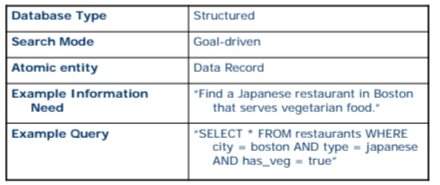
\includegraphics[scale=0.6]{assets/dataretrieval.png}
	\end{center}

	\subsection{Information Retrieval}
	L'\textbf{Information Retrieval} è il processo di ricerca di informazioni rilevanti all'interno di grandi quantità di testo o documenti non strutturati. Questo approccio è utilizzato per trovare documenti o informazioni pertinenti in risposta a una query formulata dall'utente.
	\begin{center}
		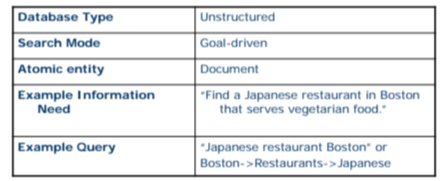
\includegraphics[scale=0.6]{assets/inforetrieval.png}
	\end{center}

	\subsection{Data Mining}
	Il \textbf{Data Mining} è una tecnica che permette di analizzare grandi volumi di dati strutturati per identificare pattern nascosti, tendenze o relazioni all'interno di un database ben organizzato. Questo approccio è utilizzato per scoprire informazioni significative e conoscenze latenti che non emergono con una semplice analisi dei dati. Il punto focale è l'assenza di una query specifica da parte dell'utente.
	\begin{center}
		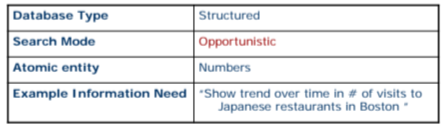
\includegraphics[scale=0.6]{assets/datamining.png}
	\end{center}

	\subsection{Il Processo di KDD (Knowledge Discovery from Databases)}
	La scoperta di conoscenza nei database (\textbf{KDD}) è definita come "il processo non banale di identificazione di pattern validi, nuovi, potenzialmente utili e comprensibili nei dati".
	\vspace{\baselineskip}\\
	Il processo di KDD è composto da diverse fasi, come mostrato nello schema. In particolare, il \textbf{data mining} rappresenta solo uno degli step intermedi di questo processo, anche se è comunemente confuso con l'intero processo di KDD.

	\begin{itemize}
    	\item \textbf{Selezione dei dati}: In questa prima fase, vengono selezionati i dati 	rilevanti da una fonte più ampia.
    	\item \textbf{Pre-processing}: I dati vengono poi pre-processati, per rimuovere rumori o valori mancanti, e prepararli per l'analisi successiva.
    	\item \textbf{Trasformazione}: I dati pre-processati vengono trasformati in un formato che possa essere utilizzato più facilmente per il data mining. Ad esempio, la riduzione della dimensionalità o l'aggregazione di alcune caratteristiche può avvenire in questa fase.
    	\item \textbf{Data Mining}: Questa fase centrale consiste nell'applicare tecniche di data mining per estrarre pattern utili e interessanti dai dati. Questo passo è solo una parte del processo generale.
   		\item \textbf{Interpretazione/Valutazione}: Una volta identificati i pattern, essi vengono interpretati e valutati per determinare se sono validi, utili e comprensibili. Da questa fase finale emerge la conoscenza che può essere utilizzata nei vari contesti applicativi.
	\end{itemize}
	\begin{center}
		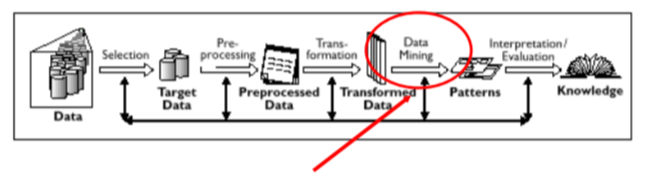
\includegraphics[scale=0.6]{assets/kdd.png}
	\end{center}

	\subsection{DataMining @ Work}
	\begin{center}
		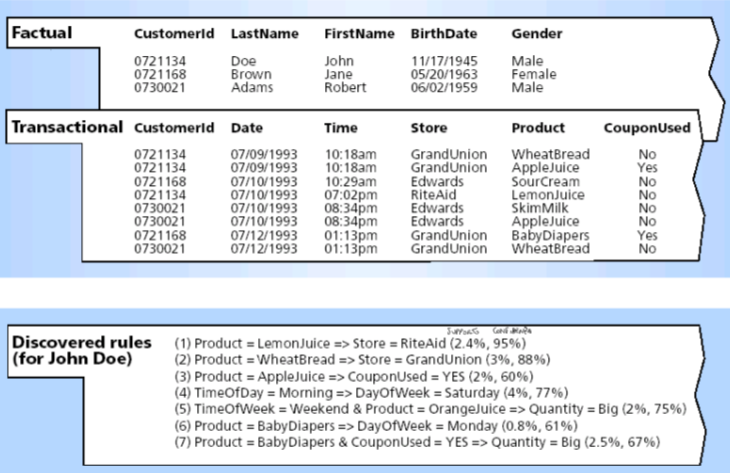
\includegraphics[scale=0.6]{assets/dataminingwork.png}
	\end{center}
	I dati mostrati nell'immagine sono suddivisi in due categorie principali:
	\begin{itemize}
    	\item \textbf{Dati fattuali}: informazioni anagrafiche di ciascun cliente come \textit{CustomerId}, \textit{LastName} (cognome), \textit{FirstName} (nome), \textit{BirthDate} (data di nascita), e \textit{Gender} (genere).
    	\item \textbf{Dati transazionali}: dati che registrano ogni transazione con informazioni quali \textit{CustomerId}, \textit{Date} (data della transazione), \textit{Time} (orario), \textit{Store} (negozio), \textit{Product} (prodotto acquistato), e se è stato utilizzato un \textit{Coupon}.
	\end{itemize}

	Le \textbf{regole di associazione} sono tecniche utilizzate per identificare relazioni e pattern nei dati. Si basano sull'analisi di transazioni per trovare prodotti che tendono a essere acquistati insieme o eventi che si verificano frequentemente in determinati contesti. Nell'immagine, sono mostrate regole di associazione relative al cliente \textit{John Doe}.
	\vspace{\baselineskip}\\
	Il \textbf{supporto} misura la frequenza con cui un pattern appare nel dataset complessivo. Si calcola come la frazione di transazioni che contengono gli itemset di interesse rispetto al numero totale di transazioni. Formalmente:
	\[
		\text{Supporto}(A \Rightarrow B) = \frac{\text{Numero di transazioni che contengono } A \text{ e } B}{\text{Numero totale di transazioni}}
	\]
    \vspace{\baselineskip}\\
	La \textbf{confidenza} misura quanto è probabile che la parte destra della regola si verifichi quando la parte sinistra è vera. In altre parole, rappresenta la probabilità condizionata che $B$ sia presente nelle transazioni che contengono $A$. Formalmente:
	\[
		\text{Confidenza}(A \Rightarrow B) = \frac{\text{Supporto}(A \cup B)}{\text{Supporto}(A)}
	\]

	Ecco alcune regole di associazione presenti nell'immagine:
	\begin{itemize}
    	\item \textbf{(1) "Product = LemonJuice} $\Rightarrow$ \textbf{Store = RiteAid (2.4\%, 95\%)"}: Questa regola significa che quando viene acquistato del succo di limone, la transazione avviene nel negozio "RiteAid" nel 2.4\% delle transazioni, con un livello di \textit{confidenza} del 95\%.
    	\begin{itemize}
        	\item \textbf{Supporto (2.4\%)}: La percentuale di transazioni in cui questa associazione (prodotto = LemonJuice e negozio = RiteAid) si verifica sul totale delle transazioni.
        	\item \textbf{Confidenza (95\%)}: Percentuale di volte in cui, dato che è stato acquistato il succo di limone, la transazione avviene effettivamente nel negozio RiteAid.
    	\end{itemize}
		\item \textbf{(3) Product = AppleJuice $\Rightarrow$ CouponUsed = YES (2\%, 60\%)}: Il succo di mela viene acquistato e viene usato un coupon nel 2\% delle transazioni, con una probabilità del 60\% di uso del coupon quando viene acquistato il succo di mela.
		\item \textbf{(5) TimeOfWeek = Weekend \& Product = OrangeJuice $\Rightarrow$ Quantity = Big (2\%, 75\%)}: Durante il fine settimana, se viene acquistato succo d'arancia, nel 75\% dei casi la quantità acquistata è grande.
	\end{itemize}

	\subsection{Text Mining}
	Il \textbf{Text Mining} è una tecnica che si occupa di  estrarre informazioni utili da grandi volumi di dati testuali, evidenziando un processo non banale. In questo contesto, "non banale" significa che le informazioni estratte non sono immediatamente evidenti o già conosciute. Il processo consiste nello scoprire modelli, tendenze e intuizioni che possono essere utili ma che sono nascoste all'interno del testo. Il Text Mining è fondamentalmente l'applicazione di tecniche di Data Mining ai dati testuali, arricchita da una conoscenza di base della linguistica. L'obiettivo è rivelare informazioni implicite, precedentemente sconosciute e potenzialmente utili che si trovano nascoste in grandi quantità di testi.

	\begin{center}
		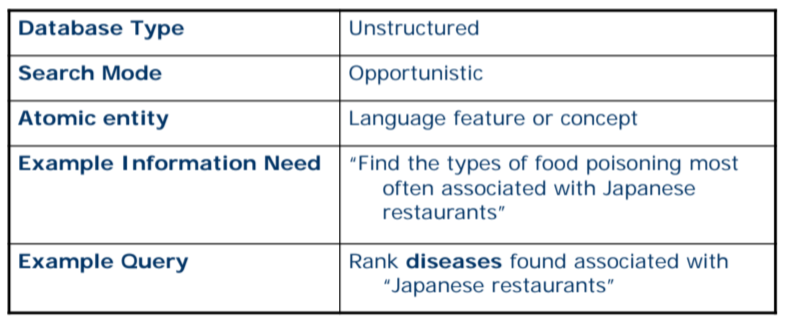
\includegraphics[scale=0.5]{assets/textmining.png}
	\end{center}
	Come il data mining, il text mining è un processo iterativo che coinvolge diverse fasi:
	\begin{itemize}
		\item \textbf{Text Pre-processing}: In questa fase, i testi vengono analizzati dal punto di vista sintattico e semantico per rimuovere errori e rumori, normalizzare i dati e prepararli per l'analisi successiva.
		\item \textbf{Feature Generation}: I testi vengono trasformati in una rappresentazione numerica, ad esempio attraverso la creazione di vettori di parole o l'uso di tecniche di embedding (Bag of words) che estraggono parole chiave o concetti rilevanti modellandoli in insiemi non ordinati.
		\item \textbf{Feature Selection}: In questa fase, vengono selezionate le caratteristiche più rilevanti per l'analisi, riducendo la dimensionalità dei dati e migliorando l'efficienza computazionale. In questa fase vengono effettuate statistiche descrittive e analisi esplorative dei dati.
		\item \textbf{Text/Data Mining}: Questa fase centrale consiste nell'applicare tecniche di text mining o data mining per estrarre pattern, tendenze o relazioni nascoste nei dati testuali. Le tecniche possono essere supervisionate come la classificazione o non supervisionate come il clustering.
		\item \textbf{Evaluation}: Una volta identificati i pattern, essi vengono valutati per determinare la loro validità, utilità e comprensibilità. Questa fase è cruciale per garantire che le informazioni estratte siano affidabili e significative.
	\end{itemize}
	\begin{center}
		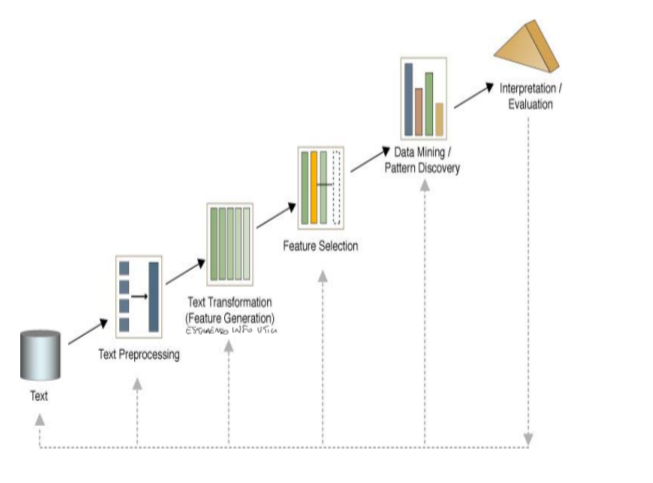
\includegraphics[scale=0.6]{assets/textminingprocess.png}
	\end{center}

	\subsection{Text Mining @ Work}
	\begin{center}
		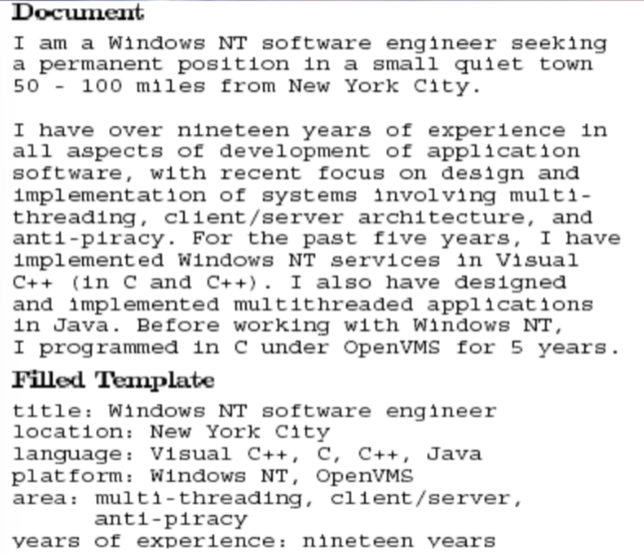
\includegraphics[scale=0.6]{assets/textminingwork.png}
	\end{center}
	Questo esempio mostra l'applicazione del Text Mining su un documento di testo non strutturato, che descrive le competenze e l'esperienza di un ingegnere software. Il testo originale contiene dettagli come il tipo di posizione cercata, la località, gli anni di esperienza e le competenze tecniche. A partire da questo testo, attraverso il processo di Text Mining, le informazioni vengono estratte e organizzate in un formato strutturato.
	\vspace{\baselineskip}\\
	Questo esempio dimostra come il Text Mining possa essere utilizzato per estrarre automaticamente informazioni rilevanti da testi non strutturati, trasformandoli in dati strutturati, rendendone così più facile la comprensione, la ricerca e l'analisi.
	\vspace{\baselineskip}\\
	In questo specifico esempio, il Text Mining avrebbe aiutato a identificare le competenze e le esperienze chiave dell'ingegnere software, facilitando il processo di selezione e di matching con le posizioni lavorative disponibili con la possibilità di affiancare una AI per scartare automaticamente i CV non in linea con le competenze richieste.

	\subsection{Text Mining nell'Impresa}
	Il Text Mining è utilizzato in una vasta gamma di applicazioni, tra cui l'analisi dei sentimenti, la categorizzazione dei documenti, l'estrazione delle informazioni, la classificazione dei testi e la generazione di sommari automatici. Queste applicazioni sono utili in diversi settori, come il marketing, la finanza, la sanità, l'assistenza clienti e la sicurezza informatica. Il processo di estrazione della conoscenza è utilizzabile durante i processi di Business Intelligence, per l'analisi dei dati e la generazione di report, e per migliorare la qualità delle decisioni aziendali.
	\vspace{\baselineskip}\\
	Il Text Mining in ambito business è \textbf{necessario} per vari motivi:
	\begin{itemize}
		\item permette di scoprire opinioni, idee, tendenze, gusti dei clienti. Operazione sempre più complessa poichè i dati a disposizione sono sempre più numerosi e complessi e i cambi di tendenza sono sempre più rapidi.
		\item permette di semplificare l'analisi di fonti che sono sempre più eterogenee e complesse.
		\item permette di analizzare miliardi di documenti in pochi secondi, raggruppando i documenti in base a temi, argomenti, sentimenti. Processo che sarebbe impossibile da fare manualmente.
	\end{itemize}

	\chapter{Information Retrieval (IR)}
	L'Information Retrieval (IR) si occupa della rappresentazione, archiviazione, organizzazione e accesso agli elementi informativi.
	\vspace{\baselineskip}\\
	Gli elementi informativi possono includere:
	\begin{itemize}
		\item documenti,
		\item pagine Web,
		\item cataloghi online,
		\item record strutturati,
		\item oggetti multimediali.
	\end{itemize}
	Gli obiettivi iniziali dell'area IR erano indicizzare il testo e cercare documenti utili in una collezione. La ricerca di pagine sul World Wide Web è l'applicazione più recente e rilevante in questo campo.
	\vspace{\baselineskip}\\
	L'IR si concentra primariamente sul recupero di documenti \emph{rilevanti} rispetto a una query. Secondariamente, si occupa di recuperare documenti da grandi insiemi di dati in modo \emph{efficiente}.
	\vspace{\baselineskip}\\
	Il processo di recupero dell'informazione parte dalla disponibilità di un insieme di documenti testuali scritti in linguaggio naturale, che costituiscono una collezione di riferimento. All'utente viene richiesto di fornire una query, ossia una stringa di testo che descrive le informazioni di cui ha bisogno. L'obiettivo è quello di individuare un insieme di documenti, ordinati in base alla loro rilevanza, che rispondano in modo soddisfacente alla query inserita dall'utente.
	\vspace{\baselineskip}\\
	Un esempio di necessità informativa complessa potrebbe essere la seguente: trovare tutti i documenti che trattano il ruolo del Governo Federale nel finanziamento delle operazioni della National Railroad Transportation Corporation (AMTRAK).
	\vspace{\baselineskip}\\
	Questa query data dall'utente non deve necessariamente essere una buona query da sottomettere al sistema di IR. L'utente potrebbe voler trasformare le informazioni richieste in una query più specifica e precisa. Questo processo di trasformazione della richiesta dell'utente in una query porta alla formazione di un'insieme di \textbf{keywords}, \textbf{index terms}, che riassumono le informazioni richieste. Questo insieme di termini viene sottomesso al sistema di IR per trovare i documenti rilevanti. L'IR andrà poi a rankare i documenti in base alla loro rilevanza rispetto alla query.
	\begin{center}
		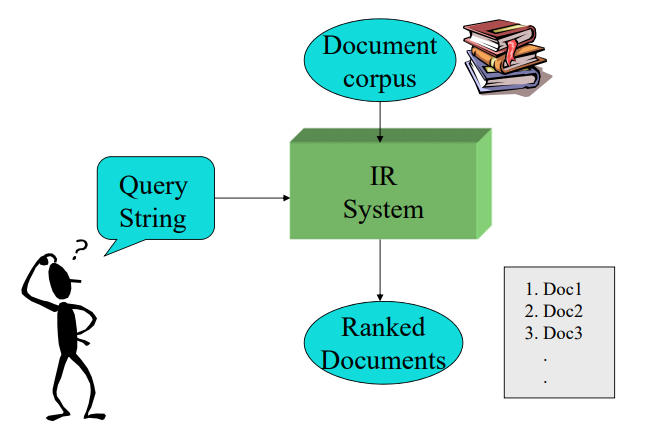
\includegraphics[scale=0.6]{assets/irsystem.png}
	\end{center}

	\section{Come gli utenti cercano informazioni}
	L'interazione degli utenti con le interfacce di ricerca varia significativamente a seconda di diversi fattori chiave. In primo luogo, il tipo di compito influisce in modo decisivo sul modo in cui un utente conduce una ricerca. Ad esempio, la ricerca di una singola informazione è molto diversa da una ricerca esplorativa, che mira a una comprensione più approfondita di un argomento complesso. Anche l'esperienza dell'utente nel dominio di interesse gioca un ruolo fondamentale: un esperto utilizzerà strategie di ricerca più avanzate rispetto a un utente meno esperto. Infine, la quantità di tempo e sforzo che un utente può dedicare al processo di ricerca influisce su come quest'ultimo viene condotto. Ricerche rapide e mirate sono tipiche in condizioni di tempo limitato, mentre ricerche più approfondite richiedono un maggiore impegno e dedizione.
	\vspace{\baselineskip}\\
	Un'importante distinzione nell'ambito della ricerca riguarda la differenza tra \textbf{information lookup} e \textbf{exploratory search}. L'\textbf{information lookup} si riferisce a compiti in cui l'obiettivo è il recupero di fatti o la risposta a domande specifiche. Tali compiti possono essere soddisfatti da pezzi discreti di informazione, come numeri, date, nomi o siti web, e funzionano bene nelle interazioni standard con i motori di ricerca. Ad esempio, cercare su Google la data di nascita di una celebrità o il nome di un prodotto rientra in questa categoria.
	\vspace{\baselineskip}\\
	La \textbf{exploratory search}, al contrario, è un processo più complesso che può essere suddiviso in due tipi principali: la \textbf{learning search} e la ricerca investigativa (\textbf{investigating}). La \textbf{learning search} richiede molto più di una semplice interazione domanda-risposta. In questo caso, l'utente deve investire tempo nel leggere e analizzare diverse fonti di informazione, sintetizzando il contenuto per ottenere una nuova comprensione. Questo tipo di ricerca è tipico nei contesti educativi o quando si vuole acquisire una conoscenza approfondita su un argomento nuovo.
	\vspace{\baselineskip}\\
	La fase di \textbf{investigating} è invece un processo più lungo e iterativo. Può durare nel tempo e comportare numerose iterazioni, durante le quali l'utente valuta criticamente i risultati prima di integrarli nelle proprie conoscenze, sia personali che professionali. Questo tipo di ricerca non mira solo a ottenere una risposta specifica, ma piuttosto a raccogliere una grande quantità di informazioni rilevanti. Esempi di \textbf{investigating} includono ricerche accademiche, studi legali o indagini scientifiche.
	\vspace{\baselineskip}\\
	L'attività di ricerca è spesso inserita in un processo più ampio, chiamato \textbf{sensemaking}, che consiste nel dare un significato coerente e strutturato a una vasta collezione di informazioni. Il \textbf{sensemaking} è un processo iterativo in cui la principale difficoltà risiede nella sintesi di una rappresentazione concettuale chiara e utile a partire da un gran numero di dati. Alcune attività di \textbf{sensemaking} alternano fasi di ricerca e fasi di analisi, mentre altre prevedono un approccio più integrato, dove la ricerca e la sintesi avvengono simultaneamente.
	\vspace{\baselineskip}\\
	Ci sono diversi contesti in cui il \textbf{sensemaking}, oltre alla ricerca, è fondamentale per completare compiti complessi che richiedono un'analisi approfondita. Esempi di tali compiti includono il processo di \textbf{legal discovery}, in cui si devono esaminare grandi quantità di documenti per trovare prove rilevanti; l'epidemiologia, che comporta il monitoraggio delle malattie; lo studio delle lamentele dei clienti per migliorare il servizio; e l'intelligence aziendale, che implica l'analisi di dati complessi per prendere decisioni strategiche.+
	
	\section{Rilevanza}
	Il concetto di \textbf{rilevanza} è intrinsecamente soggettivo e dipende da molteplici fattori. La rilevanza di un documento non è univoca, ma può essere valutata in base a criteri specifici. Tra questi, il documento può essere considerato rilevante se tratta il \textbf{tema appropriato}, se fornisce informazioni \textbf{tempestive} e aggiornate (cioè, recenti), oppure se soddisfa gli obiettivi dell'utente e il suo specifico \textbf{bisogno informativo}. In quest'ultimo caso, la rilevanza è legata all'utilizzo che l'utente intende fare dell'informazione recuperata. 
	\vspace{\baselineskip}\\
	La nozione più semplice di \textbf{rilevanza} si basa sul fatto che la stringa di query appaia esattamente, in forma verbatim, all'interno del documento. Un concetto leggermente meno rigido di rilevanza è quello del modello \textbf{bag of words} (insieme di parole), in cui le parole della query appaiono frequentemente nel documento, anche se in ordine diverso. 
	\vspace{\baselineskip}\\
	Tuttavia, l'uso delle parole chiave può presentare dei problemi. Uno dei principali riguarda il fatto che le parole chiave potrebbero non recuperare documenti rilevanti che includono termini \textbf{sinonimi}. Ad esempio, la parola \textit{“restaurant”} potrebbe non recuperare documenti che usano il termine \textit{“café”}, anche se si riferiscono allo stesso concetto. Allo stesso modo, la parola \textit{“PRC”} potrebbe non recuperare documenti che contengono la parola \textit{“China”}, sebbene entrambi i termini facciano riferimento alla Repubblica Popolare Cinese. 
	\vspace{\baselineskip}\\
	Un altro problema riguarda la possibile presenza di termini \textbf{ambigui} (\textbf{polisemia}), che possono portare a recuperare documenti non pertinenti. Ad esempio, il termine \textit{“bat”} può riferirsi sia a una \textbf{mazza} da baseball, sia a un \textbf{pipistrello} (mammifero). Similmente, la parola \textit{“Apple”} può riferirsi sia all'\textbf{azienda tecnologica} che al \textbf{frutto}, causando potenzialmente il recupero di documenti non rilevanti rispetto alla query dell'utente.

	\section{Architettura di un Sistema di IR}
	\begin{center}
		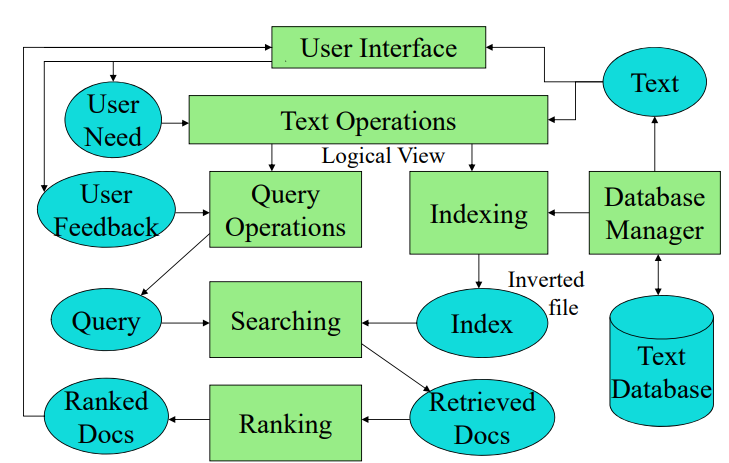
\includegraphics[scale=0.5]{assets/irsystemarch.png}
	\end{center}
	Un sistema di \textbf{Information Retrieval} (IR) è progettato per soddisfare il bisogno informativo di un utente attraverso il recupero di documenti rilevanti da un ampio database testuale. L'immagine presentata rappresenta l'architettura tipica di un sistema IR, in cui i vari moduli lavorano in sinergia per facilitare il processo di ricerca e presentazione dei documenti.
	\vspace{\baselineskip}\\
	L'architettura di un sistema IR comprende i seguenti componenti principali:
	\begin{itemize}
		\item \textbf{User Interface}: L'utente interagisce con il sistema attraverso l'\textbf{interfaccia utente} (\textbf{User Interface}), che permette di inserire le query e visualizzare i risultati. Questa interfaccia funge da tramite tra l'utente e il resto del sistema, traducendo i bisogni informativi dell'utente in query comprensibili dal sistema.
		\item \textbf{User Need e User Feedback}: Il \textbf{bisogno informativo} (\textbf{User Need}) dell'utente rappresenta la motivazione iniziale per l'interrogazione del sistema. Il sistema può anche ricevere \textbf{feedback} dall'utente sui risultati forniti, per raffinare le query future e migliorare la pertinenza dei risultati.
		\item \textbf{Text Operations}: Le \textbf{operazioni testuali} (\textbf{Text Operations}) sono un insieme di processi che preparano i dati testuali per la fase di ricerca. Questi processi includono la rimozione delle parole comuni e non informative (\textit{stopword removal}) e la riduzione delle parole alle loro radici (\textit{stemming}).
		\item \textbf{Indexing e Inverted Index}: L'operazione di \textbf{indicizzazione} (\textbf{Indexing}) costruisce un \textbf{indice invertito} (\textbf{inverted index}) che associa ciascun termine o \textbf{token} ai documenti in cui esso appare. Questo indice rappresenta una mappa da parole a puntatori ai documenti, consentendo un recupero rapido ed efficiente dei documenti che contengono un certo termine.
		\item \textbf{Query Operations}: Le \textbf{operazioni sulla query} (\textbf{Query Operations}) sono responsabili della gestione delle query inserite dagli utenti. Esse includono la trasformazione della query in un formato compatibile con l'indice e la preparazione della query per la ricerca all'interno del database.
		\item \textbf{Searching}: La fase di \textbf{ricerca} (\textbf{Searching}) sfrutta l'indice invertito per individuare i documenti che contengono i termini presenti nella query dell'utente. Una volta recuperati i documenti corrispondenti, questi vengono passati alla fase di classificazione.
		\item \textbf{Ranking}: La fase di \textbf{classificazione} (\textbf{Ranking}) assegna un punteggio di rilevanza a ciascun documento recuperato, basato su una metrica di rilevanza specifica. Questa fase può anche includere la \textbf{raggruppamento} (\textbf{grouping}), che consiste nel trovare somiglianze tra i documenti e presentarli in gruppi per facilitare l'interpretazione da parte dell'utente.
		\item \textbf{Retrieved Docs e Ranked Docs}: Infine, i \textbf{documenti recuperati} (\textbf{Retrieved Docs}) vengono ordinati in base alla rilevanza e presentati all'utente come \textbf{documenti classificati} (\textbf{Ranked Docs}). Questo ordine di classificazione aiuta l'utente a identificare rapidamente i documenti più pertinenti alla sua query.
	\end{itemize}
	Il sistema IR segue un flusso logico di operazioni. Il testo viene inizialmente processato per creare un indice che permette una ricerca efficiente. L'utente inserisce una query attraverso l'interfaccia utente, che viene trasformata e confrontata con l'indice. I documenti corrispondenti vengono recuperati e classificati per rilevanza, e infine presentati all'utente, che può fornire un feedback per migliorare i risultati futuri.

	\section{Natural Language Processing (NLP)}
	Il \textbf{Natural Language Processing} (NLP) è un campo interdisciplinare che combina la linguistica computazionale, l'intelligenza artificiale e l'informatica per consentire ai computer di comprendere, interpretare e generare il linguaggio umano in modo naturale. Si concentra sull'analisi sintattica, semantica e pragmatica dei testi e dei discorsi in linguaggio naturale, al fine di estrarre significato e informazioni utili. E' un processo utile per determinare il senso di una parola ambigua in base al contesto (\textbf{word sense disambiguation}), per identificare specifiche informazioni all'interno di documenti (\textbf{information extraction}), e per rispondere a specifiche domande poste in linguaggio naturale (\textbf{question answering}).
	
	\section{Machine Learning}
	Il \textbf{Machine Learning} (ML) si occupa di sviluppare algoritmi e modelli che consentono ai computer di apprendere automaticamente da dati e di migliorare le proprie prestazioni nel tempo con l'esperienza. Il ML è ampiamente utilizzato nell'ambito dell'IR per migliorare la precisione e l'efficienza dei sistemi di ricerca. Distinguiamo due tipi principali di apprendimento automatico:
	\begin{itemize}
		\item \textbf{Apprendimento Supervisionato}: In questo approccio, il modello viene addestrato su un insieme di dati etichettati, in cui ogni esempio di input è associato a una corrispondente etichetta di output. Il modello apprende a mappare gli input alle etichette attraverso l'analisi dei dati di addestramento. Questo tipo di apprendimento è comunemente utilizzato per la classificazione e la regressione.
		\item \textbf{Apprendimento Non Supervisionato}: In questo approccio, il modello viene addestrato su un insieme di dati non etichettati, senza informazioni sull'output desiderato. Il modello cerca di trovare pattern e struttura nei dati, raggruppando gli esempi in base a somiglianze o differenze. Questo tipo di apprendimento è comunemente utilizzato per il clustering e la riduzione della dimensionalità.
	\end{itemize}

	\section{Modelli di Ritrovamento dell'Informazione}
	Un modello di ritrovamento delle informazioni specifica come i documenti sono rappresentati e confrontati con le query, come le stesse query degli utenti devono essere rappresentate per determinare la rilevanza dei documenti. Il modello determina la metrica di rilevanza che viene utilizzata per classificare i documenti in base alla loro pertinenza rispetto alla query. Questi metriche possono essere di due tipi:
	\begin{itemize}
		\item \textbf{Binarie}: i documenti sono classificati come rilevanti o non rilevanti rispetto alla query senza dare informazioni aggiuntive circa la rilevanza. \\Con questa metrica è impossibile determinare un ranking di rilevanza tra i documenti.
		\item \textbf{Continua}: i documenti sono classificati in base a un punteggio di rilevanza, che può variare da 0 a 1 o da 0 a 100, o in base ad una percentuale di rilevanza. Questa metrica permette di determinare un ranking di rilevanza tra i documenti.
	\end{itemize}

	Un modello IR è una quadrupla $M = (D, Q, F, R(q_i, d_j))$, dove:
	\begin{itemize}
		\item $D$ è l'insieme delle rappresentazioni logiche dei documenti nella collezione,
		\item $Q$ è l'insieme delle rappresentazioni logiche delle query degli utenti,
		\item $F$ è un framework di modellazione dei documenti e delle query,
		\item $R(q_i, d_j)$ è la funzione di ranking di rilevanza che assegna un punteggio di rilevanza tra la query $q_i$ e il documento $d_j$.
	\end{itemize}
	\begin{center}
		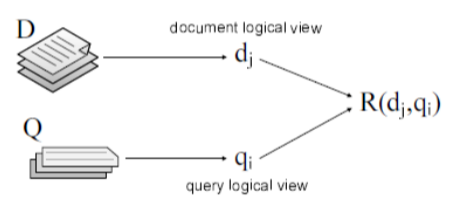
\includegraphics[scale=0.6]{assets/irmodel.png}
	\end{center}
	
	\section{Tassonomia di un Modello IR}
	\begin{center}
		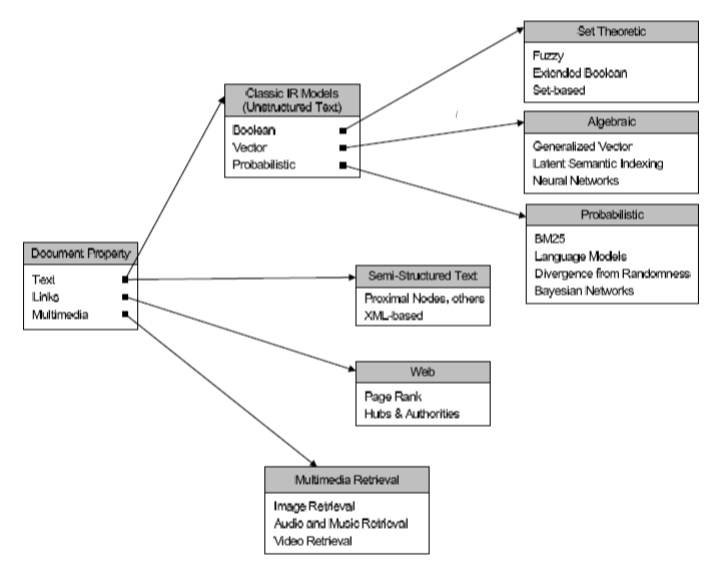
\includegraphics[scale=0.5]{assets/irtaxonomy.png}
	\end{center}
	Un modello di ritrovamento delle informazioni può essere classificato in base a diversi criteri, tra cui il tipo di rappresentazione dei documenti e delle query, il tipo di metrica di rilevanza utilizzata e il tipo di framework di modellazione adottato. La tassonomia di un modello IR che lavorano su testi non strutturati può essere suddivisa in diverse categorie principali, tra cui:
	\begin{itemize}
		\item \textbf{Modelli Booleani (teorici degli insiemi)}: 
		I modelli booleani si basano sulla logica degli insiemi e utilizzano operatori logici (\texttt{AND}, \texttt{OR}, \texttt{NOT}) per determinare la rilevanza di un documento. In questo contesto, un documento può essere considerato rilevante (1) o irrilevante (0) in base alla presenza o assenza di parole chiave specifiche.
		
		Tuttavia, il modello booleano classico ha alcune limitazioni: non tiene conto della frequenza con cui un termine compare nel documento e non permette di classificare i documenti per grado di rilevanza. Per affrontare questi limiti, esiste l'**Extended Boolean Model**, che introduce un approccio più flessibile e può gestire sfumature intermedie di rilevanza.
	
		\item \textbf{Modelli a Spazio Vettoriale (statistici/algebrici)}: 
		Nei modelli a spazio vettoriale, sia i documenti che le query vengono rappresentati come vettori in uno spazio multidimensionale, dove ogni dimensione corrisponde a un termine. La somiglianza tra un documento e una query è determinata in base alla distanza o angolo tra i rispettivi vettori, misurata solitamente tramite il coseno dell'angolo tra essi (\emph{cosine similarity}).
		
		Esistono varianti di questo modello, come:
		\begin{itemize}
			\item \textbf{Generalized Vector Space Model}: Estende il modello vettoriale standard, prendendo in considerazione le correlazioni tra i termini.
			\item \textbf{Latent Semantic Indexing (LSI)}: Questo approccio riduce la dimensionalità dello spazio vettoriale utilizzando tecniche di decomposizione della matrice, identificando relazioni semantiche latenti tra i termini per migliorare il recupero delle informazioni.
		\end{itemize}
	
		\item \textbf{Modelli Probabilistici}: 
		I modelli probabilistici si basano sulla probabilità che un documento sia rilevante rispetto a una query. Invece di trattare i documenti come puramente rilevanti o irrilevanti, come nei modelli booleani, questi modelli considerano la probabilità di rilevanza. Un esempio comune è il modello probabilistico di recupero di base, dove si calcola la probabilità \(P(R=1|D,Q)\) che un documento \(D\) sia rilevante (\(R=1\)) data una query \(Q\).
		
		Questi modelli possono anche considerare fattori come la frequenza delle parole, il che li rende più flessibili rispetto ai modelli booleani. Ciò consente di classificare i documenti in base alla probabilità di rilevanza, migliorando la qualità dei risultati rispetto ai modelli binari.
	\end{itemize}
	
	\section{Processi comuni di Pre-Processing}
	Prima di eseguire operazioni di recupero delle informazioni o elaborazione del linguaggio naturale, i testi devono essere preprocessati per rimuovere elementi non essenziali e facilitare il lavoro dei modelli. Di seguito sono elencati i principali passi di pre-processing comunemente eseguiti:

	\begin{itemize}
		\item \textbf{Rimozione di caratteri non desiderati o markup}: In questa fase vengono eliminati elementi come tag HTML, punteggiatura, numeri e altri caratteri non alfanumerici che potrebbero interferire con l'analisi del testo. Questo passaggio pulisce il testo e lo riduce ai soli contenuti informativi, facilitando l'elaborazione successiva.
		\item \textbf{Tokenizzazione}: Il testo viene suddiviso in \emph{token}, che sono generalmente singole parole o frasi chiave, separati da spazi bianchi. Questo permette di lavorare con singole unità lessicali (parole), facilitando l'analisi delle occorrenze nei documenti.
		\item \textbf{Stemming (riduzione alle radici)}: I token vengono ridotti alle loro "radici" o forme base, rendendo il processo di recupero delle informazioni indipendente da varianti come il tempo verbale o il numero. Ad esempio, "computational" può essere ridotto a "comput". Tuttavia, questo processo può introdurre errori. Ad esempio, parole come "policies" e "police" potrebbero entrambe essere ridotte a "polic", creando ambiguità. Altri problemi includono la perdita di contesto (ad esempio "does" che diventa "do") e la possibilità che la radice ottenuta non sia una parola di senso compiuto.
		\item \textbf{Rimozione delle stopwords}: Le parole molto comuni che non apportano molto significato al contenuto, come "a", "the", "it", vengono rimosse. Queste parole sono chiamate \emph{stopwords} e la loro rimozione aiuta a concentrarsi sui termini più significativi nel testo. L'obiettivo è ridurre il rumore nel testo, rendendo il processo di recupero delle informazioni più efficiente.
		\item \textbf{Rilevamento di frasi comuni}: A volte, le singole parole non catturano il contesto completo. Pertanto, si possono identificare frasi ricorrenti o rilevanti, spesso utilizzando dizionari specifici per il dominio in esame. Questo passaggio aiuta a catturare espressioni idiomatiche o termini tecnici composti che potrebbero essere persi analizzando solo singoli token.
		\item \textbf{Costruzione di un indice invertito}: Dopo la fase di pre-processing, viene costruito un \emph{indice invertito}, che associa ogni parola o token chiave a una lista di documenti che lo contengono. Ad esempio, il termine "keyword" sarà associato a tutti i documenti che contengono quella parola. Questo passaggio è fondamentale per migliorare l'efficienza nel recupero dei documenti pertinenti durante una ricerca, riducendo il tempo necessario per identificare i risultati.
	\end{itemize}

	Queste tecniche di pre-processing migliorano notevolmente la qualità e l'efficacia dei risultati nei sistemi di recupero delle informazioni, riducendo il rumore e rendendo i dati più gestibili.

	\section{Modello Booleano}
	Il \textbf{Modello Booleano} è uno dei primi modelli di recupero delle informazioni sviluppati e si basa sulla logica degli insiemi. In questo modello, i documenti e le query sono rappresentati come insiemi di termini, e la rilevanza di un documento rispetto a una query è determinata utilizzando operatori logici come \texttt{AND}, \texttt{OR} e \texttt{NOT}, comprese parentesi per indicare lo scope. Questi operatori consentono di combinare i termini della query e dei documenti per determinare la loro corrispondenza. Il risultato di una query è la rilevanza binaria di ciascun documento rispetto alla query, che può essere classificata come rilevante (1) o non rilevante (0). Non viene calcolato un ranking di rilevanza tra i documenti e non ci possono essere risultati parziali.

	\subsection{Matrice di Incidenza Documento-Termine}
	Una rappresentazione comune dei documenti e dei termini in un modello booleano è la \textbf{matrice di incidenza documento-termine}. In questa rappresentazione, ogni riga della matrice corrisponde ad una parola chiave o termine, mentre ogni colonna corrisponde a un documento. Gli elementi della matrice indicano se un termine appare o meno in un documento, utilizzando valori binari (1 per presenza, 0 per assenza). Questa rappresentazione consente di confrontare rapidamente e graficamente i documenti con le query utilizzando operatori logici ma non è conveniente con una mole di termini e documenti elevata.

	\paragraph{Esempio}
	Query: Brutus AND Caesar AND NOT Calpurnia
	\begin{center}
		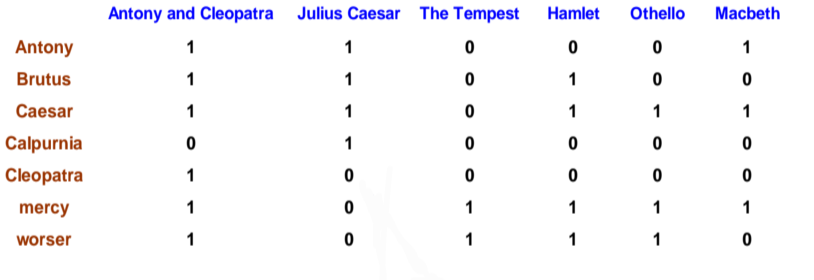
\includegraphics[scale=0.6]{assets/booleanmatrix.png}
	\end{center}

	\subsection{Vettori di Incidenza}
	Un'altra rappresentazione comune nel modello booleano è quella dei \textbf{vettori di incidenza}. In questa rappresentazione, un termine viene rappresentato da un'array di valori binari in cui ogni dimensione rappresenta un documento. Un valore di 1 indica la presenza del termine nel documento, mentre un valore di 0 indica l'assenza. 

	\paragraph{Esempio}
	Query: Brutus AND Caesar AND NOT Calpurnia
	\vspace{\baselineskip}\\
	\textbf{Brutus}: [1, 1, 0, 1, 0, 0]\\
	\textbf{Caesar}: [1, 1, 0, 1, 1, 1]\\
	\textbf{Calpurnia}: $\thicksim$ [0, 1, 0, 0, 0, 0] = [1, 0, 1, 1, 1, 1]
	\vspace{\baselineskip}\\
	\textbf{Risultato}: Bitwise AND tra Brutus e Caesar, e NOT Calpurnia = 110100 AND 110111 AND 101111 = 100100
	\vspace{\baselineskip}\\
	Quindi, i documenti 1 e 4 sono rilevanti rispetto alla query.

	\subsection{Indice Invertito}
	Un'implementazione pratica del modello booleano utilizza un \textbf{indice invertito} per associare ciascun termine ai documenti in cui appare. Questo indice consente di recuperare rapidamente i documenti rilevanti per una query, riducendo il tempo necessario per identificare i risultati. L'indice invertito è una struttura dati chiave-valore in cui le chiavi sono i termini e i valori sono degli identificatori \textit{docID} dei documenti in cui il termine appare. Per realizzare l'indice invertito, non possiamo utilizzare array a dimensipne fissa, ma strutture dati dinamiche come linked lists o altre strutture che permettono di aggiungere o rimuovere elementi in modo efficiente. L'insieme dei docId è detto \textbf{posting list}. Questo metodo non tiene conto del numero di occorrenze di un termine all'interno di un documento.

	\paragraph{Esempio}
	\begin{center}
		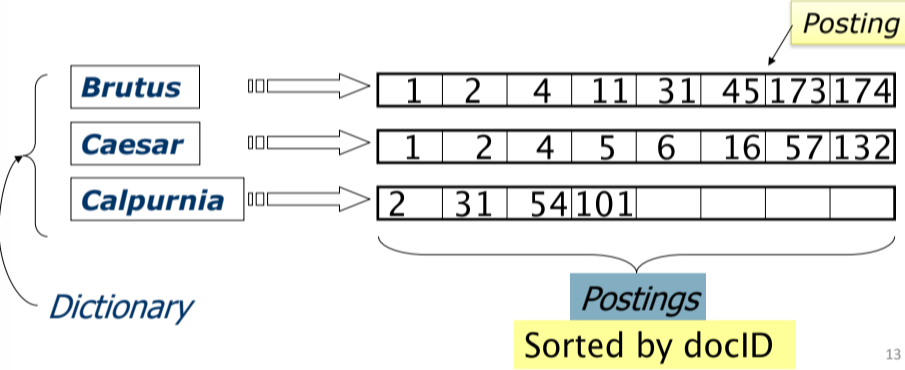
\includegraphics[scale=0.5]{assets/invertedindex.png}
	\end{center}

	Per costruire l'indice invertito, si parte da una collezione di documenti e si eseguono i seguenti passaggi:
	\begin{center}
		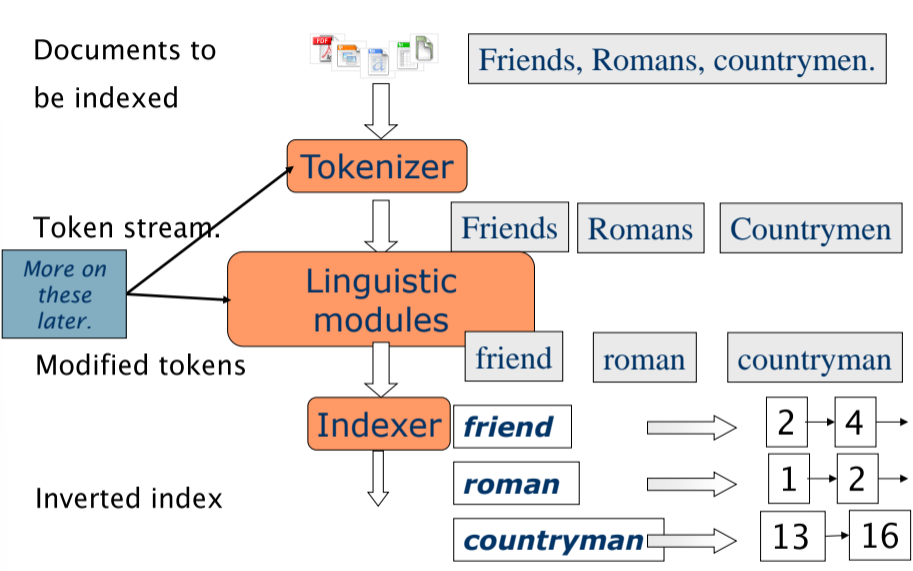
\includegraphics[scale=0.4]{assets/invindexconstr.png}
	\end{center}
	\begin{enumerate}
		\item Tokenizzazione: I documenti vengono suddivisi in token o termini.
		\item Modulazione linguistica: Rimozione delle stopwords, stemming e rimozione delle maiuscole.
		\item Costruzione dell'indice:
		\begin{itemize}
			\item Per ogni termine, si crea una posting list contenente gli identificatori dei documenti in cui il termine appare.
			\begin{center}
				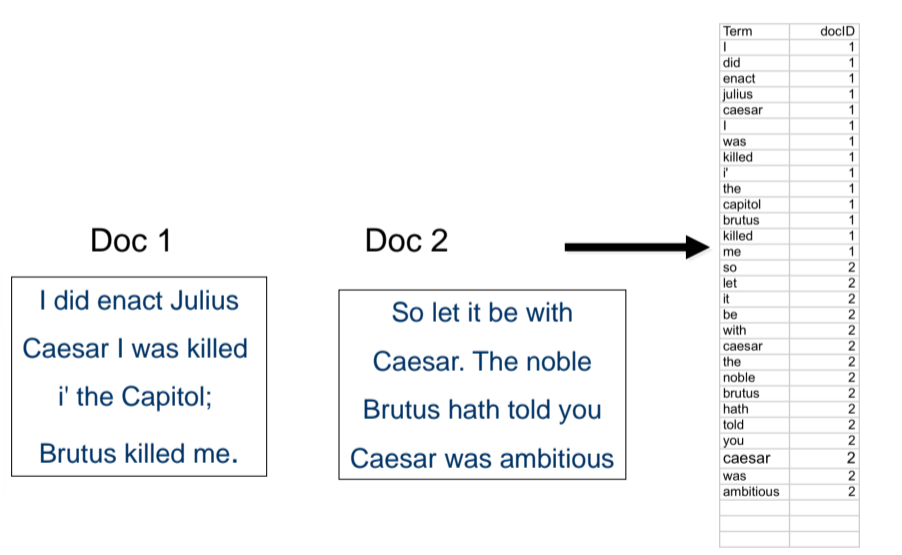
\includegraphics[scale=0.4]{assets/invindexposting.png}
			\end{center}
			\item Si ordinano i termini in ordine lessicografico e poi per docID.
			\begin{center}
				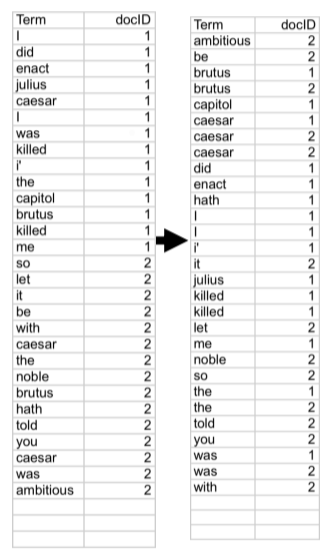
\includegraphics[scale=0.4]{assets/invindexsorted.png}
			\end{center}
			\item Vengono unite le entry dei termini duplicati tenendo conto del numero di documenti nei quali il termine appare e viene creata la posting list finale con i docID dei documenti in cui il termine appare. Il numero di documenti è una informazione ridondande ma utile per ottimizzare le operazioni di ricerca.
			\begin{center}
				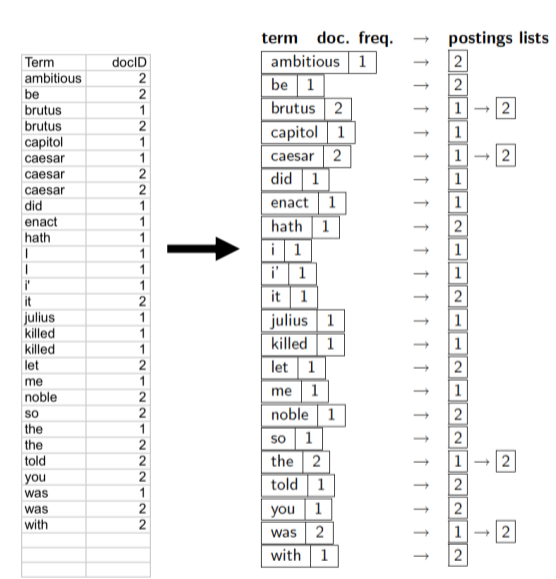
\includegraphics[scale=0.4]{assets/invindexfinal.png}
			\end{center}
		\end{itemize}
	\end{enumerate}

	\paragraph{Esempio}
	Consideriamo la query: \texttt{Brutus AND Caesar}. Per trovare i documenti rilevanti, localizziamo il termine "Brutus" nel dizionario e recuperiamo la posting list associata. Facciamo lo stesso per il termine "Caesar". Infine, eseguiamo un'operazione di intersezione tra le due posting list per trovare i documenti che contengono entrambi i termini. Le postings list sono ordinate per docID, quindi l'intersezione è un'operazione efficiente.
	\begin{center}
		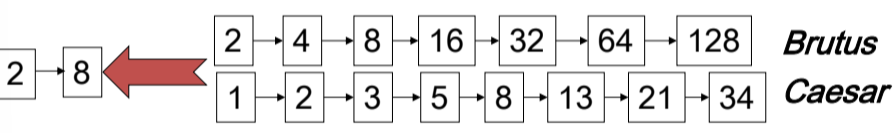
\includegraphics[scale=0.4]{assets/invindexexample.png}
	\end{center}

	\subsubsection{Algorimo di intersezione di due posting list}
	\begin{lstlisting}
		INTERSECT(P1, P2)
			answer = []
			while P1 not NIL and P2 not NIL
			do
				if docID(P1) = docID(P2)
				then
					ADD(answer, docID(P1))
					P1 = next(P1)
					P2 = next(P2)
				else if docID(P1) < docID(P2)
				then
					P1 = next(P1)
				else
					P2 = next(P2)
				end if
			end while
			return answer
	\end{lstlisting}

	\subsection{Problemi del Modello Booleano}
	Il Modello booleano è limitato dal fatto che l'operazione AND richiede che tutti i termini della query siano presenti nel documento per essere considerato rilevante. Questo può portare a risultati troppo restrittivi, in quanto i documenti che contengono solo alcuni dei termini della query non saranno considerati rilevanti. Allo stesso modo, l'operazione OR può portare a risultati troppo ampi, in quanto i documenti che contengono solo uno dei termini della query saranno considerati rilevanti. Inoltre, il modello deve andare a tradurre la query dell'utente in una serie di operatori logici, il che può essere complicato e non intuitivo per l'utente medio. Infine il modello non tiene conto della frequenza dei termini nei documenti, che potrebbe essere un indicatore di rilevanza. Di conseguenza, tutti i documenti matchati da una query hanno logicamente lo stesso livello di rilevanza. A questo si aggiunge l'impossibilità da parte dell'utente di esprimere un grado di rilevanza per i documenti recuperati.

	\section{Step di Pre-Processing}
	Il parsing dei documenti è il processo mediante il quale i contenuti di un documento vengono interpretati e strutturati per essere utilizzati da software o motori di ricerca. Può essere suddiviso in diverse fasi, ognuna delle quali svolge un compito specifico per interpretare e strutturare i contenuti del documento. Alcuni dei passaggi comuni del parsing dei documenti includono:
	\begin{itemize}		
		\item \textbf{Identificazione di formato, lingua e encoding}: 
		\begin{itemize}
			\item Una delle prime fasi del parsing consiste nel riconoscere il formato del documento (PDF, Word, Excel, HTML, ecc.), la lingua in cui è scritto e il set di caratteri utilizzato.
			\item Sebbene questo possa essere visto come un problema di classificazione, spesso la soluzione avviene tramite \textit{approcci euristici}, basati su regole semplici. Ad esempio: se un documento contiene molte occorrenze della parola "the", potrebbe essere classificato come documento in inglese.
		\end{itemize}
		\item \textbf{Complicazioni nella gestione di formati e lingue}:
		\begin{itemize}
			\item I documenti possono contenere formati e lingue multiple. Un esempio comune è un'email in francese con un allegato PDF in tedesco.
			\item Definire cosa costituisce una "unità di documento" non è sempre semplice: può essere un singolo file, un'email con più allegati o un insieme di file correlati (ad esempio, una presentazione PowerPoint con file associati o pagine HTML collegate).
		\end{itemize}
	\end{itemize}
	
	\subsection{Tokenizzazione}
	La tokenizzazione è il processo di suddivisione di un testo in unità più piccole, chiamate token che tipicamente corrispondono a parole o simboli. Questo passaggio è essenziale per l'analisi del testo, poiché consente di trattare le parole come unità atomiche e di eseguire operazioni su di esse. 

	\paragraph{Esempio}
	\begin{center}
		\textit{Testo originale: "Friends, Romans and Countrymen"}
		\textit{Token: ["Friends", "Romans", "Countrymen"]}
	\end{center}

	Durante la tokenizzazione, possono sorgere alcune sfide, come:
	\begin{itemize}
		\item \textbf{la gestione dei termini composti}: ad esempio, nella frase "Finland's capital", la prima parola può essere vista come "Finland", "Finlands" o "Finland's". Oppure,"Hewlett-Packard" può essere considerato come un singolo termine o come due termini separati.
		\item \textbf{la gestione dei numeri}: i numeri possono presentare diverse forme e formati, come "123", "1.23", "1,000", "1st", "2nd", ecc.  Spesso i numeri presentano spazi o virgole che possono complicare la tokenizzazione.
		\item \textbf{la gestione delle date}: le date possono essere scritte in diversi formati, come "3/20/91", "Mar. 12, 1991" o "20/3/91".
		\item \textbf{la gestione delle lingue}: ad esempio, nella parola francese "l'ensemble", si potrebbe vedere l'articolo come "l", "l'" o "le". Oppure, nel caso della lingua tedesca i sostantivi composti non sono separati da spazi, come ad esempio "Lebensversicherungsgesellschaftsangestellter", che significa "impiegato di una compagnia di assicurazioni sulla vita". O ancora, in cinese e in giapponese non esistono spazi tra le parole. In arabo la scrittura è da destra a sinistra e le vocali non sono scritte.
	\end{itemize}

	\subsection{Rimozione delle Stopwords}
	Le \textbf{stopwords} sono parole comuni che vengono spesso rimosse durante il pre-processing del testo poiché non aggiungono significato o rilevanza al contenuto. Queste parole includono articoli, preposizioni, congiunzioni e altre parole di uso comune che non portano informazioni specifiche. La rimozione delle stopwords aiuta a ridurre il rumore nei dati e a concentrarsi sui termini più significativi. In alcuni casi, tuttavia, le stopwords possono essere rilevanti per il contesto e non dovrebbero essere rimosse. Ad esempio, nel caso di titoli di libri o canzoni, o nelle locuzioni e titoli nobiliari.

	\subsection{Normalizzazione}
	La normalizzazione è il processo di trasformazione del testo in una forma standardizzata o normalizzata. Questo passaggio è utile per ridurre la complessità e la variabilità del testo, consentendo di confrontare e analizzare i dati in modo più efficiente. Ad esempio, il termine "U.S.A" può essere normalizzato in "USA", poichè vogliamo considerare entrambi i termini come equivalenti. Oppure il termine "anti-discriminatorio" può essere normalizzato in "antidiscriminatorio" per evitare ambiguità. Nel campo delle lingue, gli accenti e le dieresi vengono spesso rimossi per semplificare la tokenizzazione e la ricerca.

	\subsection{Case Folding}
	La case folding è il processo di conversione di tutte le lettere di un testo in minuscolo, ad ecezione dei casi in cui la distinzione tra maiuscole e minuscole è rilevante. Questo passaggio è utile per uniformare il testo e semplificare le operazioni di confronto e ricerca. Ad esempio, la parola "Apple" e "apple" dovrebbero essere considerate equivalenti durante la tokenizzazione e la ricerca.

	\subsection{Normalizzazione ai termini}
	Un'alternativa per equivalere la classificazione dei termini è la normalizzazione ai termini. Questo processo consiste nell'includere nel dizionario molte varianti di un termine per poi fare un'espansione asimmetrica al momento della query. Ad esempio, il termine "window" potrebbe essere espanso in "window", "windows", "windowing", "windowed", ecc. E' potenzialmente più costoso in termini di spazio ma permette di evitare di perdere informazioni.

	\subsection{Thesauri and Soundex}
	Un altro punto focale è la gestione dei sinonimi e degli omonimi. I sinonimi sono parole che hanno lo stesso significato, mentre gli omonimi sono parole che si scrivono allo stesso modo ma hanno significati diversi. Per gestire questi casi, si possono utilizzare thesauri, dizionari di sinonimi, e Soundex, un algoritmo fonetico per la ricerca di parole simili foneticamente. Questo può essere effettuabile tramite costrutti di equivalenza tra termini, come ad esempio "car" e "automobile" che vengono memorizzati come "car - automobile" oppure possiamo espandere la query che contiene "automobile" cercando anche "car".
	\vspace{\baselineskip}\\
	Nel caso degli errori di spelling, un approccio sono i soundex che creano classi di equivalenza per parole che si basano sulla stessa euristica fonetica. Ad esempio, "Smith" e "Smyth" avrebbero lo stesso codice soundex. Questo permette di trovare parole simili anche se scritte in modo diverso.

	\subsection{Lemmatizzazione}
	La lemmatizzazione è il processo di riduzione delle parole alla loro forma base, chiamata lemma. Questo passaggio è utile per ridurre i termini alla loro forma canonica e semplificare l'analisi del testo. Ad esempio, i termini "am", "are" o "is" possono essere ridotti alla forma base "be". 

	\subsection{Stemming}
	Lo stemming è il processo di riduzione delle parole alla loro radice o stem, rimuovendo eventuali suffissi o prefissi. Questo passaggio è utile per ridurre i termini alla loro forma base e semplificare l'analisi del testo. Ad esempio, i termini "automate", "automatic" o "automation" possono essere ridotti ad "automat".

	\subsubsection{Algoritmo di Porter}
	L'algoritmo di Porter è il più comune per quanto riguarda lo stemming della lingua inglese. Esso è un algoritmo basato su regole che riduce le parole inglesi alla loro forma base. L'algoritmo di Porter è diviso in diverse fasi sequenziali, ognuna delle quali applica regole specifiche per ridurre le parole alla loro forma base. 
	\paragraph{Esempio}
	\textit{Testo di Partenza}: Such an analysis can reveal features that are not easily visible from the variations in the individual genes and can lead to a picture of expression that is more biologically transparent and accessible to interpretation
	\vspace{\baselineskip}\\
	\textit{Porter Stemming}: such an analysi can reveal featur that ar not easili visibl from the variat in the individu gene and can lead to a pictur of express that is more biolog transpar and access to interpret

	\chapter{Scoring, Term Weighting e Modelli a Spazio Vettoriale}
	\section{Boolean Retrieval}
	Le query che abbiamo utilizzato finora sono di tipo booleano. In questo modello di ricerca, i documenti o corrispondono alla query o non lo fanno. Questo approccio è efficace per utenti esperti che possiedono una comprensione precisa sia delle loro esigenze che della collezione di documenti. È anche utile per applicazioni che devono gestire migliaia di risultati in maniera automatizzata.
	\vspace{\baselineskip}\\
	Tuttavia, questo modello non è adatto alla maggior parte degli utenti, in quanto molti non sono in grado di scrivere query booleane complesse o lo trovano un compito troppo gravoso. Inoltre, la maggior parte degli utenti non ha il desiderio o il tempo di analizzare migliaia di risultati, come accade spesso nelle ricerche sul web.

	\subsection{Problema del Modello Booleano: Sovrabbondanza o Carestia}
	Le query booleane tendono a generare o troppo pochi risultati (spesso zero) o troppi (migliaia). Ad esempio:

	\begin{itemize}
    	\item Query 1: \texttt{"standard user dlink 650"} genera 200.000 risultati.
    	\item Query 2: \texttt{"standard user dlink 650 no card found"} non produce alcun risultato.
	\end{itemize}

	È necessaria una notevole abilità per costruire una query che produca un numero gestibile di risultati. Le query con l'operatore \texttt{AND} tendono a restituire pochi risultati, mentre l'operatore \texttt{OR} ne genera troppi.

	\section{Ranked Retrieval Models}
	Diversamente dalle query booleane, i modelli di recupero basati su classifiche non cercano semplicemente di restituire un insieme di documenti che soddisfano una specifica query. Invece, ordinano i documenti in base alla loro rilevanza rispetto alla query. Le query in linguaggio naturale sono esempi tipici di questo approccio. Invece di usare una lingua formale fatta di operatori e espressioni, l'utente inserisce una o più parole in linguaggio naturale per esprimere la sua ricerca.
	\vspace{\baselineskip}\\
	In linea di principio, ci sono due scelte separate da considerare:
	\begin{itemize}
    	\item Il \textbf{linguaggio di query}, che può essere formale o in linguaggio naturale.
    	\item Il \textbf{modello di recupero}, che può essere booleano o basato su classifiche.
	\end{itemize}
	Nella pratica, i modelli di recupero basati su classifiche sono comunemente associati a query in linguaggio naturale.

	\section{Problema della Dimensione dei Set di Risultati}
	Una delle preoccupazioni più frequenti è la gestione di set di risultati di grandi dimensioni. Tuttavia, questo non è un vero problema quando si utilizzano sistemi di recupero che producono risultati ordinati. Infatti, la dimensione del set di risultati non rappresenta un ostacolo, poiché normalmente viene mostrata solo una selezione dei migliori risultati, in genere i primi $k$, dove $k$ è un numero intorno a 10.
	\vspace{\baselineskip}\\
	Questo approccio mira a evitare di sopraffare l'utente con troppi risultati. L'assunzione fondamentale dietro questa strategia è che l'algoritmo di ranking funzioni correttamente, cioè che i risultati mostrati in cima alla lista siano effettivamente i più rilevanti per la query. Ora, possiamo davvero affermare che non ci siano problemi con set di grandi dimensioni se l'algoritmo di ranking funziona bene? Ciò apre una riflessione più ampia sull'importanza di un buon ordinamento, poiché un algoritmo di ranking che fallisce nel distinguere la rilevanza tra i risultati potrebbe comunque causare problemi anche con un numero ridotto di risultati mostrati.

	\section{Scoring}
	Il ranking dei documenti è basato sulla capacità di attribuire a ciascun documento un punteggio, che rappresenta quanto quel documento sia rilevante rispetto alla query dell'utente. L'obiettivo di questo processo è quello di restituire i documenti in un ordine che riflette la loro utilità per l'utente. Per ottenere questo, dobbiamo ordinare i documenti in base alla loro rilevanza rispetto alla query. Questo si ottiene assegnando a ogni documento un punteggio, tipicamente compreso tra 0 e 1, che rappresenta la corrispondenza tra il documento e la query. Un punteggio più vicino a 1 indicherà una maggiore affinità tra il documento e la query, mentre un punteggio vicino a 0 indicherà che il documento è poco pertinente. Questo sistema permette al motore di ricerca di ordinare i documenti in modo che quelli più pertinenti compaiano nelle prime posizioni, migliorando così l'efficienza del recupero e l'esperienza dell'utente.
	\vspace{\baselineskip}\\
	Per poter ordinare correttamente i documenti rispetto a una query, è necessario disporre di un meccanismo che assegni un punteggio a ogni coppia documento-query. Per semplificare, possiamo iniziare a considerare il caso di una query composta da un solo termine. Nel caso in cui il termine della query non sia presente nel documento, il punteggio assegnato sarà 0, poiché non esiste alcuna corrispondenza diretta tra query e documento. Tuttavia, possiamo chiederci: è possibile fare di meglio? Forse potremmo considerare altre informazioni, come la semantica del termine o sinonimi, per migliorare il punteggio anche quando il termine esatto non è presente. Inoltre, se il termine della query compare nel documento, il punteggio dovrebbe aumentare proporzionalmente alla frequenza con cui il termine appare. Questo riflette l'idea che più un documento contiene il termine della query, più è probabile che sia rilevante per l'utente. Esistono comunque diverse alternative per il calcolo del punteggio, che prenderemo in considerazione.

	\subsection{Coefficiente di Jaccard}
	Per assegnare un punteggio di rilevanza tra la query dell'utente e i documenti, possiamo fare uso di diverse metriche. Una delle più comuni è il \textbf{coefficiente di Jaccard}, che misura l'overlap tra due insiemi. Nel nostro caso, possiamo rappresentare la query e il documento come insiemi di termini e calcolare il loro grado di sovrapposizione.\\
	Il \textbf{coefficiente di Jaccard} viene calcolato come segue:
	\[
	\text{jaccard}(A, B) = \frac{|A \cap B|}{|A \cup B|}
	\]
	dove \( A \) rappresenta l'insieme di termini della query e \( B \) l'insieme di termini di un documento. Il valore di questo coefficiente varia tra 0 e 1. Se il coefficiente è 1, significa che i termini della query e del documento coincidono perfettamente. Se il coefficiente è 0, non ci sono termini in comune tra la query e il documento.
	\vspace{\baselineskip}\\
	Per esempio:
	\begin{itemize}
		\item Data una query "ides of march" e due documenti con i termini "caesar died in march" e "the long march", otteniamo i seguenti punteggi Jaccard:
		\begin{itemize}
			\item Documento 1: \( \frac{1}{6} \)
			\item Documento 2: \( \frac{1}{5} \)
		\end{itemize}
	\end{itemize}
	In questo caso, il primo documento risulta meno rilevante del secondo rispetto alla query "ides of march", in quanto la sovrapposizione dei termini è minore.

	Tuttavia, il coefficiente di Jaccard presenta alcune limitazioni. Non tiene conto della \textbf{frequenza dei termini} all'interno del documento, ignorando quindi quante volte un termine appare. Inoltre, non differenzia tra termini comuni e rari, trascurando il fatto che termini meno frequenti sono spesso più informativi. Infine, il metodo non normalizza in base alla lunghezza dei documenti, il che può influire sulla qualità del ranking.

	Questo approccio introduce una prima misura di affinità tra query e documenti, utile per ordinare i risultati. Tuttavia, come indicato, è necessario valutare metodi più sofisticati per migliorare il ranking e affinare l'esperienza dell'utente, considerando aspetti come la frequenza dei termini e l’importanza delle parole.

	\subsection{Matrici di Incidenza Binarie VS Matrici di Frequenza}
	Un modo comune per rappresentare l'associazione tra termini e documenti è attraverso una \textbf{matrice di incidenza binaria}. In questa matrice, le righe rappresentano i termini presenti nel vocabolario e le colonne rappresentano i documenti. L'elemento \( a_{ij} \) della matrice vale 1 se il termine \( i \) è presente nel documento \( j \), e 0 altrimenti. Questo tipo di rappresentazione è utile per determinare la presenza o l'assenza di termini in ciascun documento.
	Ad esempio, una matrice di incidenza binaria per tre termini (\texttt{t1, t2, t3}) e tre documenti (\texttt{d1, d2, d3}) può essere rappresentata come segue:
	\[
	\begin{array}{c|ccc}
	& d1 & d2 & d3 \\
	\hline
	t1 & 1 & 0 & 1 \\
	t2 & 1 & 1 & 0 \\
	t3 & 0 & 1 & 1 \\
	\end{array}
	\]
	In questa matrice, il termine \( t1 \) è presente in \( d1 \) e \( d3 \), mentre il termine \( t2 \) è presente in \( d1 \) e \( d2 \), e così via.
	Tuttavia, la matrice di incidenza binaria presenta una limitazione importante: non tiene conto della \textbf{frequenza} dei termini. Essa considera solo se un termine è presente o assente, ma non registra il numero di occorrenze del termine in ciascun documento. Questo è problematico in quanto, generalmente, termini con frequenze più alte all'interno di un documento tendono ad essere più rilevanti per quel documento.
	Per superare questa limitazione, si utilizza una \textbf{matrice di conteggio termine-documento}. In questa rappresentazione, l'elemento \( c_{ij} \) della matrice rappresenta il numero di volte in cui il termine \( i \) appare nel documento \( j \). Questa matrice di conteggio permette di mantenere l'informazione sulla frequenza dei termini, offrendo una rappresentazione più accurata della rilevanza di ciascun termine rispetto a ogni documento.
	Ad esempio, una matrice di conteggio per gli stessi termini e documenti potrebbe apparire come:
	\[
	\begin{array}{c|ccc}
	& d1 & d2 & d3 \\
	\hline
	t1 & 2 & 0 & 3 \\
	t2 & 1 & 4 & 0 \\
	t3 & 0 & 1 & 2 \\
	\end{array}
	\]
	In questa matrice, il termine \( t1 \) appare due volte in \( d1 \) e tre volte in \( d3 \), mentre il termine \( t2 \) appare una volta in \( d1 \) e quattro volte in \( d2 \), e così via. Rispetto alla matrice binaria, questo approccio consente di costruire modelli di scoring più sofisticati che possono riflettere meglio la rilevanza dei documenti in relazione alla query dell'utente.
	Va notato, tuttavia, che i vettori di rappresentazione della matrice di conteggio non tengono conto dell'ordine delle parole nei documenti. Questo modello di rappresentazione, chiamato \textbf{bag of words}, tratta ogni documento come una semplice collezione di parole, ignorando la sequenza con cui queste compaiono. Di conseguenza, due documenti con gli stessi termini, ma in un ordine diverso, avranno lo stesso vettore di rappresentazione. Questo approccio è efficace per molti algoritmi di recupero dell'informazione e classificazione, ma perde informazioni semantiche relative alla struttura e al contesto della frase.

	\subsection{Term Frequency (TF)}
	Un modo comune per calcolare il punteggio di rilevanza di un documento rispetto a una query è utilizzare la \textbf{term frequency} (TF). La term frequency $tf_{t,d}$ è il numero di volte che un termine t appare in un documento d. D'altro canto la rilevanza di un documento rispetto alla query non aumenta proporzionalmente alla tf. Infatti, se un termine appare molte volte in un documento, non significa necessariamente che il documento sia più rilevante per la query. Per questo motivo, è necessario non considerare il dato grezzo della term frequency, ma normalizzarlo in qualche modo. 

	\subsection{Log-Frequency Weighting}
	Un modo per normalizzare la term frequency è utilizzare il \textbf{log-frequency weighting}. Questo metodo consiste nel calcolare il logaritmo della term frequency per ridurre l'impatto delle frequenze più alte. In questo modo, la term frequency viene trasformata in una scala logaritmica, che riduce la differenza tra i valori più alti e quelli più bassi. Nello specifico, la log-frequency weighting è definita come:
	\[
	w_{t,d} = \begin{cases}
		1 + \log_{10}(tf_{t,d}) & \text{se } tf_{t,d} > 0 \\
		0 & \text{altrimenti}
	\end{cases}
	\]
	Lo score per un documento d rispetto a una query q è quindi calcolato come la somma dei pesi dei termini presenti nella query:
	\[
	\text{score}(q,d) = \sum_{t \in q \cap d} w_{t,d}
	\]
	Lo score è 0 se nessun termine della query è presente nel documento.
	\vspace{\baselineskip}\\
	La formula della log-frequency weighting definisce lo \textbf{sublinear tf-scaling} che tendenzialmente dovrebbe essere preferibile rispetto all'approccio normale della term frequency.

	\subsection{Document Frequency (DF)}
	Un'altra misura importante per valutare la rilevanza di un termine rispetto a una query è la \textbf{document frequency} (DF). La document frequency $df_t$ è il numero di documenti d in cui il termine t appare. Questa misura è utile per valutare l'importanza di un termine all'interno di una collezione di documenti. Ad esempio, un termine che appare in molti documenti potrebbe non essere molto discriminante, mentre un termine che appare in pochi documenti potrebbe essere più informativo. Nello specifico, definiamo la \textbf{inverse document frequency} (IDF) come il logaritmo del rapporto tra il numero totale di documenti e il document frequency di un termine:
	\[
	\text{idf}_t = \log\left(\frac{N}{df_t}\right)
	\]
	dove N è il numero totale di documenti nella collezione. L'idf è una misura di quanto un termine sia comune o raro all'interno della collezione. I termini che appaiono in molti documenti avranno un valore di idf più basso, mentre i termini che appaiono in pochi documenti avranno un valore di idf più alto. Questo è utile perché i termini rari sono spesso più informativi rispetto ai termini comuni. L'idf è spesso utilizzato in combinazione con la term frequency per calcolare il peso di un termine rispetto a un documento.
	\vspace{\baselineskip}\\
	Nonostante ciò, l'idf non ha effetto sul ranking dei documenti per query che contengono un solo termine.

	\subsection{Collection Frequency (CF)}
	A differenza della DF, la \textbf{Collection Frequency} (CF) è il numero totale di occorrenze di un termine in tutta la collezione di documenti. Questa misura è utile per valutare la frequenza assoluta di un termine all'interno della collezione. 

	\subsection{Term Frequency-Inverse Document Frequency (TF-IDF)}
	Una delle misure più comuni per calcolare il peso di un termine rispetto a un documento è il \textbf{Term Frequency-Inverse Document Frequency} (TF-IDF). Questo metodo combina la term frequency e l'inverse document frequency per calcolare il peso di un termine rispetto a un documento. Il peso di un termine t rispetto a un documento d è calcolato come il prodotto della term frequency e dell'inverse document frequency:
	\[
	\text{w}_{t,d} = \text{tf}_{t,d} \times \text{idf}_t = (1 + \log_{10}(\text{tf}_{t,d})) \times \log_{10}\left(\frac{N}{\text{df}_t}\right)
	\]
	Questo metodo assegna un peso maggiore ai termini che compaiono frequentemente in un documento ma raramente in altri documenti. In questo modo, i termini che sono più informativi e discriminanti vengono premiati con un peso più alto. Il punteggio di un documento d rispetto a una query q è calcolato come la somma dei pesi dei termini presenti nella query:
	\[
	\text{score}(q,d) = \sum_{t \in q \cap d} (tf_{t,d} \times \text{idf}_t)
	\]
	A questo punto possiamo introdurre una nuova matrice di incidenza, la \textbf{matrice TF-IDF}, che rappresenta i pesi dei termini rispetto ai documenti.
	
	\section{Modelli a Spazio Vettoriale}
	\subsection{Documents as Vectors}
	Un modo comune per rappresentare i documenti è attraverso vettori. In questo modello, ogni documento è rappresentato come un vettore in uno spazio multidimensionale, dove ogni dimensione corrisponde a un termine. I termini sono le assi dello spazio, mentre i documenti sono i punti all'interno di questo spazio. La posizione di un documento nello spazio è determinata dai pesi dei termini che lo compongono. Questo modello è noto come \textbf{modello a spazio vettoriale}.

	\subsection{Query as Vectors}
	Analogamente, le query possono essere rappresentate come vettori nello stesso spazio multidimensionale. In questo modo, possiamo confrontare i vettori dei documenti con il vettore della query per determinare la loro rilevanza in base alla loro prossimità nello spazio vettoriale. 

	\subsection{Formalizzare la Prossimità nello Spazio Vettoriale}
	Per calcolare la prossimità tra i vettori dei documenti e il vettore della query, possiamo utilizzare diverse metriche di similarità. Inizialmente si pensò di utilizzare la distanza fra due punti, ma l'incognita era quale distanza utilizzare. Nel caso della distanza euclidea, si ebbe il problema che i documenti più lunghi avrebbero avuto una distanza maggiore rispetto ai documenti più corti. A questo punto si decise di utilizzare l'angolo tra i vettori, anzichè la distanza. Se la query e il documento sono simili, l'angolo tra i due vettori sarà piccolo, mentre se sono dissimili, l'angolo sarà grande. Nel caso della $tf_{t,d}$ se l'angolo è 0, allora c'è massima similarità. Dagli angoli si passò a utilizzare il coseno dell'angolo per un semplice motivo: il coseno è una funzione monotona decrescente dell'angolo, quindi se due vettori sono simili, il coseno sarà vicino a 1, mentre se sono dissimili, il coseno sarà vicino a 0.
	
	\subsection{Normalizzazione della Lunghezza}
	Un problema che si presenta è che i documenti più lunghi avranno vettori più lunghi rispetto ai documenti più corti. Questo potrebbe portare a una distorsione della similarità tra i documenti. Per risolvere questo problema, si normalizzano i vettori dei documenti dividendo ogni componente per la lunghezza del vettore. In questo modo, tutti i vettori avranno la stessa lunghezza, indipendentemente dalla lunghezza del documento. Questo processo è noto come \textbf{normalizzazione della lunghezza}. Nel nostro caso, utilizzeremo la normalizzazione L2 che è definita come:
	\[
	\| \overrightarrow{x}  \|_{2} = \sqrt{\sum_{i} x_{i}^{2}} 
	\]

	\subsection{Similarità del Coseno}
	Come detto in precedenza, la similarità del coseno è una misura di similarità tra due vettori nello spazio vettoriale. Questa misura è calcolata come il coseno dell'angolo tra il vettore documento e il vettore query. La similarità del coseno è definita come:
	\[
	\text{cos}(\overrightarrow{q}, \overrightarrow{d}) = \frac{\overrightarrow{q} \cdot \overrightarrow{d}}{\| \overrightarrow{q} \| \times \| \overrightarrow{d} \|} = \frac{\sum_{i} q_{i} \times d_{i}}{\sqrt{\sum_{i=1}^{|V|} q_{i}^{2}} \times \sqrt{\sum_{i}^{|V|} d_{i}^{2}}}
	\]
	dove $q_i$ è il $tf-idf$ del termine i nella query, $d_i$ è il $tf-idf$ del termine i nel documento e $V$ è il vocabolario. $cos(\overrightarrow{q}, \overrightarrow{d})$ è la similarità tra $\overrightarrow{q}$ e $\overrightarrow{d}$ o, similarmente, il coseno dell'angolo tra i due vettori.
	\vspace{\baselineskip}\\
	La similarità del coseno può essere utilizzata anche con vettori di lunghezza normalizzata, in quanto la similarità del coseno è indipendente dalla lunghezza dei vettori. Questo significa che possiamo confrontare i documenti in base alla loro rilevanza rispetto alla query, indipendentemente dalla loro lunghezza.
	Nel caso di vettori con lunghezza normalizzata, la similarità del coseno è semplicemente il prodotto scalare tra i due vettori, ovvero:
	\[
	\text{cos}(\overrightarrow{q}, \overrightarrow{d}) = \overrightarrow{q} \cdot \overrightarrow{d} = \sum_{i=1}^{|V|} q_{i} \times d_{i}
	\]
	\begin{algorithm}[H]
		\caption{CosineScore($q$)}
		\begin{algorithmic}
			\State float Scores[$N$] = 0
			\State float Length[$N$]
			\ForAll{pair(d, $tf_{t,d}$) in postings list}
				\State Scores[d] += $w_{t,d} \times w_{t,q}$
			\EndFor
			\State read Length
			\ForAll{d}
				\State Scores[d] = Scores[d] / Length[d]
			\EndFor
			\State \Return Top K components of Scores
		\end{algorithmic}
	\end{algorithm}
	
	\paragraph{Esempio}
	Quanto sono simili le poesie "Sas: Sense and Sensibility", "PaP: Pride and Prejudice" e "WH: Wuthering Heights"?

	\textbf{Term Frequencies counts}:
	\begin{table}[H]
		\centering
		\begin{tabular}{|c|c|c|c|}
			\hline
			 term & Sas & PaP & WH \\
			\hline
			 affection & 115 & 58 & 20 \\
			 jealous & 10 & 7 & 11 \\
			 gossip & 2 & 0 & 6 \\
			 wuthering & 0 & 0 & 38 \\
			\hline
		\end{tabular} 
	\end{table}
	\textbf{Log Frequencies weighting}:
	\begin{table}[H]
		\centering
		\begin{tabular}{|c|c|c|c|}
			\hline
			 term & Sas & PaP & WH \\
			\hline
			 affection & 3.06 & 2.76 & 2.30 \\
			 jealous & 2.00 & 1.85 & 2.04 \\
			 gossip & 1.30 & 0 & 1.78 \\
			 wuthering & 0 & 0 & 2.58 \\
			\hline
		\end{tabular} 
	\end{table}
	\textbf{After length normalization}:
	\begin{table}[H]
		\centering
		\begin{tabular}{|c|c|c|c|}
			\hline
			 term & Sas & PaP & WH \\
			\hline
			 affection & 0.789 & 0.832 & 0.524 \\
			 jealous & 0.515 & 0.555 & 0.465 \\
			 gossip & 0.335 & 0 & 0.405 \\
			 wuthering & 0 & 0 & 0.588 \\
			\hline
		\end{tabular} 
	\end{table}
	\[
		\text{cos}(Sas, PaP) \approx 0.789 \times 0.832 + 0.515 \times 0.555 + 0.335 \times 0 + 0 \times 0 \approx 0.94 
	\]
	\[
		\text{cos}(Sas, WH) \approx 0.79
	\]
	\[
		\text{cos}(PaP, WH) \approx 0.69
	\]
	Abbiamo che $cos(Sas, PaP) > cos(Sas, WH) > cos(PaP, WH)$, quindi la poesia "Sas: Sense and Sensibility" è più simile a "PaP: Pride and Prejudice" rispetto a "WH: Wuthering Heights". Questo perchè "Sas" e "PaP" condividono più termini rispetto a "Sas" e "WH".

	\subsection{Varianti del tf-idf}
	\begin{table}[H]
		\centering
		\renewcommand{\arraystretch}{1.5}
		\begin{tabular}{|c|c|c|c|}
		\hline
		\textbf{Term frequency} & \textbf{Document frequency} & \textbf{Normalization} \\
		\hline
		{n (natural)} & {n (no)} & {n (none)} \\
		$tf_{t,d}$ & $1$ & $1$ \\
		\hline
		{l (logarithm)} & {t (idf)} & {c (cosine)} \\
		$1 + \log(tf_{t,d})$ & $\log \frac{N}{df_t}$ & $\frac{1}{\sqrt{w_1^2 + w_2^2 + \cdots + w_M^2}}$ \\
		\hline
		a (augmented) & p (prob idf) & u (pivoted unique) \\
		$0.5 + \frac{0.5 \cdot tf_{t,d}}{\max(tf_{t,d})}$ & $\max \{0, \log \frac{N - df_t}{df_t} \}$ & $\frac{1}{u}$ \\
		\hline
		b (boolean) & & b (byte size) \\
		$\begin{cases} 1 & \text{if } tf_{t,d} > 0 \\ 0 & \text{otherwise} \end{cases}$ & & $\frac{1}{\text{CharLength}^\alpha}, \alpha < 1$ \\
		\hline
		L (log ave) & & \\
		$\frac{1 + \log(tf_{t,d})}{1 + \log(\text{ave}_{t \in d}(tf_{t,d}))}$ & & \\
		\hline
		\end{tabular}
	\end{table}

	\subsection{Scelte del metodo di Weighting}
	Molti motori di ricerca permettono di utilizzare metodi di weighting differenti applicabili sulle query e sui documenti. In questo caso viene utilizzata una notazione che combina il weighting dei documenti con il weighting delle query separate da un punto (ddd.qqq) ove ddd e qqq corrispondono agli acronimi della tabella precedente.
	
	\chapter{Integrazione di conoscenza Lessicale}
	\section{WordNet}
	\textbf{WordNet} è un ontologia linguistica top-level, un database lessicale della lingua inglese che raggruppa le parole in gruppi di sinonimi, fornendo definizioni e relazioni semantiche tra i termini. WordNet è organizzato in un grafo aciclico diretto, in cui i nodi rappresentano i termini e gli archi rappresentano le relazioni tra i termini. Molti sistemi di IR e Text Categorization utilizzano la conoscenza linguistica di WordNet per aggiungere semantica al processo di ritrovamento o di categorizzazione. Gli ideatori di WordNet si sono ispirati alla suddivisione della memoria lessicale umana, applicandola in modo analogo alla sua conoscenza lessicale. La suddivisione è composta da sostantivi, verbi, aggettivi e avverbi.

	\subsection{Concetto di Parola}
	La parola è una associazione fra una word form e una word meaning.
	\vspace{\baselineskip}\\
	La \textbf{word form} è l'espressione fisica della parola, ovvero l'insieme di lettere che la costituisce. La \textbf{word meaning} è il concetto lessicale che la word form vuole esprimere, quindi il suo significato sottinteso. I sinonimi hanno stessa word meaning e word form diversa, mentre i polisemi hanno stessa word form e word meaning diversa.

	\subsection{Matrice Lessicale}
	WordNet è strutturato su una matrice lessicale che realizza un mapping fra word form e word meaning.
	\begin{table}[h!]
		\centering
		\renewcommand{\arraystretch}{1.5}
		\begin{tabular}{|c|c|c|c|c|c|}
			\hline
			\multicolumn{1}{|c|}{\textbf{Word Meanings}} & \multicolumn{5}{c|}{\textbf{Word Forms}} \\ \hline
			& $F_1$ & $F_2$ & $F_3$ & $\cdots$ & $F_n$ \\ \hline
			$M_1$ & $V(1,1)$ & $V(2,1)$ & & & \\ \hline
			$M_2$ & & $V(2,2)$ & $V(3,2)$ & & \\ \hline
			$M_3$ & & & & & \\ \hline
			$M_{\dots}$ & & & & & \\ \hline
			$M_m$ & & & & & $V(m,n)$ \\ \hline
		\end{tabular}
	\end{table}
	
	\subsection{Rappresentazione della conoscenza linguistica}
	Lo scopo principale di WordNet è quello di riuscire a trasferire ad un coomputer tutta la conoscenza linguistica, quindi le word form, le word meaning e il mapping fra le due categorie.
	\vspace{\baselineskip}\\
	La rappresentazioe delle word form in una forma comprensibile ad un calcolatore non ha suscitato molti problemi, in quanto si tratta di una sequenza di caratteri. La rappresentazione delle word meaning è stata più complessa, in quanto si tratta di concetti astratti e non fisici. Per questo motivo, si è deciso di rappresentare le word meaning come insieme di word form che possono essere usate per esprimerla, il \textbf{Synset (Synonymous Set)}. 
	\vspace{\baselineskip}\\
	Un Synset associato ad una word form consente all'utente di inferire la semnantica della word form in esame purchè si conosca la semantica di almeno una word form elencata nel synset. \\
	I synset sono legati da relazioni sui sostantivi:
	\begin{itemize}
		\item \textbf{Relazione Gerarchica (is-a)} che collega i synset in una gerarchia percorribile in entrambe le direzioni. Per questo si suddivide in:
		\begin{itemize}
			\item \textbf{Iperonimia}: relazione che va da un termine specifico ad uno più generico (mobile iperonimo di sedia quindi si va da sedia a mobile).
			\item \textbf{Iponimia}: relazione che va da un termine generico ad uno più specifico (pino iponimo di albero quindi si va da albero a pino).
		\end{itemize}
		\item \textbf{Relazione di Tutto-Parti} che collega i synset in una relazione di inclusione. Si suddivide in due tipi:
		\begin{itemize}
			\item \textbf{Meronimia}: relazione termine costituente che indica una parte, o un membro, e un termine che indica l'intero. X è meronimo di Y se X è parte di Y, o X è meronimo di Y se X è un membro di Y (dito è meronimo di mano).
			\item \textbf{Olonimia}: relazione tra un termine che indica l'intero (l'olonimo) e un termine che ne rappresenta una parte, o un membro. X è un olonimo di Y se Y è parte di X, o X è un olonimo di Y se Y è membro di X (albero è un olonimo di 'corteccia', o 'tronco')
		\end{itemize}
	\end{itemize}
	Tornando alla matrice lessicale, il synset non è altro che un record di associazione tra word form e word meaning. La matrice lessicale è una matrice sparsa, in quanto non tutte le word form sono associate a tutte le word meaning.
	\begin{center}
		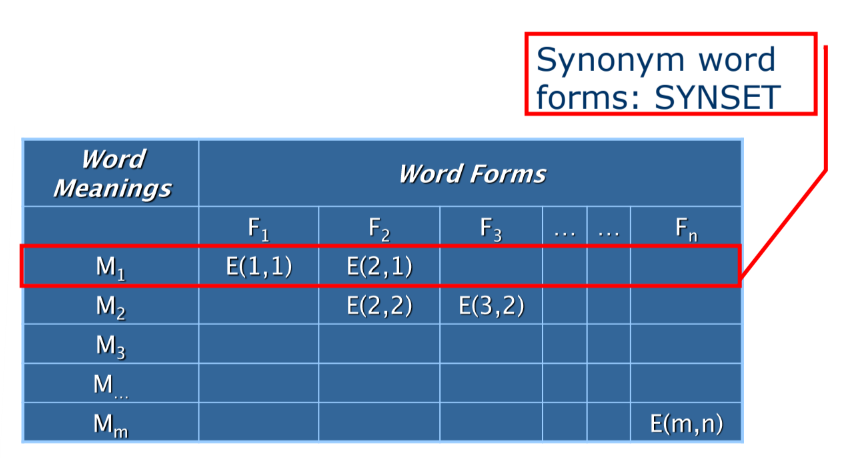
\includegraphics[scale=0.5]{assets/lex-mat-syn.png}
	\end{center}
	\begin{center}
		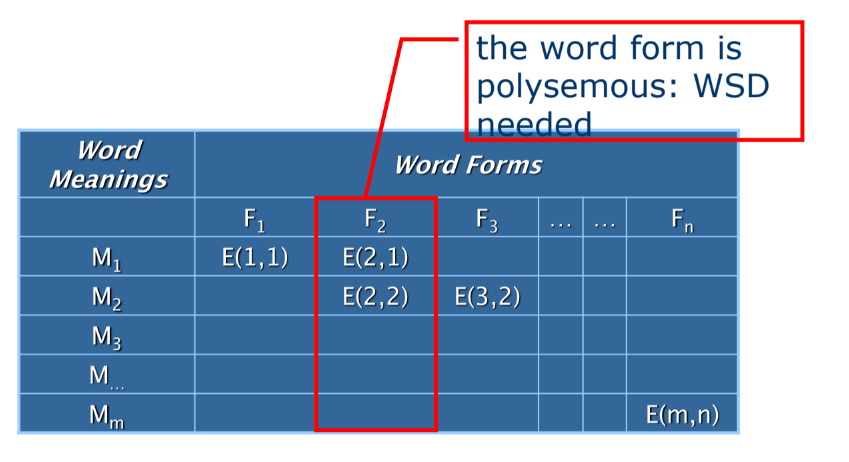
\includegraphics[scale=0.5]{assets/lex-mat-pol.png}
	\end{center}

	\subsection{Similarità semantica fra Synset}
	La similarità semantica fra synset è una misura di quanto due synset siano simili dal punto di vista semantico. Questa misura è utile per valutare la relazione tra due concetti e per stabilire quanto siano vicini in termini di significato. Esistono diverse metriche per calcolare la similarità semantica tra synset.
	
	\subsubsection{Similarità di Leacock-Chodorow}
	Un primo metodo è quello di \textbf{Leacock-Chodorow} si basa sul numero di nodi che separano i due synset nella gerarchia. La similarità è calcolata come:
	\begin{algorithm}[H]
		\caption{SinSim(a,b)}
		\begin{algorithmic}
			\State $N_p \leftarrow$ the number of nodes in path p from a to b
			\State D $\leftarrow$ the maximum depth of the taxonomy (in WordNet D = 16)
			\State \Return $- \log \left( \frac{N_p}{2 \cdot D} \right)$
		\end{algorithmic}
	\end{algorithm}
	Numero più grande indica maggiore similarità.

	\chapter{Relevance Feedback e Query Expansion}
	\section{Relevance Feedback}
	Il \textbf{relevance feedback} è una tecnica utilizzata nei motori di ricerca per migliorare la precisione dei risultati di una query. Consiste nell'ottenere un feedback dall'utente riguardo ai risultati restituiti e utilizzare queste informazioni per raffinare la query e migliorare i risultati futuri. Il relevance feedback è particolarmente utile quando i risultati iniziali non sono soddisfacenti o quando l'utente desidera ottenere risultati più rilevanti. Formulare una buona query per ottenere rilevanza maggiore quando non si conosce bene la collezione potrebbe essere complicato, di conseguenza il processo di raffinamento deve essere iterato.
	\vspace{\baselineskip}\\
	Il processo di raffinamento della query può essere effettuato in due principali metodi:
	\begin{itemize}
		\item \textbf{Relevance Feedback Esplicito}: l'utente fornisce un feedback esplicito sui risultati restituiti, indicando quali documenti sono rilevanti e quali non lo sono. Questo feedback viene utilizzato per aggiornare la query e migliorare i risultati futuri.
		\item \textbf{Relevance Feedback Implicito}: il sistema di ricerca analizza il comportamento dell'utente, ad esempio quali documenti vengono aperti, quanto tempo viene trascorso su ciascun documento, quali link vengono cliccati, ecc. Queste informazioni vengono utilizzate per inferire la rilevanza dei documenti e migliorare i risultati della query.
	\end{itemize}

	\subsection{Centroide}
	Il \textbf{centroide} è il centro di massa di un insieme di punti nello spazio vettoriale. In un contesto di recupero dell'informazione, il centroide è utilizzato per rappresentare il concetto di rilevanza di una query. Il centroide è calcolato come la media dei vettori dei documenti rilevanti. Il centroide è calcolato come:
	\[
	\overrightarrow{\mu}(C) = \frac{1}{|C|} \sum_{d \in C} \overrightarrow{d}
	\]
	dove \( C \) è l'insieme dei documenti e \( \overrightarrow{d} \) è il vettore del documento \( d \).
	\vspace{\baselineskip}\\
	Di base, il centroide non è normalizzato

	\subsection{Algoritmo di Rocchio}
	L'\textbf{algoritmo di Rocchio} utilizza il modello a spazi vettoriali per raffinare una query basandosi sul relevance feedback, andando a separare i documenti rilevanti da quelli non rilevanti.
	Dati:
	\begin{itemize}
		\item $D_r$: insieme dei documenti rilevanti tra tutti i documenti ottenuti
		\item $N_r$: numero dei documenti in $D_r$
		\item $D_n$: insieme dei documenti non rilevanti tra tutti i documenti ottenuti
		\item $N_n$: numero dei documenti in $D_n$
		\item $C_r$: insieme dei documenti rilevanti tra tutta la collezione di documenti
		\item $N:$ numero totale di documenti nella collezione
		\item $\alpha, \beta, \gamma$: parametri di pesatura
	\end{itemize}
	si ha che:
	\[
		\overrightarrow{q_{opt}} = \frac{1}{|C_r|} \sum_{\overrightarrow{d_j} \in C_r} \overrightarrow{d_j} - \frac{1}{N - |C_r|} \sum_{\overrightarrow{d_j} \in C_r} \overrightarrow{d_j}
	\]
	In questo modo otteniamo una query ottimale, ideale, che mi aspetto nel caso in cui si conosca l'insieme dei documenti rilevanti. Il problema è che questo insieme non è conosciuto ma verrà calcolato iterativamente. Potremmo formulare una query iniziale con la quale otterrei un feedback con il quale allontanare la query dai documenti non rilevanti e avvicinandola a quelli rilevanti.
	\vspace{\baselineskip}\\
	Nella pratica, l'algoritmo di Rocchio è calcolato come:
	\[
		\overrightarrow{q_m} = \alpha \overrightarrow{q_0} + \frac{\beta}{N_r} \sum_{\overrightarrow{d_j} \in D_r} \overrightarrow{d_j} - \frac{\gamma}{N_n} \sum_{\overrightarrow{d_j} \in D_n} \overrightarrow{d_j}
	\]
	dove $\overrightarrow{D_r}$ corrisponde al vettore di $D_r$ e $\overrightarrow{D_n}$ corrisponde al vettore di $D_n$. Questi due sono differenti da $C_r$. $q_m$ è la query modificata, $q_0$ è la query iniziale. $\alpha, \beta, \gamma$ sono parametri di pesatura scelti empiricamente o tramite processo di ottimizzazione.
	\begin{center}
		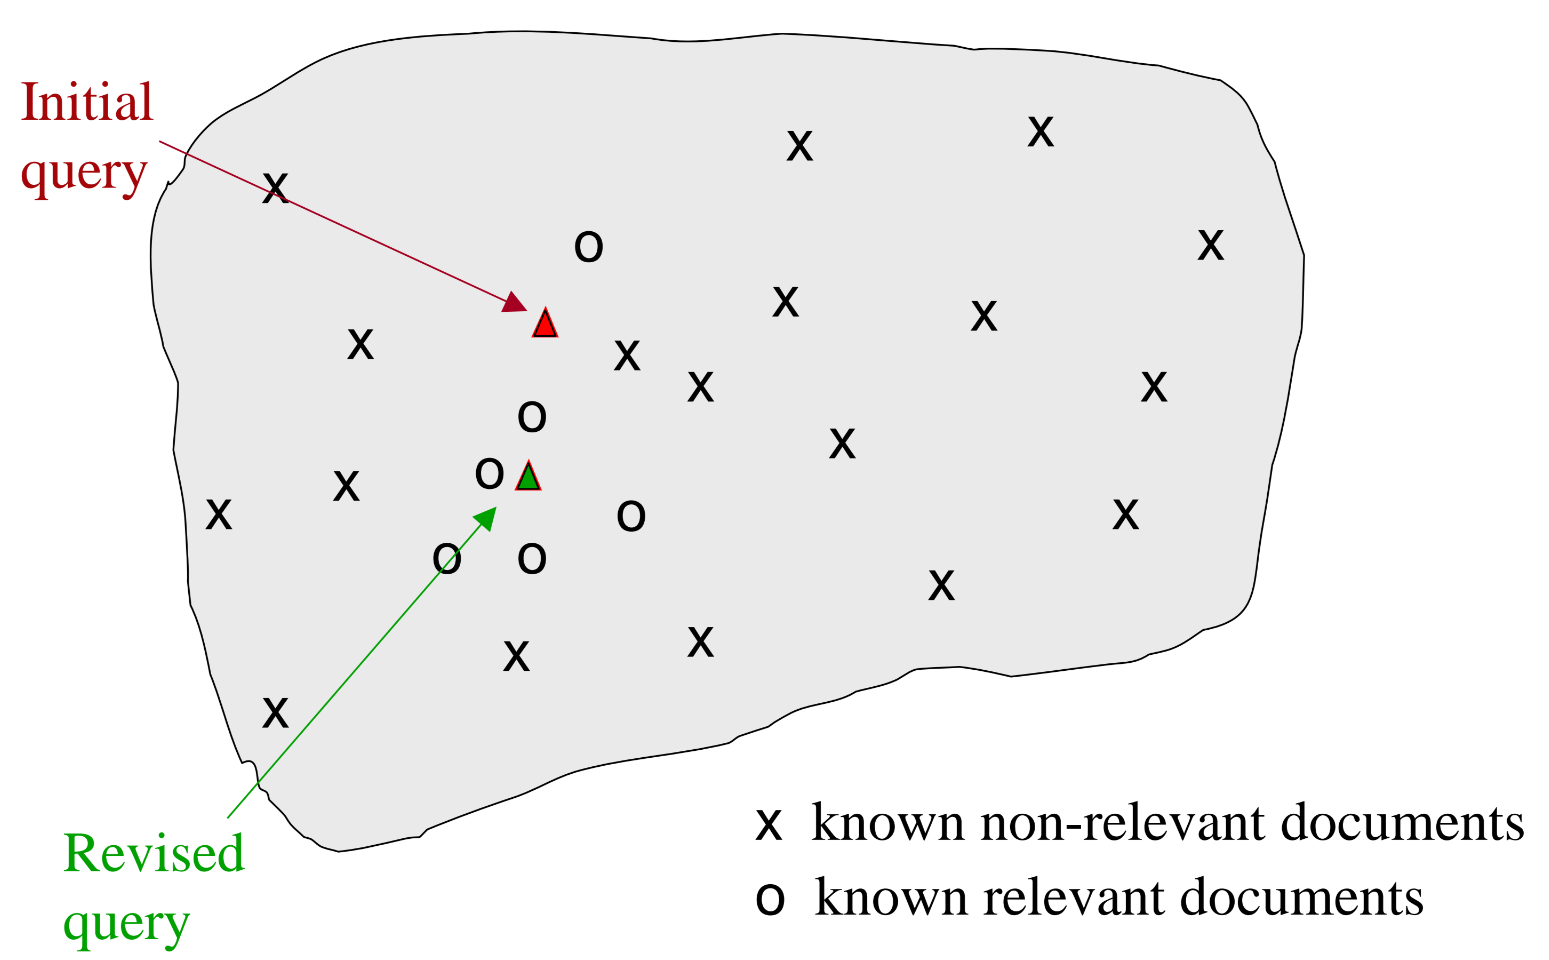
\includegraphics[scale=0.25]{assets/rocchio.png}
	\end{center}

	\subsubsection{Dettagli e Ottimizzazioni}
	Per approfondire l'algoritmo di Rocchio, è utile considerare alcuni dettagli che possono migliorarne l'efficacia nei sistemi di recupero delle informazioni. Un aspetto importante riguarda il bilanciamento tra i pesi $\alpha$, $\beta$ e $\gamma$. In particolare, $\alpha$ rappresenta il peso attribuito alla query originale, $\beta$ il contributo dei documenti rilevanti e $\gamma$ quello dei documenti irrilevanti. Se disponiamo di un numero elevato di documenti già giudicati, risulta conveniente aumentare i valori di $\beta$ e $\gamma$, per dare maggiore importanza al feedback degli utenti. Inoltre, durante l'aggiornamento della query, può capitare che alcuni termini nel vettore di query abbiano pesi negativi: questi vengono solitamente ignorati, cioè impostati a zero, per evitare distorsioni nei risultati.
	Un'altra sottigliezza riguarda la differenza di valore tra feedback positivo e negativo. Il feedback positivo, cioè i documenti rilevanti, è considerato più prezioso rispetto a quello negativo, rappresentato dai documenti irrilevanti. Per questo motivo, si tende a scegliere un valore di $\gamma$ inferiore a $\beta$. Alcuni sistemi, addirittura, scelgono di limitarsi al solo feedback positivo, impostando $\gamma = 0$.

	\subsection{Problemi e Limitazioni}
	Il feedback di rilevanza nei sistemi di recupero informazioni presenta alcune difficoltà significative. Anzitutto, le query lunghe risultano inefficaci per i motori di ricerca, in quanto richiedono tempi di risposta elevati, rallentando l'esperienza dell'utente, e aumentano i costi di elaborazione del sistema di ricerca. Per mitigare questo problema, si può adottare una soluzione parziale: invece di ricalcolare il peso di tutti i termini della query, ci si può concentrare su quelli più importanti, come i primi 20 termini con la frequenza maggiore. Inoltre, un altro ostacolo è che gli utenti sono spesso riluttanti a fornire feedback esplicito. Questo può derivare da una mancanza di comprensione del processo o semplicemente dalla difficoltà di impegnarsi attivamente nel fornire indicazioni aggiuntive al sistema. C'è poi un problema di trasparenza del processo: una volta applicato il feedback di rilevanza, può risultare difficile comprendere le ragioni per cui un determinato documento è stato recuperato. Questo introduce complessità nella spiegabilità del sistema e può ridurre la fiducia dell'utente nei risultati ottenuti. Infine, bisogna considerare che le necessità informative dell’utente possono cambiare nel corso dell'interazione con il sistema. Questo significa che il feedback di rilevanza, basato sulle esigenze iniziali, potrebbe non essere più adatto, portando a risultati meno pertinenti.

	\subsection{Valutazione delle strategie di Relevance Feedback}
	Nella valutazione delle strategie di feedback di rilevanza, è comune utilizzare due tipi di query: una query iniziale, indicata come $q_0$, e una query modificata dopo il feedback, chiamata $q_m$. Entrambe sono usate per generare grafici di precisione e richiamo, che consentono di comprendere come il feedback influenzi la qualità dei risultati.
	Per valutare l’efficacia del feedback di rilevanza, si possono adottare due approcci principali. Il primo approccio prevede di eseguire la valutazione su tutti i documenti della collezione, inclusi quelli già giudicati rilevanti. Questo metodo porta spesso a miglioramenti significativi, poiché il sistema “impara” a posizionare più in alto i documenti rilevanti conosciuti. Tuttavia, questa strategia potrebbe portare a una visione distorta delle prestazioni reali del sistema, in quanto l'utente ha già accesso a queste informazioni e quindi il risultato è influenzato da questa “familiarità” con i documenti. Il secondo approccio, invece, utilizza solo i documenti della collezione residua, ovvero esclude quelli che sono stati già giudicati rilevanti. Anche se le misurazioni risultanti sono generalmente più basse rispetto a quelle ottenute con la query iniziale, questa strategia offre una valutazione più realistica, poiché riflette meglio una situazione in cui l'utente non ha ancora visto la maggior parte dei documenti. Questo approccio permette inoltre un confronto più valido delle performance relative, poiché minimizza l’effetto di "conoscenza precedente" sui risultati.
	Dal punto di vista pratico, gli studi empirici mostrano che un singolo ciclo di feedback di rilevanza è spesso sufficiente per migliorare sensibilmente i risultati di ricerca. Un secondo ciclo, sebbene a volte utile, generalmente porta solo a un incremento marginale nella qualità dei risultati.
	\vspace{\baselineskip}\\
	Un metodo considerato ancora più robusto per valutare l’efficacia del feedback di rilevanza prevede l’utilizzo di due collezioni di documenti separate, ognuna con le proprie valutazioni di rilevanza. In questo scenario, la collezione iniziale viene divisa casualmente in due parti. La query $q_0$, con il feedback dell'utente, viene applicata sulla prima collezione, mentre la query modificata $q_m$ viene poi eseguita sulla seconda collezione. Questo metodo consente di misurare l'efficacia del feedback in maniera indipendente e convalidare i risultati ottenuti su una collezione distinta, riducendo così ulteriormente il rischio di sovrastimare i miglioramenti.
	\vspace{\baselineskip}\\
	È importante tenere conto di alcuni aspetti critici quando si valuta l’efficacia del feedback di rilevanza. Un'autentica valutazione della sua utilità dovrebbe idealmente confrontarlo con altre tecniche che richiedano un tempo o un impegno comparabili da parte dell’utente. Ad esempio, anziché utilizzare il feedback di rilevanza, l’utente potrebbe scegliere di modificare e risottomettere manualmente la query, ottenendo comunque una potenziale ottimizzazione dei risultati. In molti casi, gli utenti potrebbero preferire rivedere la propria query piuttosto che impegnarsi a giudicare la rilevanza di ciascun documento, specialmente se il processo è oneroso o poco intuitivo. Di fatto, non esiste alcuna evidenza definitiva che il feedback di rilevanza rappresenti l’uso migliore del tempo dell'utente; per alcuni, la revisione e risottomissione della query potrebbe risultare più efficace e meno impegnativa.

	\section{Pseudo Relevance Feedback}
	Il \textbf{pseudo relevance feedback} è una tecnica utilizzata nei motori di ricerca per migliorare la precisione dei risultati di una query senza richiedere un feedback esplicito dall'utente, il  quale molte volte aumenta i tempi di elaborazione o è complicato da ottenere. Questa tecnica si basa sull'assunzione che i primi documenti restituiti da una query siano rilevanti e vengano utilizzati per raffinare la query stessa tramite algoritmi di relevance feedback (es. Rocchio). Nella media dei casi, questo metodo si è dimostrato efficace nel migliorare la qualità dei risultati, anche se non sempre è in grado di garantire un incremento significativo della precisione, soprattutto quando i primi risultati di una query sono tutti dei sottoargomenti della query stessa. Inoltre, più iterazioni possono causare un peggioramento della qualità dei risultati, poiché la query può diventare troppo specifica e limitare la ricerca di documenti rilevanti. 

	\section{Indirect Relevance Feedback}
	Per ovviare ai limiti del relevance feedback esplicito e dello pseudo relevance feedback, è possibile utilizzare l'\textbf{indirect relevance feedback}. Questa tecnica si basa sull'analisi del comportamento dell'utente durante la ricerca, ad esempio quali documenti vengono aperti, quanto tempo viene trascorso su ciascun documento, quali link vengono cliccati, ecc. Queste informazioni vengono utilizzate per inferire la rilevanza dei documenti e migliorare i risultati della query. Questo metodo ad oggi è parte dei principali metodi di machine-learned ranking.

	\section{Query Expansion}
	Se nel relevance feedback, l'utente forniva un feedback esplicito sui risultati restituiti in modo tale da raffinare la query, nella \textbf{query expansion} si cerca di migliorare la qualità della query stessa aggiungendo termini associabili a quelli già presenti nella query. Questa tecnica è particolarmente utile quando la query iniziale è troppo generica o ambigua, portando a risultati poco precisi. La query expansion può essere effettuata in diversi modi, ad esempio aggiungendo sinonimi, termini correlati o termini associati. Questi termini aggiuntivi possono essere ottenuti da risorse lessicali come WordNet o da thesaurus, oppure tramite un'analisi globale statica di tutti i documenti nella collezione derivando automaticamente delle co-occorrenze basandosi sul thesaurus, o tramite un'analisi locale dinamica sui documenti del result set.

	\section{Query Assist}
	Il \textbf{query assist} è una tecnica di query expansion che fornisce suggerimenti all'utente durante la digitazione della query. Questi suggerimenti possono essere basati su query precedenti, termini più frequenti o popolari, o termini correlati. Questa tecnica viene tipicamente effettuata tramite mining dei log delle query precedentemente effettuate.
	
	\newpage
	\section{Esercizi}
	\subsection*{Esercizio 1}
	\textbf{Calcolare la similarità fra vettori}
	Siano x e y vettori non normalizzati in uno spazio a N dimensioni. Siano x' e y' vettori normalizzati con qualche strategia di normalizzazione. Sia sim(x,y) la similarità del prodotto interno. Sia cossim(x,y) la similarità del coseno. 

	\subsubsection{Caso 1: Vettori non normalizzati}
	\[
		\begin{array}{l}
		d_1 = (5,1,2) \text{dove 5, 1 e 2 sono i counter dei termini}\\
		d_2 = (0,1,1)\\
		d = (1,2,1)\\\\
		sim(d,d_1) = 5 \cdot 1 + 1 \cdot 2 + 2 \cdot 1 = 9\\
		sim(d,d_2) = 0 \cdot 1 + 1 \cdot 2 + 1 \cdot 1 = 3
	\end{array}
	\]
	Abbiamo che $sim(d,d_1) > sim(d,d_2)$, quindi d è più simile a $d_1$ che a $d_2$.
	\[
	\begin{array}{l}
		cossim(d,d_1) = \frac{sim(d,d_1)}{\sqrt{|d||d_2|}} = \frac{9}{\sqrt{5^2 + 1^2 + 2^2} \cdot \sqrt{1^2 + 2^2 + 1^2}} = \frac{9}{\sqrt{180}} = 0.671\\
		cossim(d,d_2) = \frac{3}{\sqrt{6} \cdot \sqrt{2}} = \frac{3}{\sqrt{12}} = 0.866  
	\end{array}
	\]
	Abbiamo che $cossim(d,d_1) < cossim(d,d_2)$, quindi d è più simile a $d_2$ che a $d_1$.
	non è un problema che diversi metodi di similarità diano risultati diversi, in quanto sono calcolati in modo diverso. Proviamo a normalizzare i vettori per vedere se cambia qualcosa.

	\subsubsection{Caso 2: Vettori normalizzati}
	\[
	\begin{array}{l}
		d_1 = (5,1,2) \land |d_1| = \sqrt{5^2 + 1^2 + 2^2} = \sqrt{30}\\
		d_2 = (0,1,1) \land |d_2| = \sqrt{2}\\
		d = (1,2,1) \land |d| = \sqrt{6}\\\\
		d'_1 = \left( \frac{5}{\sqrt{30}}, \frac{1}{\sqrt{30}}, \frac{2}{\sqrt{30}} \right)\\
		d'_2 = \left( 0, \frac{1}{\sqrt{2}}, \frac{1}{\sqrt{2}} \right)\\
		d' = \left( \frac{1}{\sqrt{6}}, \frac{2}{\sqrt{6}}, \frac{1}{\sqrt{6}} \right)\\\\
		sim(d',d'_1) = \frac{5}{\sqrt{30}} \cdot \frac{1}{\sqrt{6}} + \frac{1}{\sqrt{30}} \cdot \frac{2}{\sqrt{6}} + \frac{2}{\sqrt{30}} \cdot \frac{1}{\sqrt{6}} = \frac{9}{\sqrt{6} \cdot \sqrt{30}} = \frac{9}{\sqrt{180}} = 0.671\\
		sim(d',d'_2) = 0 \cdot \frac{1}{\sqrt{2}} + \frac{1}{\sqrt{2}} \cdot \frac{2}{\sqrt{6}} + \frac{1}{\sqrt{2}} \cdot \frac{1}{\sqrt{6}} = \frac{3}{\sqrt{12}} = 0.866
	\end{array}
	\]

	Abbiamo che $sim(d',d'_1) < sim(d',d'_2)$, quindi d' è più simile a $d'_2$ che a $d'_1$.

	\subsubsection{Caso 3: vettori normalizzati con strategia del peso massimo}
	\[
	\begin{array}{l}
		d_1 = (5,1,2) \land |d_1| = \max(5,1,2) = 5\\
		d_2 = (0,1,1) \land |d_2| = \max(0,1,1) = 1\\
		d = (1,2,1) \land |d| = \max(1,2,1) = 2\\\\
		d'_1 = \left( \frac{5}{5}, \frac{1}{5}, \frac{2}{5} \right) \land |d'_1| = \sqrt{1^2 + \frac{1}{5}^2 + \frac{2}{5}^2} = \sqrt{\frac{6}{5}}\\
		d'_2 = \left( 0, \frac{1}{1}, \frac{1}{1} \right) \land |d'_2| = \sqrt{0^2 + 1^2 + 1^2} = \sqrt{2}\\
		d' = \left( \frac{1}{2}, \frac{2}{2}, \frac{1}{2} \right) \land |d'| = \sqrt{\frac{1}{2}^2 + 1 + \frac{1}{2}^2} = \sqrt{\frac{3}{2}}\\\\
		sim(d',d'_1) = 1 \cdot \frac{1}{2} + \frac{1}{5} \cdot 1 + \frac{2}{5} \cdot \frac{1}{2} = \frac{1}{2} + \frac{1}{5} + \frac{1}{5} = \frac{9}{10} = 0.90\\
		sim(d',d'_2) = 0 \cdot \frac{1}{2} + 1 \cdot 1 + 1 \cdot \frac{1}{2} = 1 + \frac{1}{2} = \frac{3}{2} = 1.5\\
		cossim(d',d'_1) = \frac{0.90}{\sqrt{\frac{6}{5}} \cdot \sqrt{\frac{3}{2}}} = \frac{0.90}{\sqrt{\frac{18}{10}}} = 0.671\\
		cossim(d',d'_2) = \frac{1.5}{\sqrt{2} \cdot \sqrt{\frac{3}{2}}} = \frac{1.5}{\sqrt{3}} = 0.866 
	\end{array}
	\]
	Otteniamo che $sim(d',d'_1) < sim(d',d'_2)$, quindi d' è più simile a $d'_2$ che a $d'_1$.
	%%finisci caso 4 da pdf esercizi similarità

	%%aggiungi esercizio sul relevance feedback
	%%aggiungi esercizi pdf 20 ottobre 2020
	%%aggiungi esercizi pdf 26 ottobre 2020

	\chapter{Valutazione orientata ai sistemi}
	La valutazione dei sistemi, dei modelli e degli algoritmi di ritrovamento delle informazioni è un aspetto fondamentale per misurare l'efficacia e l'efficienza di un sistema di ricerca. La valutazione è necessaria per confrontare le prestazioni di diversi sistemi, identificare i punti di forza e di debolezza e migliorare le prestazioni complessive. Esistono diversi metodi e metriche per valutare i sistemi di ricerca, ognuno con vantaggi e limitazioni specifiche, come per esempio la qualirà dei risultati, la velocità di risposta, la scalabilità, la facilità d'uso, ecc.
	\vspace{\baselineskip}\\
	D'altro canto, valutare un sistema di ricerca è un compito complesso poichè l'efficacia di un sistema di ricerca dipende da diversi fattori, tra i quali la rilevanza dei risultati. La rilevanza, a sua volta, non è un concetto binario, ma può variare. Tendenzialmente, la rilevanza è:
	\begin{itemize}
		\item soggettiva, in quanto dipende dalle preferenze e dal giudizio dell'utente
		\item contestuale, in quanto può variare a seconda del contesto, della situazione e dello stato dell'utente
		\item cognitiva, in quanto dipende dalla percezione e dal comportamento dell'utente
		\item dinamica, in quanto può cambiare nel tempo
		\item situazionale, in quanto dipende dalle esigenze dell'utente
	\end{itemize}

	\section{Paradigma di Cranfield}
	Un primo tentativo di valutare i sistemi di ricerca è stato il \textbf{paradigma di Cranfield}, sviluppato negli anni '50 e '60 presso l'Università di Cranfield in Inghilterra. Questo paradigma ha introdotto il concetto di valutazione sperimentale dei sistemi di ricerca, fornendo due metriche principali per valutare l'efficacia dei sistemi di ricerca: il precision ratio e il recall ratio. Il precision ratio misura la proporzione di documenti rilevanti tra quelli restituiti dal sistema, mentre il recall ratio misura la proporzione di documenti rilevanti tra quelli effettivamente presenti nella collezione. Tendenzialmente, la maggior parte delle ricerche non richiedono un alto recall, ma piuttosto un alto precision, in quanto gli utenti sono più interessati a ottenere risultati rilevanti piuttosto che a recuperare tutti i documenti rilevanti. 
	\vspace{\baselineskip}\\
	Il paradigma di Cranfield utilizza una collezione di riferimenti di test nella quale sono contenuti documenti, query e i giudizi di rilevanza associati (tipicamente basati sull'argomento o sul contenuto).
	\vspace{\baselineskip}\\
	Il paradigma attua una serie di esperimenti per valutare i sistemi di ricerca, misurando la precision e il recall dei risultati ottenuti. Nello specifico, nel paradigma di Cranfield:
	\begin{enumerate}
		\item si selezionano differenti strategie e sistemi di ritrovamento delle informazioni da paragonare
		\item si utilizzano i suddetti sistemi per produrre liste di ranking di documenti per ciascuna query
		\item si calcola l'efficienza di ogni strategia su ogni query nella collezione di test in funzione dei documenti rilevanti recuperati
		\item si calcola la media dei punteggi su ogni query per ottenere una valutazione complessiva di efficienza di ogni sistema
		\item (opzionale, per determinare il miglior approccio) si effettuano test statistici per determinare le differenze fra le efficienze dei sistemi
	\end{enumerate}

	\section{Human Label Corpus (Test Collection)}
	In questo modello di valutazione si utilizza un corpus di documenti in funzione dei quali si collezionano insiemi esigenze informative. Basandosi su queste esigenze, un gruppo di esperti giudica ed etichetta i documenti in base alla loro rilevanza. Tipicamente si assume che la rilevanza sia binaria, ovvero un documento è rilevante o non rilevante. Il problema principale di questo modello è che la rilevanza è soggettiva e può variare da persona a persona. Inoltre, la valutazione richiede tempo e risorse umane, rendendo il processo costoso e non sempre pratico.
	
	\section{Precision e Recall}
	Come già detto in precedenza, la precision e il recall sono due metriche fondamentali per valutare l'efficacia, la correttezza e la completezza di un sistema di ricerca. La precision è l'abilità di restituire i documenti con ranking più alto che sono di elevata rilevanza e misura la proporzione di documenti rilevanti tra quelli restituiti dal sistema:
	\[
		\text{Precision} = \frac{\text{Numero di documenti rilevanti restituiti}}{\text{Numero di documenti restituiti}} = \frac{TP}{TP + FP}
	\]
	Il recall, invece, è l'abilità di cercare tutti i documenti rilevanti nel corpus e misura la proporzione di documenti rilevanti tra quelli effettivamente presenti nella collezione:
	\[
		\text{Recall} = \frac{\text{Numero di documenti rilevanti restituiti}}{\text{Numero di documenti rilevanti nella collezione}} = \frac{TP}{TP + FN}
	\]
	\begin{center}
		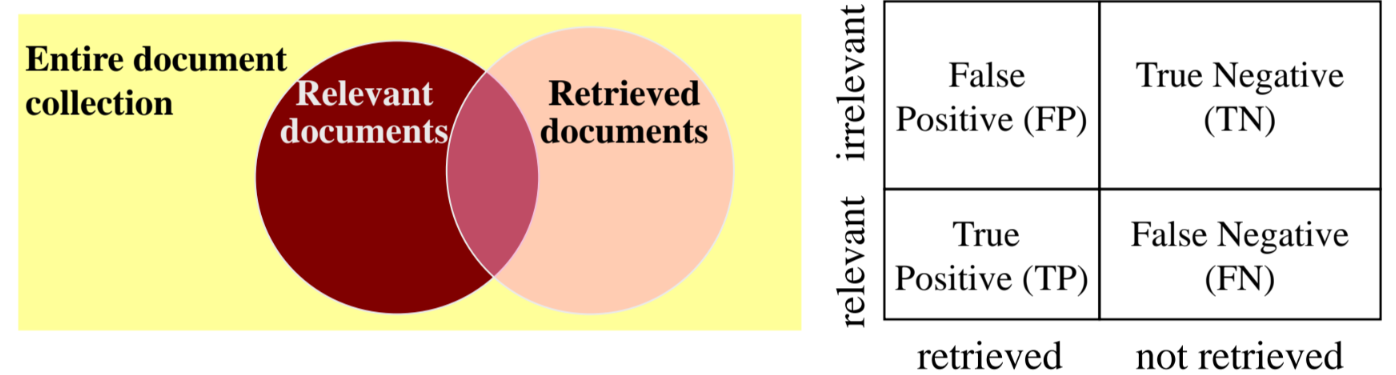
\includegraphics[scale=0.5]{assets/precision-recall.png}
	\end{center}
	Il recall è una funzione non decresente rispetto al numero di documenti recuperati poichè aumentando il numero di documenti recuperati, ad esempio di 1: se il documento aggiunto è rilevante allora TP aumenta di 1 e FN diminuisce di 1, se il documento aggiunto non è rilevante allora TP e FN rimangono invariati, FP aumenta di 1 e TN diminuisce di uno. In entrambi i casi il recall $\frac{TP}{TP + FN}$ non cambia. In un buon sistema, la precisione diminuisce all'aumentare del nuero di documenti recuperati o all'aumentare del recall.
	\begin{center}
		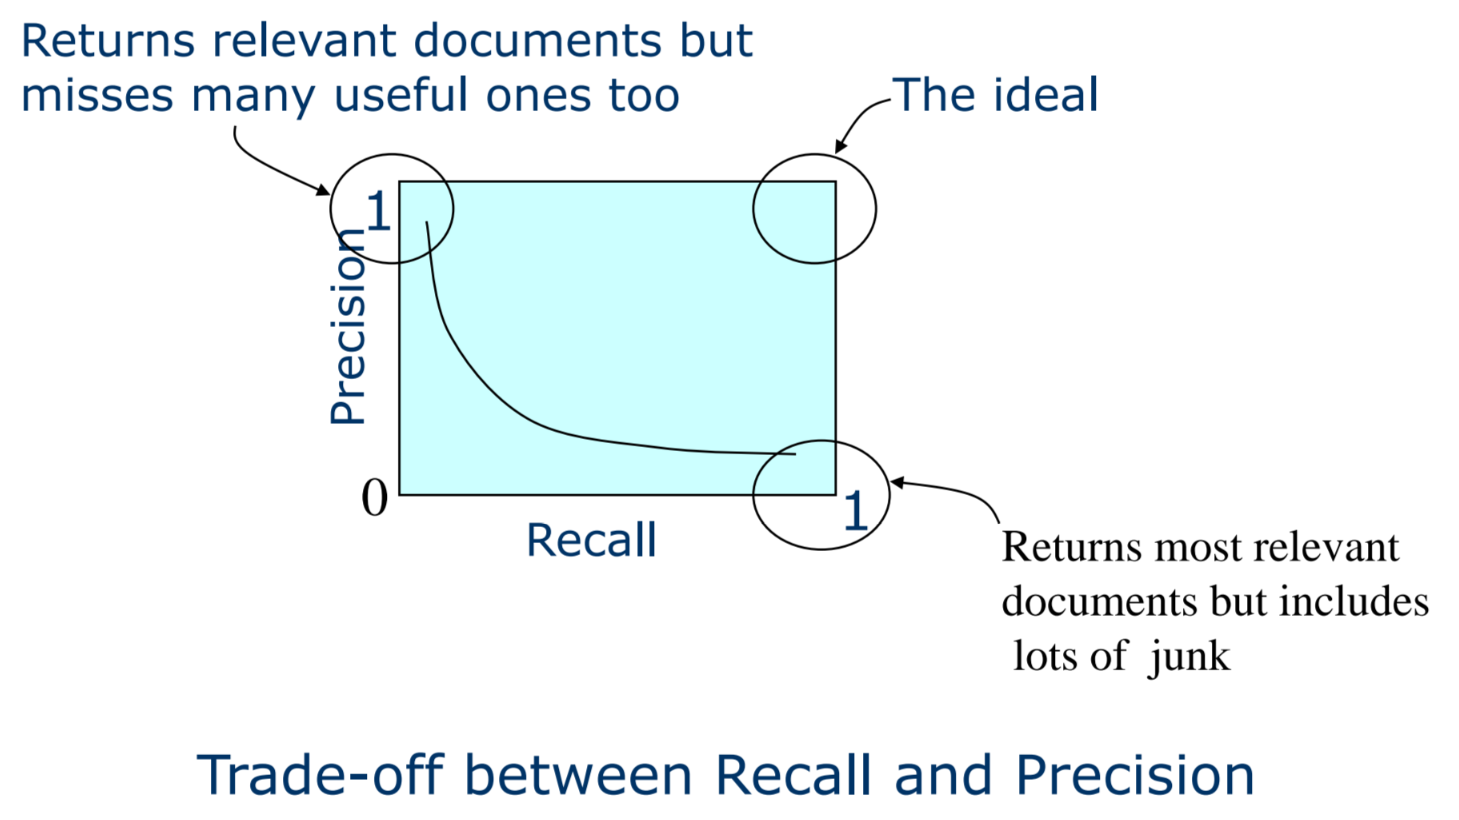
\includegraphics[scale=0.5]{assets/precision-vs-recall.png}
	\end{center}
	Determinare la metrica del recall spesso non è semplice poichè il numero totale di documenti rilevanti nella collezione non è sempre noto.
	%% difficoltà di precision e recall
	\section{Accuracy}
	Data una query, un motore di classificazione di documenti e un set di documenti. La \textbf{accuracy (accuratezza)} è la frazione di documenti classificati correttamente rispetto al totale dei documenti classificati:
	\[
		\text{Accuracy} = \frac{TP + TN}{TP + TN + FP + FN}
	\]
	
	\section{F1-Measure}
	Una misura per la valutazione della performance che combina precision e recall è la \textbf{F1-measure}, definita come la media armonica tra precision e recall:
	\[
		\text{F1-measure} = \frac{2 \cdot \text{Precision} \cdot \text{Recall}}{\text{Precision} + \text{Recall}} = \frac{2}{\frac{1}{\text{Precision}} + \frac{1}{\text{Recall}}}
	\]
	A differenza della media aritmetica, la media armonica ha bisogno che sia precision che recall siano alte per avere un valore alto. La F1-measure è particolarmente utile quando si ha bisogno di una metrica bilanciata tra precision e recall.

	\section{$F_{\beta}$-Measure (F-Measure parametrizzata)}
	La $F_{\beta}$-Measure è una generalizzazione della F1-measure che permette di dare più peso alla precision o al recall. La $F_{\beta}$-Measure è definita come:
	\[
		F_{\beta} = \frac{(1 + \beta^2) \cdot \text{Precision} \cdot \text{Recall}}{\beta^2 \cdot \text{Precision} + \text{Recall}} = \frac{(1 + \beta^2)}{\frac{\beta^2}{\text{Recall}} + \frac{1}{\text{Precision}}}
	\]
	che varia a seconda del valore di $\beta$:
	\begin{itemize}
		\item se $\beta = 1$, allora $F_{\beta} = F1$
		\item se $\beta > 1$, allora si dà più peso al recall
		\item se $\beta < 1$, allora si dà più peso alla precision
	\end{itemize}
	La E-Measure, invece, equivale a $1 - F_{\beta}$.

	\section{Curva di Precision-Recall}
	La curva di precision-recall è un grafico che mostra la relazione tra precision e recall al variare del numero di documenti recuperati. Questa curva è utile per valutare le prestazioni di un sistema di ricerca in modo più dettagliato rispetto a singole misure come precision e recall. In particolare, la curva di precision-recall permette di visualizzare come variano precision e recall al variare del numero di documenti restituiti. Un sistema ideale avrà una curva di precision-recall che si avvicina il più possibile all'angolo in alto a destra del grafico, indicando un alto valore sia di precision che di recall. La curva di precision-recall è particolarmente utile per confrontare diversi sistemi di ricerca e per identificare il trade-off tra precision e recall.
	\vspace{\baselineskip}\\
	Per determinare il punto all'interno del grafico, si posizionano sulle ascisse i valori di recall e sulle ordinate i valori di precision. 
	\begin{center}
		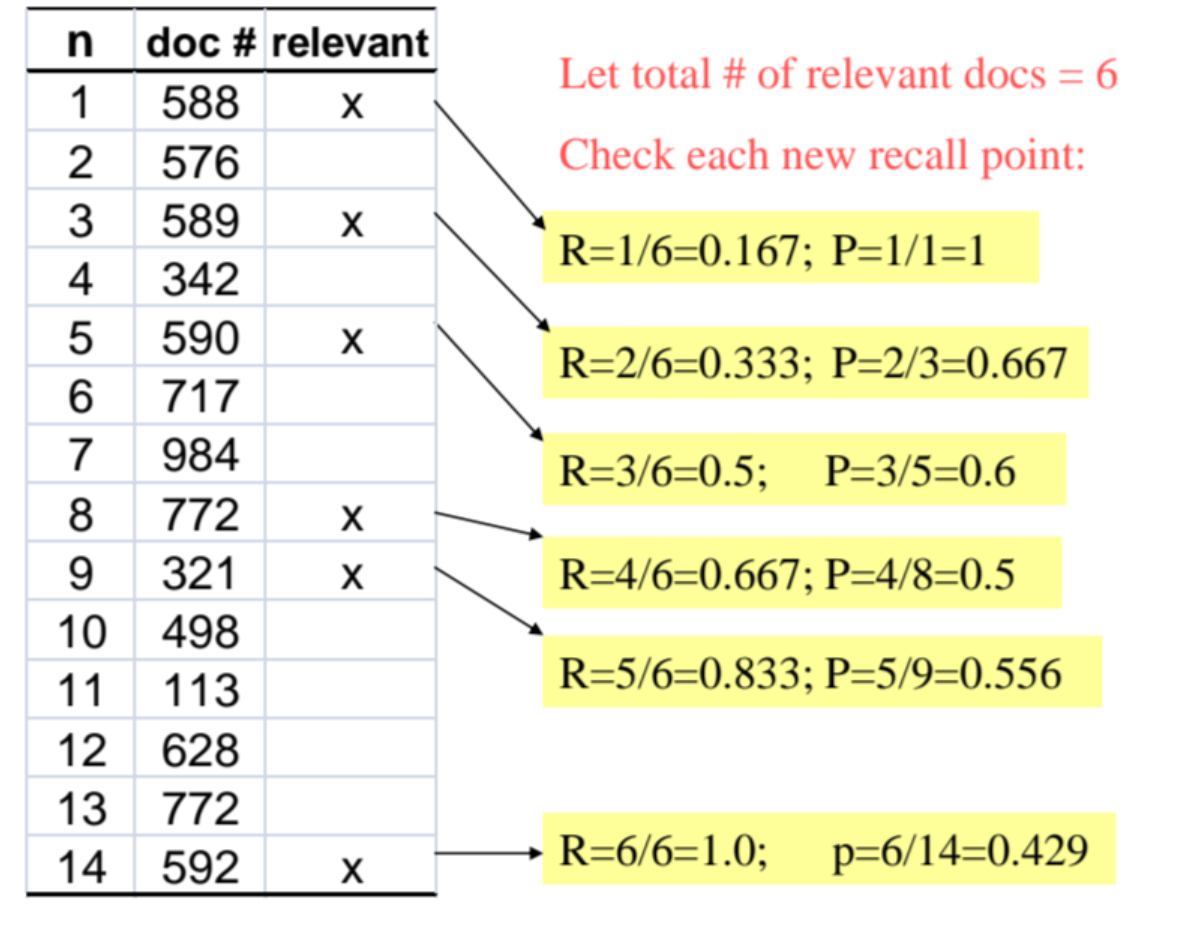
\includegraphics[scale=0.5]{assets/pre-rec-graph.png}
	\end{center}

	\subsection{Interpolazione della Curva di Precision-Recall}
	L'interpolazione della curva di precision-recall è un metodo utilizzato per valutare le prestazioni di un modello di classificazione, specialmente in contesti con classi sbilanciate. La precisione e il richiamo sono metriche fondamentali per misurare l'efficacia di un modello nel distinguere correttamente tra le classi. In questo contesto, l'interpolazione ha l'obiettivo di ottenere una rappresentazione più stabile e informativa della precisione a vari livelli di richiamo standard, riducendo così la variabilità dei valori di precisione su punti di richiamo discreti e rendendo la curva di precisione più "liscia".

	Per realizzare ciò, si fissano dei livelli di richiamo standard, come ad esempio \( r_j = \{0.0, 0.1, 0.2, \ldots, 1.0\} \). La precisione interpolata per ciascun livello di richiamo standard \( r_j \) è calcolata come il massimo valore di precisione ottenuto per tutti i livelli di richiamo \( r \) maggiori o uguali a \( r_j \), ovvero:
	
	\[
	P(r_j) = \max_{r_j \leq r} P(r)
	\]
	\begin{center}
		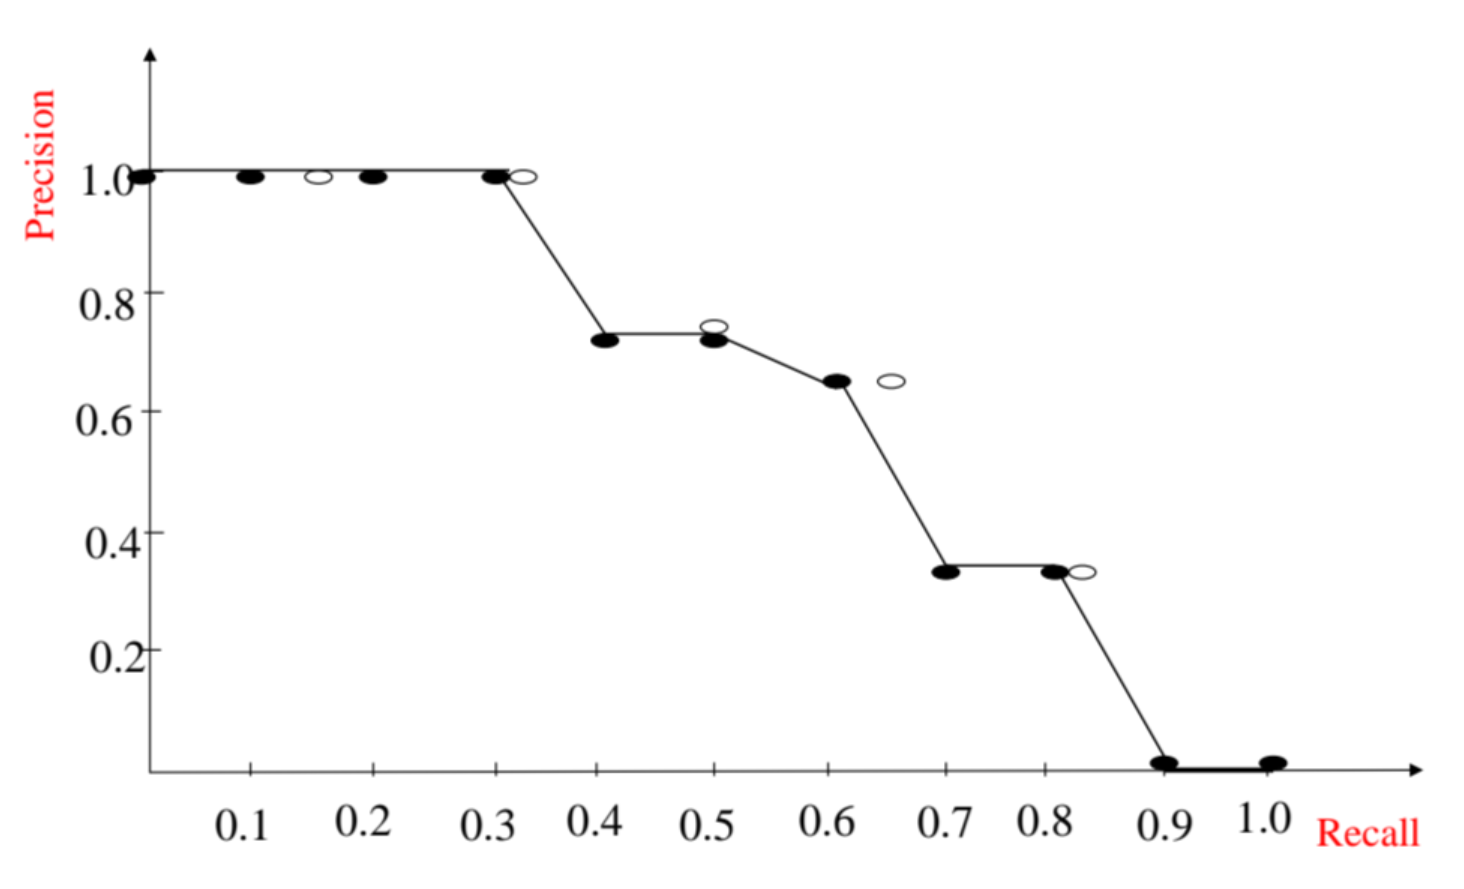
\includegraphics[scale=0.3]{assets/interpolated-pre-rec-graph.png}
	\end{center}

	\section{Precision @ k}
	La curva è un ottimo metodo per la valutazione dei sistemi di ricerca, ma può essere difficile da interpretare. Per questo motivo, spesso si utilizza la metrica \textbf{Precision @ k},che misura la precisione dei primi k documenti restituiti dal sistema. La Precision @ k è particolarmente utile quando si ha bisogno di valutare la qualità dei primi risultati restituiti da un sistema di ricerca. Ad esempio, se si ha bisogno di visualizzare solo i primi 10 risultati di una query, la Precision @ 10 è una metrica utile per valutare la qualità di questi risultati. La Precision @ k è definita come:
	\[
		\text{Precision @ k} = \frac{\text{Numero di documenti rilevanti tra i primi k restituiti}}{k}
	\]
	La precision@k ha diversi vantaggi. Ad esempio, è particolarmente adatta alle ricerche web, dove gli utenti tendono a considerare rilevanti solo i risultati che compaiono nelle prime pagine. Inoltre, permette di fissare un "cutoff" che aiuta a definire i risultati che il sistema deve considerare prioritari.
	Tuttavia, ci sono anche alcuni limiti. Primo, la precision@k non si presta bene alla media, poiché la scelta di k è arbitraria e può influenzare notevolmente i risultati complessivi. Inoltre, questo indicatore non distingue tra diversi ordinamenti di documenti con lo stesso numero di risultati rilevanti, trattandosi di una misura "set-based". Infine, la scelta di k può essere fuorviante per valutare le prestazioni del sistema, specialmente se il numero di documenti rilevanti è inferiore a k. In tal caso, la precision@k non potrà mai raggiungere il valore massimo di 1, anche con un sistema perfetto.

	\section{Average Precision}
	La \textbf{Average Precision (AP)} è una misura utilizzata per valutare l’efficacia di un sistema di recupero delle informazioni, come un motore di ricerca, nel posizionare i documenti rilevanti tra i primi risultati. Questa misura non si limita a contare quanti documenti rilevanti sono stati recuperati, ma tiene conto anche dell’ordine con cui appaiono nella lista dei risultati: l’obiettivo è che i documenti più pertinenti siano tra i primi, in modo da offrire un’esperienza più utile all’utente. L’Average Precision è calcolata come la media delle precisioni calcolate ad ogni punto in cui un documento rilevante nella collezione è recuperato. Nello specifico, l’Average Precision è definita come:
	\[
		\text{AP} = \frac{\sum_{k=1}^{m} Precision(p=k)}{m}
	\]
	\begin{center}
		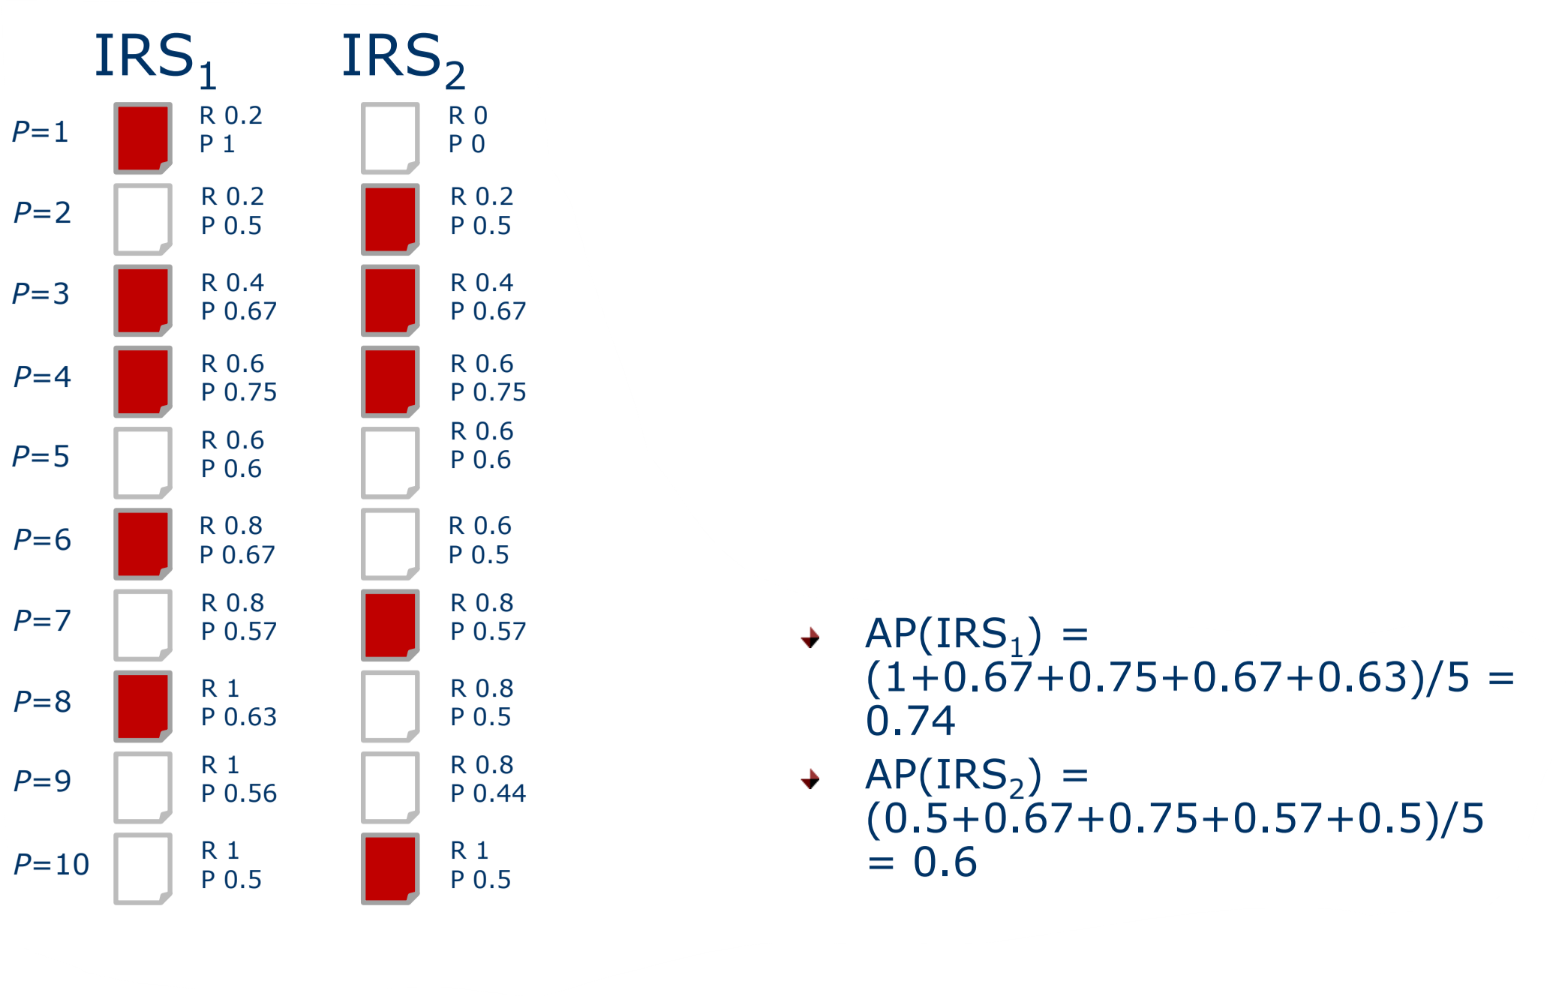
\includegraphics[scale=0.3]{assets/average-precision.png}
	\end{center}

	\section{Mean Average Precision (MAP)}
	La \textbf{Mean Average Precision (MAP)} è calcolata come la media delle Average Precision calcolate per ciascuna query nella collezione di test. Nello specifico, la Mean Average Precision è definita come:
	\[
		\text{MAP} = \frac{\sum_{i=1}^{n} \text{AP}_i}{n} = \frac{\sum_{1}^{n} \frac{\sum_{k=1}^{m} Precision(p=k)}{m}}{n}
	\]
	dove n è il numero totale di query e $m_j$ è il numero di documenti rilevanti per la query j.
	\begin{center}
		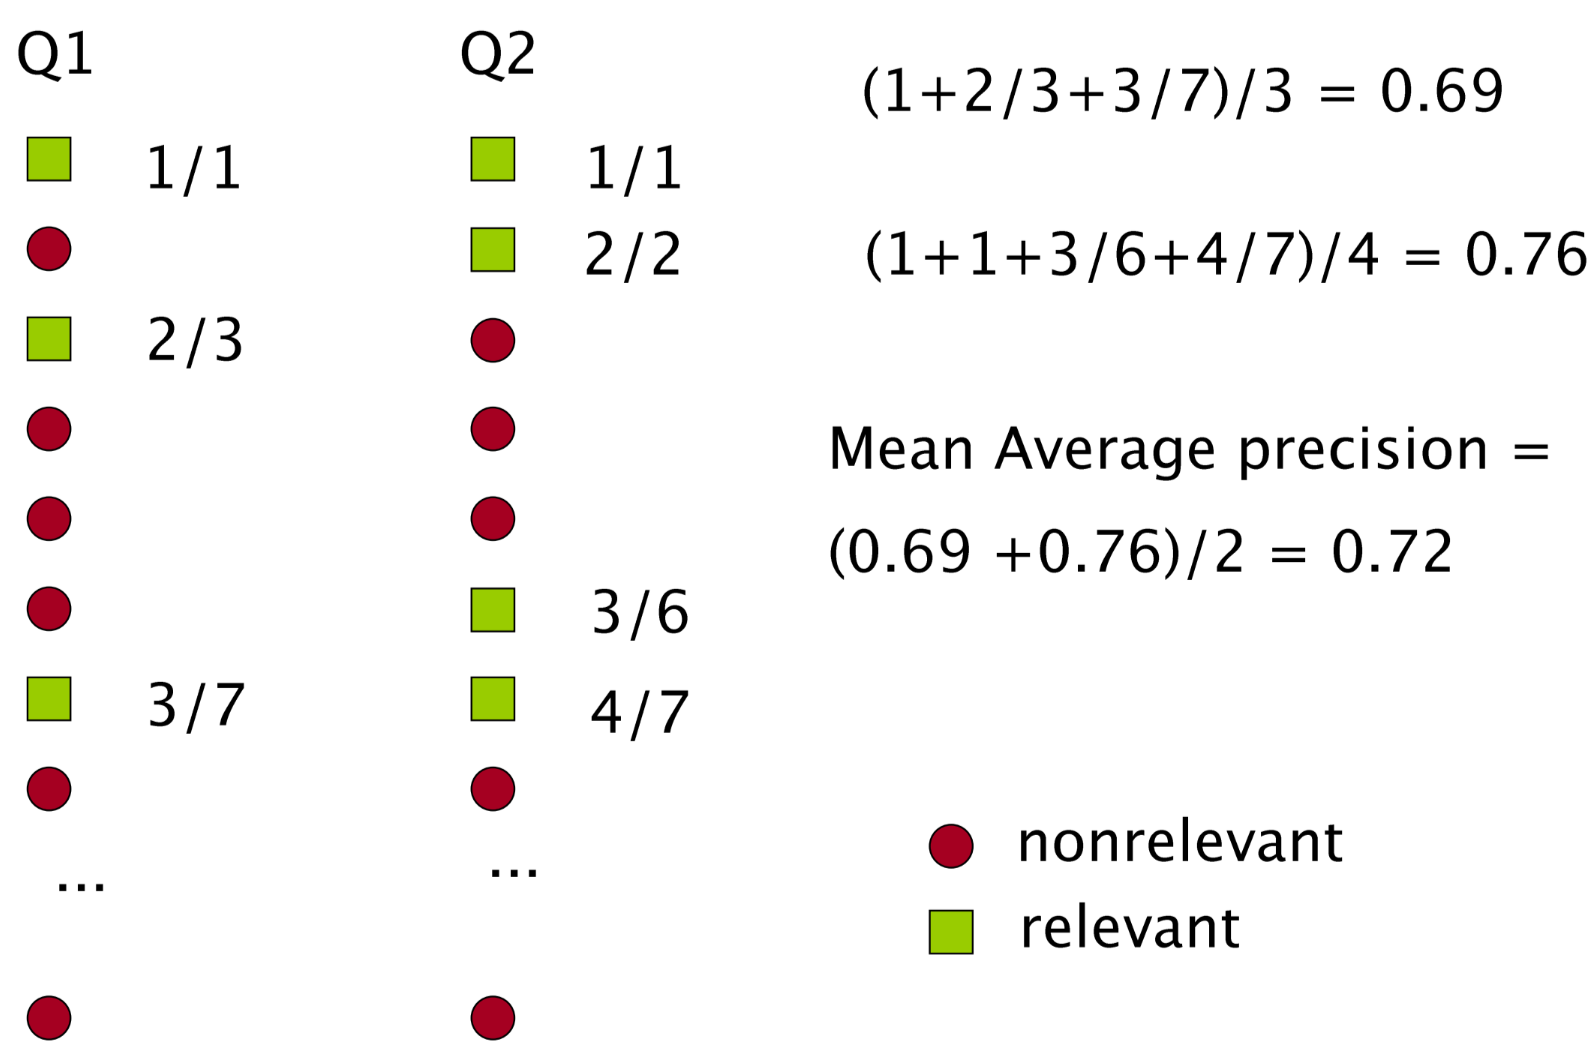
\includegraphics[scale=0.3]{assets/mean-average-precision.png}
	\end{center}

	\section{Geometric Mean Average Precision (GMAP)}
	La \textbf{Geometric Mean Average Precision (GMAP)} è una variante della Mean Average Precision che utilizza la media geometrica al posto della media aritmetica. La GMAP è particolarmente utile quando si hanno query complicate dove pochi documenti rilevanti vengono recuperati. In quest ametrica, valori piccoli hanno un impatto maggiore rispetto alla MAP. La GMAP è definita come:
	\[
		\text{GMAP} = \sqrt[n]{\prod_{i=1}^{n} \text{AP}_i}
	\]

	\section{R-Precision}
	La \textbf{R-Precision} è utile per osservare il comportamento di un algoritmo per le singole query. Misura la precisione alla posizione R, dove R è il numero di documenti rilevanti nella collezione. Un sistema perfetto avrà un R-Precision uguale a 1.
	\begin{center}
		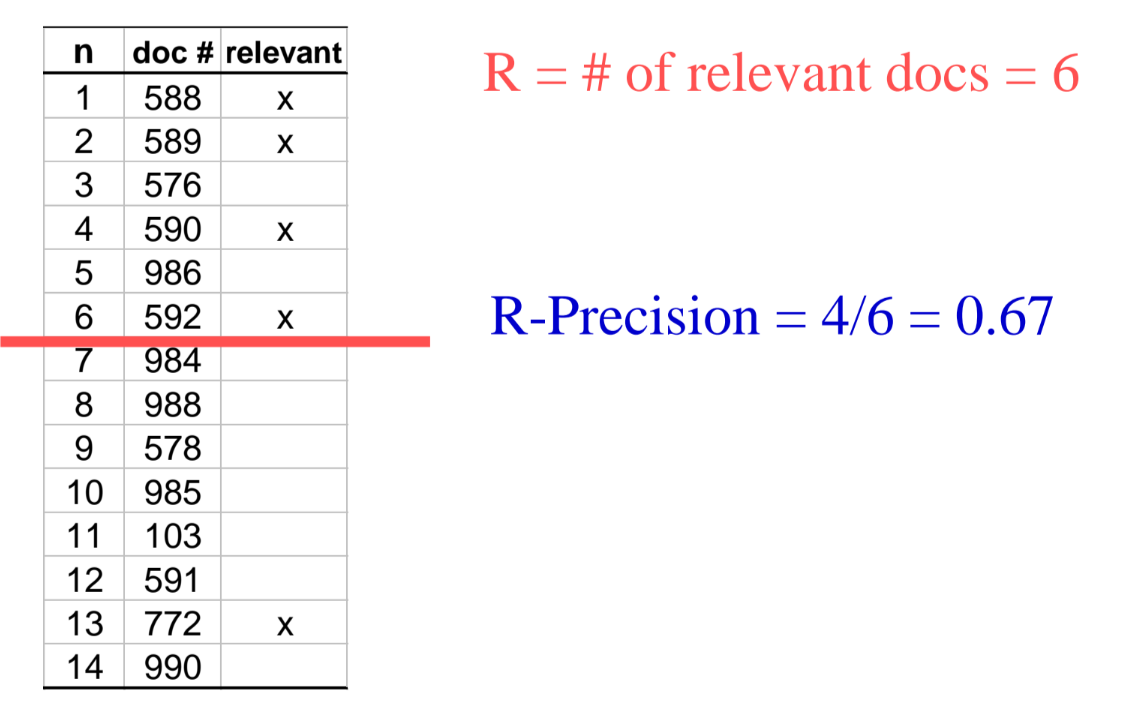
\includegraphics[scale=0.5]{assets/r-precision.png}
	\end{center}

	\section{Mean Reciprocal Rank (MRR)}
	La \textbf{Mean Reciprocal Rank (MRR)} è una metrica utilizzata per valutare l'efficienza dei motori di ricerca nel restituire documenti rilevanti in cima alla lista dei risultati. La MRR è definita come il reciproco della posizione del primo documento rilevante nella lista dei risultati. Nello specifico, la MRR è calcolata come:
	\[
		\text{MRR} = \frac{1}{|Q|} \sum_{i=1}^{|Q|} \frac{1}{\text{rank}_i}
	\]
	MRR è una buona metrica nei contesti in cui si ha bisogno di restituire la prima risposta corretta, come nei sistemi di QA (Question Answering) o nei sistemi di ricerca di documenti.  

	\section{Graded Non Binary Relevance}
	Finora abbiamo considerato la rilevanza come un concetto binario, ovvero un documento è rilevante o non rilevante, è ciò comportava l'impossibilità di distinguere tra documenti rilevanti di diverso grado. Tuttavia, spesso la rilevanza non è binaria, ma può variare in base al grado di rilevanza. In questi casi, si utilizzano metriche che tengono conto del grado di rilevanza nelle quali un documento viene giudicato per la sua rilevanza su una scala di valutazione. 

	\subsection{Discounted Cumulative Gain (DCG)}
	Il \textbf{Discounted Cumulative Gain (DCG)} è una metrica ampiamente utilizzata per valutare l'efficacia degli algoritmi di ranking, specialmente nei sistemi di Information Retrieval (IR). DCG si basa sul concetto di rilevanza graduata dei documenti, cioè sulla possibilità di assegnare a ciascun documento un punteggio di rilevanza su una scala. Quando si vanno ad esaminare i risultati di una query, possono essere condotte due osservazioni chiave per valutare la qualità dei risultati:
	\begin{itemize}
		\item i documenti con alto grado di rilevanza sono molto più utili di quelli con basso grado di rilevanza;
		\item più è bassa la posizione di ranking di un documento rilevante, meno è utile per l'utente poichè è meno probabile che venga visualizzato.
	\end{itemize}
	Supponiamo che i risultati delle query vengano valutati su una scala di valutazione da 0 a 3, dove 0 indica che il documento non è rilevante e 3 indica che il documento è altamente rilevante. Per query $q_1$ e $q_2$, supponiamo che i risultati siano i seguenti:
	\[
		\begin{array}{l}
			R_{q_1} = \{[d_3, 3], [d_5, 3], [d_9, 3], [d_{25}, 2], [d_{39}, 2], [d_{44}, 2], [d_{56}, 1], [d_{71}, 1], [d_{89}, 1], [d_{123},1]\}\\
			R_{q_2} = \{[d_3, 3], [d_{56}, 2], [d_{129}, 1]\}
		\end{array}
	\]
	Ricordiamo il ranking per la query $q_1$:
	\begin{multicols}{3}
		\begin{enumerate}
			\item $d_{123}$
			\item $d_{84}$
			\item $d_{56}$
			\item $d_{6}$
			\item $d_{8}$
			\item $d_{9}$
			\item $d_{511}$
			\item $d_{129}$
			\item $d_{187}$
			\item $d_{25}$
			\item $d_{38}$
			\item $d_{48}$
			\item $d_{250}$
			\item $d_{113}$
			\item $d_{3}$
		\end{enumerate}
	\end{multicols}
	Ricordiamo il ranking per la query $q_2$:
	\begin{multicols}{3}
		\begin{enumerate}
			\item \( d_{425} \)
			\item \( d_{87} \)
			\item \( d_{56} \)
			\item \( d_{32} \)
			\item \( d_{124} \)
			\item \( d_{615} \)
			\item \( d_{512} \)
			\item \( d_{129} \)
			\item \( d_{4} \)
			\item \( d_{130} \)
			\item \( d_{193} \)
			\item \( d_{715} \)
			\item \( d_{810} \)
			\item \( d_{5} \)
			\item \( d_{3} \)
		\end{enumerate}
		\end{multicols}
	Un modo per rappresentare questi punteggi di rilevanza per le prime posizioni nella lista dei risultati è attraverso il \textbf{vettore dei guadagni (Gain Vector, G)}. Questo vettore contiene i punteggi di rilevanza ordinati in base alla posizione dei documenti nel ranking, indicando quanto siano rilevanti i documenti nelle prime posizioni. Ad esempio, per q1 e q2, i vettori dei guadagni possono essere rappresentati rispettivamente come:
	\[
		\begin{array}{l}
			G_{q_1} = (1,0,1,0,0,3,0,0,0,2,0,0,0,0,3)\\
			G_{q_2} = (0,0,2,0,0,0,0,1,0,0,0,0,0,0,3)
		\end{array}
	\]
	Andando a sommare i guadagni ad ogni posizione nel ranking, otteniamo il \textbf{Cumulative Gain (CG)}. Per la query 1, per esempio il CG nella prima posizione è 1, nella seconda posizione è 1+0, nella terza posizione è 1+0+1, e così via. Il CG per q1 e q2 è rispettivamente:
	\[
		\begin{array}{l}
			CG_{q_1} = (1,1,2,2,2,5,5,5,5,7,7,7,7,7,10)\\
			CG_{q_2} = (0,0,2,2,2,2,2,3,3,3,3,3,3,3,6)
		\end{array}
	\]
	Formalmente, dati i gain vector $G_j$ per la query $q_j$, il Cumulative Gain $CG_j$ è definito come:
	\begin{equation}
		CG_j[i] =
		\begin{cases}
		  G_j[1] & \text{se } i = 1\\
		  G_j[i] + CG_j[i-1] & \text{se } i > 1
		\end{cases}
	\end{equation} 
	dove $CG_j[i]$ rappresenta il guadagno cumulativo fino alla posizione i-esima nel ranking.
	\vspace{\baselineskip}\\
	Tenendo conto della seconda osservazione chiave, ovvero che i documenti rilevanti nelle posizioni più basse sono meno utili, si introduce il \textbf{Discounted Cumulative Gain (DCG)}. Il DCG è una metrica che penalizza i documenti rilevanti nelle posizioni più basse, assegnando loro un punteggio inferiore rispetto ai documenti rilevanti nelle posizioni più alte. Il DCG è definito come:
	\[
		DCG_j[i] =
		\begin{cases}
		  G_j[1] & \text{se } i = 1\\
		  \frac{G_j[i]}{log_2i} + DCG_j[i-1] & \text{se } i > 1
		\end{cases}
	\]
	dove $DCG_j[i]$ rappresenta il guadagno cumulativo scontato fino alla posizione i-esima nel ranking per la query $q_j$.
	Per esempio, il DCG per q1 e q2 è rispettivamente:
	\[
		\begin{array}{l}
			DCG_{q_1} = (1,1,1.6,1.6,1.6,2.8,2.8,2.8,2.8,3.4,3.4,3.4,3.4,3.4,4.2)\\
			DCG_{q_2} = (0,0,1.3,1.3,1.3,1.3,1.3,1.6,1.6,1.6,1.6,1.6,1.6,1.6,2.4)
		\end{array}
	\]
	\subsection{DCG Curves}
	La curva DCG è un grafico che mostra il guadagno cumulativo scontato al variare del numero di documenti recuperati. Questa curva è utile per valutare l'efficacia degli algoritmi di ranking, specialmente nei sistemi di Information Retrieval (IR). La curva DCG permette di visualizzare come varia il guadagno cumulativo scontato al variare del numero di documenti recuperati. Per produrre la curva CG e DCG su un set di query, è necessario mediare i valori di CG e DCG per ciascuna query.
	\vspace{\baselineskip}\\
	Dato un set di $N_q$ query, \textbf{Average $\overline{CG}[i]$} e \textbf{Average $\overline{DCG}[i]$} sono definiti come:
	\[
		\begin{array}{l}
			\text{Average } \overline{CG}[i] = \frac{1}{N_q} \sum_{j=1}^{N_q} CG_j[i] \\
			\text{Average } \overline{DCG}[i] = \frac{1}{N_q} \sum_{j=1}^{N_q} DCG_j[i]
		\end{array}
	\]
	Per esempio, i valori di Average $\overline{CG}[i]$ e Average $\overline{DCG}[i]$ per le query q1 e q2 sono rispettivamente:
	\[
		\begin{array}{l}
			\text{Average } \overline{CG}[i] = (0.5, 0.5, 2.0, 2.0, 2.0, 3.5, 3.5, 4.0, 4.0, 5.0, 5.0, 5.0, 5.0, 5.0, 8.0)\\
			\text{Average } \overline{DCG}[i] = (0.5, 0.5, 1.5, 1.5, 1.5, 2.1, 2.1, 2.2, 2.2, 2.5, 2.5, 2.5, 2.5, 2.5, 3.3)
		\end{array}
	\]
	Una volta calcolati i valori di Average $\overline{CG}[i]$ e Average $\overline{DCG}[i]$, è possibile rappresentarli graficamente per ottenere la curva.

	\subsection{Ideal CG and DCG}
	Le misure di precisione e richiamo sono calcolate rispetto all'insieme dei documenti rilevanti, il che implica che possono essere utilizzate direttamente per confrontare diversi algoritmi. Tuttavia, le metriche di Cumulative Gain (CG) e Discounted Cumulative Gain (DCG), come definite in precedenza, non sono calcolate rispetto ad alcun baseline, il che rende problematico il loro uso diretto per comparare algoritmi di recupero distinti. Questo perché tali metriche non normalizzate potrebbero risultare fuorvianti. Una soluzione a questo problema è l'uso di metriche normalizzate, che richiedono la definizione di un baseline per effettuare la normalizzazione. Tale baseline è costituito dalle metriche ideali CG e DCG.

	\subsubsection{Definizione di CG e DCG Ideali}
	Consideriamo un insieme di test per una query $q$, dove i documenti rilevanti individuati dagli esperti sono suddivisi come segue: $n_3$ documenti hanno un punteggio di rilevanza pari a 3, $n_2$ documenti hanno un punteggio di 2, $n_1$ documenti un punteggio di 1 e i restanti documenti un punteggio di 0 (ovvero, considerati non rilevanti). 
	
	Il vettore ideale di guadagno (\textit{Ideal Gain}, IG) viene creato ordinando tutti i punteggi di rilevanza in ordine decrescente, ottenendo:
	\[
	IG = (3, \ldots, 3, 2, \ldots, 2, 1, \ldots, 1, 0, \ldots, 0).
	\]
	
	In altre parole, il vettore $IG$ è composto da $n_3$ punteggi di valore 3, seguiti da $n_2$ punteggi di valore 2, $n_1$ punteggi di valore 1, e infine i documenti non rilevanti con punteggio 0.
	
	Per esempio, per le query $q_1$ e $q_2$, avremo:
	\[
	IG_{q_1} = (3, 3, 3, 2, 2, 2, 1, 1, 1, 1, 1, 0, 0, 0, 0, 0),
	\]
	\[
	IG_{q_2} = (3, 2, 1, 0, 0, 0, 0, 0, 0, 0, 0, 0).
	\]
	
	\subsubsection{Calcolo degli ICG e IDCG}
	Dato il vettore $IG$, possiamo calcolare i vettori ideali CG ($ICG$) e ideali DCG ($IDCG$) analogamente a quanto fatto per il calcolo delle metriche CG e DCG standard. Ad esempio, per le query $q_1$ e $q_2$, i vettori ideali risultano essere:
	\[
	ICG_{q_1} = (3, 6, 9, 11, 13, 15, 16, 17, 18, 19, 19, 19, 19, 19, 19, 19),
	\]
	\[
	ICG_{q_2} = (3, 5, 6, 6, 6, 6, 6, 6, 6, 6, 6, 6).
	\]
	
	I corrispondenti vettori $IDCG$ sono calcolati come segue:
	\[
	IDCG_{q_1} = (3.0, 6.0, 7.9, 9.8, 10.5, 10.9, 11.2, 11.5, 11.8, 11.8, 11.8, 11.8, 11.8, 11.8, 11.8, 11.8),
	\]
	\[
	IDCG_{q_2} = (3.0, 5.0, 5.6, 5.6, 5.6, 5.6, 5.6, 5.6, 5.6, 5.6, 5.6, 5.6).
	\]
	
	\subsection{Media delle Metriche ICG e IDCG}
	Le medie delle metriche ideali possono essere calcolate come:
	\[
	ICG[i] = \frac{1}{N_q} \sum_{j=1}^{N_q} ICG_j[i], \quad IDCG[i] = \frac{1}{N_q} \sum_{j=1}^{N_q} IDCG_j[i].
	\]
	
	Ad esempio, per le query $q_1$ e $q_2$, i vettori medi sono:
	\[
	ICG = (3.0, 5.5, 7.5, 8.5, 9.5, 10.5, 11.0, 11.5, 12.0, 12.5, 12.5, 12.5, 12.5, 12.5, 12.5, 12.5),
	\]
	\[
	IDCG = (3.0, 5.5, 6.8, 7.3, 7.7, 8.1, 8.3, 8.4, 8.6, 8.7, 8.7, 8.7, 8.7, 8.7, 8.7, 8.7).
	\]
	
	Confrontando le curve medie di CG e DCG per un dato algoritmo con le curve ideali, possiamo comprendere quanto margine di miglioramento sia possibile. Le curve ideali rappresentano infatti la massima qualità di recupero ottenibile.
	
	\subsection{Normalizzazione della DCG}
	Sebbene le metriche di precisione e richiamo possano essere direttamente confrontate con una curva ideale che riflette una precisione del 100\% a tutti i livelli di richiamo, le metriche DCG non sono costruite rispetto a tale curva ideale. Anche se è possibile tracciare le curve ideali di DCG per comprendere la massima qualità di recupero, questo non facilita il confronto tra due algoritmi di ranking diversi. Per risolvere questo problema, è possibile normalizzare la metrica DCG come segue.
	\vspace{\baselineskip}\\
	Datie le curve di CG, ICG, DCG e IDCG mediati per un set di $N_q$ query, la CG e la DCG normalizzate sono definite come:
	\[
		NCG[i] = \frac{\overline{CG}[i]}{\overline{ICG}[i]}, \quad NDCG[i] = \frac{\overline{DCG}[i]}{\overline{IDCG}[i]}.
	\]
	Nel caso delle query $q_1$ e $q_2$, NCG e NDCG sono rispettivamente:
	\[
		\begin{array}{l}
			NCG = (0.17, 0.03, 0.27, 0.24, 0.21, 0.33, 0.32, 0.35, 0.33, 0.40, 0.40, 0.40, 0.40, 0.40, 0.64)\\
			NDCG = (0.17, 0.09, 0.21, 0.20, 0.19, 0.25, 0.26, 0
			26, 0.29, 0.29, 0.29, 0.29, 0.29, 0.29, 0.38)
		\end{array}
	\]
	Costruendo le curve NCG e NDCG, possiamo confrontare le aree sottostanti le curve di un algoritmo con quelle delle curve ideali per valutare l'efficacia del sistema di ranking. Più è alta l'area sottostante la curva, migliore è l'algoritmo di ranking.

	\subsection{Discussione sulle Metriche di Rilevanza Graduale}
	Le metriche \textit{Cumulative Gain} (CG) e \textit{Discounted Cumulative Gain} (DCG) mirano a prendere in considerazione valutazioni di rilevanza su più livelli, invece dei più comuni giudizi binari di rilevanza utilizzati nelle metriche di precisione e richiamo. Questo approccio ha il vantaggio di permettere di distinguere i documenti altamente rilevanti da quelli moderatamente rilevanti, poiché i primi ricevono punteggi di rilevanza più alti. Tuttavia, tra gli svantaggi intrinseci troviamo che le valutazioni su più livelli sono più difficili e dispendiose in termini di tempo da generare e sono soggette a errori dovuti alla soggettività nell'interpretazione dei punteggi di rilevanza multipli.
	Nonostante queste difficoltà, le metriche CG e DCG offrono diversi vantaggi:
	\begin{itemize}
		\item[(a)] consentono di combinare in modo sistematico i ranghi dei documenti e i punteggi di rilevanza;
		\item[(b)] il guadagno cumulato fornisce una singola metrica di qualità del recupero a qualsiasi posizione nella classifica, indipendentemente dal richiamo;
		\item[(c)] il guadagno cumulato evidenzia i benefici derivanti dai documenti rilevanti fino a una certa posizione nella classifica, rendendo così la metrica più resistente agli \textit{outlier};
		\item[(d)] il guadagno cumulato scontato consente di ridurre il peso dei documenti rilevanti posizionati più in basso nella classifica.
	\end{itemize}
	Pertanto, in situazioni in cui è richiesta un'elevata accuratezza di valutazione per confrontare algoritmi sofisticati e maturi con una qualità di recupero simile, le metriche CG e DCG offrono un'interessante alternativa alle metriche consolidate di precisione e richiamo.

	\section{Metriche di Correlazione dei Ranking}
	Le metiche di precision e recall permettono di effettuare una comparazione sulla rilevanza dei resultati di due o più sistemi di ranking. Tuttavia, possono verificarsi situazioni nelle quali non è possibile misurare la rilevanza e nelle quali è più determinante osservare la variazione di una funzione di ranking rispetto ad un'altra che si conosce essere corretta. In questi casi, è rilevante osservare e comparare l'ordine dei documenti rilevanti prodotto dai due sistemi. Per fare ciò, si utilizzano le metriche di correlazione dei ranking.
	\vspace{\baselineskip}\\
	Supponiamo $R_1$ e $R_2$ siano due sistemi di ranking. Una metrica di correlazione dei ranking produce un coefficiente di correlazione $C(R_1, R_2)$ che varia tra -1 e 1. Se il coefficiente è 1, i due ranking sono identici, se è -1, i due ranking sono in ordine inverso, se è 0, i due ranking sono indipendenti. All'aumentare del valore assoluto del coefficiente, i due ranking sono più simili.

	\subsection{Spearman's Rank Correlation Coefficient}
	Il \textbf{Coefficiente di correlazione di Spearman} è probabilmente la metrica più utilizzata per valutare la correlazione tra due ranking. Si basa sulla differenza tra le posizioni degli stessi documenti nei due ranking in esame. Sia $s_{1,j}$ la posizione del documento $d_j$ nel ranking $R_1$ e $s_{2,j}$ la posizione del documento $d_j$ nel ranking $R_2$. Un esempio di documenti e posizioni nei ranking è il seguente:
	\begin{table}[H]
		\centering
		\begin{tabular}{|c|c|c|c|c|}
			\hline
			\textbf{Document} & \textbf{$s_{1,j}$} & \textbf{$s_{2,j}$} & \textbf{$s_{1,j} - s_{2,j}$} & \textbf{$(s_{1,j} - s_{2,j})^2$}\\ 
			\hline
			$d_123$ & 1 & 2 & -1 & 1\\
			$d_84$ & 2 & 3 & -1 & 1\\
			$d_56$ & 3 & 1 & 2 & 4\\
			$d_6$ & 4 & 5 & -1 & 1\\
			$d_8$ & 5 & 4 & 1 & 1\\
			$d_9$ & 6 & 7 & -1 & 1\\
			$d_511$ & 7 & 8 & -1 & 1\\
			$d_129$ & 8 & 10 & -2 & 4\\
			$d_187$ & 9 & 6 & 3 & 9\\
			$d_25$ & 10 & 9 & 1 & 1\\
			\hline
			\multicolumn{4}{|c|}{Somma della distanza quadratica} & 24\\
			\hline
		\end{tabular}
	\end{table}
	Per produrre un risultato che va a rappresentare la qualità della correlazione tra i due ranking, si calcola la somma dei quadrati delle differenze tra le posizioni dei documenti nei due ranking.
	\vspace{\baselineskip}\\
	In generale, con K documenti rankati, il massimo valore della somma delle differenze quadrate è:
	\[
		\frac{K \times (K^2 - 1)}{3}
	\]
	Per calcolare il coefficiente di correlazione di Spearman, prendiamo prima in considerazione la seguente formula:
	\[
		\frac{\sum_{j=1}^{K} (s_{1,j} - s_{2,j})^2}{\frac{K \times (K^2 - 1)}{3}}
	\]
	che rappresenta la somma delle differenze quadrate divisa per il massimo valore possibile. Il suo valore sarà 0 se i due ranking sono identici, 1 se i due ranking sono completamente diversi. Se moltiplichiamo la frazione per 2, il valore possibile passa tra l'intervallo [0,2]. Per passare all'intervallo [-1,1], e quindi ricondurci all'idea generale di metrica di correlazione, sottraiamo 1 al risultato ottenuto. La formula finale per il coefficiente di correlazione di Spearman è:
	\[
		S(R_1, R_2) = 1 - \frac{6 \times \sum_{j=1}^{K} (s_{1,j} - s_{2,j})^2}{K \times (K^2 - 1)}
	\]
	Per i ranking $R_1$ e $R_2$ considerati in precedenza, il coefficiente di correlazione di Spearman è:
	\[
		S(R_1, R_2) = 1 - \frac{6 \times 24}{10 \times 99} = 1 - \frac{144}{990} = 1 - 0.145 = 0.854
	\]

	\subsection{Kendall's Tau Rank Correlation Coefficient}
	Nonostante l'ampio utilizzo e la semplicità di calcolo del coefficiente di correlazione di Spearman, risulta complicato assegnare una interpretazione in termini operativi al valore ottenuto. Per ovviare a questo problema, si utilizza il \textbf{coefficiente di correlazione di Kendall} il quale ha un'interpretazione più intuitiva e naturale.
	\vspace{\baselineskip}\\
	Quando pensiamo alla correlazione tra due ranking, ci aspettiamo che i documenti rilevanti siano posizionati in modo simile nei due ranking. Per esempio, consideriamo due documenti $d_j$ e $d_k$ e le loro posizioni nei ranking $R_1$ e $R_2$, e consideriamo la loro differenza di posizioni nei rank $s_{1,j} - s_{1,k}$ e $s_{2,j} - s_{2,k}$. Se entrambe le differenze sono positive o entrambe negative, allora i due documenti sono posizionati in modo coerente nei due ranking. Se una differenza è positiva e l'altra negativa, allora i due documenti sono posizionati in modo incoerente. 
	\vspace{\baselineskip}\\
	Consideriamo i primi 5 documenti della tabella precedente:
	\begin{table}
		\centering
		\begin{tabular}{|c|c|c|c|c|}
			\hline
			\textbf{Document} & \textbf{$s_{1,j}$} & \textbf{$s_{2,j}$} & \textbf{$s_{1,j} - s_{2,j}$} & \textbf{$s_{1,j} - s_{2,j}$}\\ 
			\hline
			$d_123$ & 1 & 2 & -1 & 1\\
			$d_84$ & 2 & 3 & -1 & 1\\
			$d_56$ & 3 & 1 & 2 & 4\\
			$d_6$ & 4 & 5 & -1 & 1\\
			$d_8$ & 5 & 4 & 1 & 1\\
			\hline
		\end{tabular}
	\end{table}
	Le coppie ordinate di documenti nel ranking $R_1$ sono:
	\[
		\begin{array}{l}
			(d_123, d_84), (d_123, d_56), (d_123, d_6), (d_123, d_8) \\
			(d_84, d_56), (d_84, d_6), (d_84, d_8) \\
			(d_56, d_6), (d_56, d_8) \\
			(d_6, d_8)
		\end{array}
	\]
	per un totale di 10 coppie ordinate. Le coppie ordinate di documenti nel ranking $R_2$ sono:
	\[
		\begin{array}{l}
			(d_56, d_123), (d_56, d_84), (d_56, d_8), (d_56, d_6) \\
			(d_123, d_84), (d_123, d_8), (d_123, d_6) \\
			(d_84, d_8), (d_84, d_6) \\
			(d_8, d_6)
		\end{array}
	\]
	Se andassimo a comparare le coppie ordinate nei due ranking marcando con C le coppie coerenti e con D le coppie incoerenti, otterremmo per i ranking $R_1$ e $R_2$ rispettivamente:
	\[
		\begin{array}{l}
			C, D, C, C\\
			D, C, C\\
			C, C\\
			D
		\end{array}
	\]
	\[
		\begin{array}{l}
			D, D, C, C\\
			C, C, C\\
			C, C\\
			D
		\end{array}
	\]
	Su un totale di 20 coppie ordinate, 14 sono coerenti e 6 sono incoerenti. Il coefficiente di correlazione di Kendall è definito come:
	\[
		\tau(R_1, R_2) = P(R_1 = R_2) - P(R_1 \neq R_2)
	\]
	dove $P(R_1 = R_2)$ è la probabilità che due documenti ordinati nei due ranking siano coerenti e $P(R_1 \neq R_2)$ è la probabilità che siano incoerenti. Per i ranking $R_1$ e $R_2$ considerati in precedenza, il coefficiente di correlazione di Kendall è:
	\[
		\tau(R_1, R_2) = \frac{14}{20} - \frac{6}{20} = 0.4
	\]
	Consideriamo $\delta(R_1, R_2)$ come il numero di coppie ordinate incoerenti nei due ranking e consideriamo $K(K-1) - \delta(R_1, R_2)$ come il numero di coppie ordinate coerenti. Allora:
	\[
		P(R_1 = R_2) = \frac{K(K-1) - \delta(R_1, R_2)}{K(K-1)}
	\]
	\[
		P(R_1 \neq R_2) = \frac{\delta(R_1, R_2)}{K(K-1)}
	\]
	che ci permette di riscrivere il coefficiente di correlazione di Kendall come:
	\[
		\tau(R_1, R_2) = 1 - 2 \times \frac{\delta(R_1, R_2)}{K(K-1)}
	\]
	Per i ranking $R_1$ e $R_2$ considerati in precedenza:
	\[
		\begin{array}{l}
			\delta(R_1, R_2) = 6\\
			K = 5 \\
			\tau(R_1, R_2) = 1 - 2 \times \frac{6}{5 \times (5-1)} = 1 - 2 \times \frac{6}{20} = 1 - 0.6 = 0.4
		\end{array}
	\]
	Il coefficiente di correlazione di Kendall è definito solo per ranking di uguale dimensione ed ha una struttura algebrica più semplice rispetto al coefficiente di correlazione di Spearman.


	\newpage
	\section{Esercizi}
	\subsection*{Esercizio 1 - Recall, Precision e F1}
	Sia q la query e supponiamo che nella collezione per q ci siano 5 documenti rilevanti.
	\vspace{\baselineskip}\\
	Siano $R_{1}(q)$ e $R_{2}(q)$ due sistemi da valutare. I risultati dei due sistemi sono:
	\begin{itemize}
		\item $R_{1}(q)$ restituisce 8 documenti, di cui 4 sono rilevanti
		\item $R_{2}(q)$ restituisce 5 documenti, di cui 3 sono rilevanti 
	\end{itemize}
	Calcoliamo la precision:
	\[
		\begin{array}{l}
			\text{Precision}_{R_{1}} = \frac{4}{8} = 0.5\\\\
			\text{Precision}_{R_{2}} = \frac{3}{5} = 0.6
		\end{array}
	\]
	Calcoliamo il recall:
	\[
		\begin{array}{l}
			\text{Recall}_{R_{1}} = \frac{4}{5} = 0.8\\\\
			\text{Recall}_{R_{2}} = \frac{3}{5} = 0.6
		\end{array}
	\]
	Calcoliamo l'F1 score:
	\[
		\begin{array}{l}
			\text{F1}_{R_{1}} = \frac{2 \cdot 0.5 \cdot 0.8}{0.5 + 0.8} = \frac{0.8}{1.3} = 0.615\\\\
			\text{F1}_{R_{2}} = \frac{2 \cdot 0.6 \cdot 0.6}{0.6 + 0.6} = \frac{0.72}{1.2} = 0.6
		\end{array}
	\]

	\subsection*{Esercizio 2 - Precision e Recall}
	Prendiamo invece i seguenti risultati:
	\begin{itemize}
		\item $R_{1}(q)$ restituisce 5 documenti, di cui 3 sono rilevanti (i primi 3)
		\item $R_{2}(q)$ restituisce 5 documenti, di cui 3 sono rilevanti (gli ultimi 3)
	\end{itemize}
	Calcoliamo la precision:
	\[
		\begin{array}{l}
			\text{Precision}_{R_{1}} = \frac{3}{5} = 0.6\\\\
			\text{Precision}_{R_{2}} = \frac{3}{5} = 0.6
		\end{array}
	\]
	Calcoliamo il recall:
	\[
		\begin{array}{l}
			\text{Recall}_{R_{1}} = \frac{3}{5} = 0.6\\\\
			\text{Recall}_{R_{2}} = \frac{3}{5} = 0.6
		\end{array}
	\]
	A parità di precision e recall, il sistema preferibile è $R_{1}$ in quanto restituisce i documenti rilevanti all'inizio della lista. Nonostante ciò, precision e recall non permettono di valutare esplicitamente la correttezza e la completezza di un sistema rispetto a un altro.

	\subsection*{Esercizio 3 - Interpolazione della Curva di Precision-Recall}
	Sia q la query e supponiamo che q abbia prodotto i seguenti risultati  RNRNRNNRRNNNNR. Supponiamo che il numero totale di documenti rilevanti sia 6. Andiamo a calcolare la precisione e il recall:
	\[
		\begin{array}{l}
			\text{R} \rightarrow P = 1, R = \frac{1}{6} = 0.167\\
			\text{N}\\
			\text{R} \rightarrow P = \frac{2}{3} = 0.667, R = \frac{2}{6} = 0.333\\
			\text{N}\\
			\text{R} \rightarrow P = \frac{3}{5} = 0.6, R = \frac{3}{6} = 0.5\\
			\text{N}\\
			\text{N}\\
			\text{R} \rightarrow P = \frac{4}{8} = 0.5, R = \frac{4}{6} = 0.667\\
			\text{R} \rightarrow P = \frac{5}{9} = 0.556, R = \frac{5}{6} = 0.833\\
			\text{N}\\
			\text{N}\\
			\text{N}\\
			\text{N}\\
			\text{R} \rightarrow P = \frac{6}{14} = 0.429, R = 1\\
			\end{array}
	\]
	Per effettuare l'interpolazione, fissiamo i livelli di richiamo standard $r_j = \{0.0, 0.1, 0.2, \ldots, 1.0\}$. Calcoliamo la precisione interpolata per ciascun livello di richiamo standard $r_j$:
	\begin{table}[H]
		\centering
		\begin{tabular}{|c|c|}
			\hline
			\textbf{Precision} & \textbf{Recall} \\ \hline
			1 & 0.0 \\ \hline
			1 & 0.1 \\ \hline
			1 & 0.167 \\ \hline
			0.667 & 0.2 \\ \hline
			0.667 & 0.3 \\ \hline
			0.667 & 0.333 \\ \hline
			0.6 & 0.4 \\ \hline
			0.6 & 0.5 \\ \hline
			0.556 & 0.6 \\ \hline
			0.5 & 0.667 \\ \hline
			0.556 & 0.7 \\ \hline
			0.556 & 0.8 \\ \hline
			0.556 & 0.833 \\ \hline
			0.429 & 0.9 \\ \hline
			0.429 & 1.0 \\ \hline
		\end{tabular}
	\end{table}

	\subsection*{Esercizio 4  - Traccia in Itinere 16/11/2023}
	Sia q una query che ha 6 documenti rilevanti nella collezione. Supponiamo che un algoritmo di ritrovamento riporti il seguente ranking R per la query q (R indica che il documento è rilevante; N indica che il documento è non rilevante; il risultato più a sinistra è il top della lista): R1: NRRNRNR.
	\begin{enumerate}
		\item Fornire la descrizione delle seguenti metriche: Precision, Recall, Average Precision, 
		R-precision, Reciprocal Rank
		\item Calcolare l’accuratezza del sistema di ritrovamento per q utilizzando le metriche al punto 1.  
		\item Riportare la curva di precision-recall per q, usando gli 11 livelli standard di recall 
	\end{enumerate}	
	1. Precision, recall, Average Precision, R-precision, Reciprocal Rank sono tutte metriche utilizzate per la valutazione della correttezza, completezza e qualità dei sistemi/metodi/algoritmi di ritrovamento delle informazioni. In particolare, la precision specifica la correttezza di un sistema e misura il numero di documenti rilevanti ritrovati sul numero di documenti ritrovati per la query q.
	\[
		\text{Precision} = \frac{\text{numero di documenti rilevanti ritrovati}}{\text{numero di documenti ritrovati}}
	\]
	La recall è la metrica che specifica la completezza di un sistema e misura il numero di documenti rilevanti nella collezione. 
	\[
		\text{Recall} = \frac{\text{numero di documenti rilevanti ritrovati}}{\text{numero di documenti rilevanti nella collezione}}
	\]
	L'average precision è una metrica che valutare l’efficacia di un sistema di recupero delle informazioni, come un motore di ricerca, nel posizionare i documenti rilevanti tra i primi risultati ed è calcolata come la media delle precisioni calcolate ad ogni punto in cui un documento rilevante nella collezione è recuperato.
	\[
		\text{AP} = \frac{\sum_{k=1}^{m} \text{Precision}(p=k)}{m}
	\]
	dove m è il numero totale di documenti rilevanti per la query q.\\
	La R-Precision è una metrica che misura la precisione alla posizione R, dove R è il numero di documenti rilevanti nella collezione. \\
	La Reciprocal Rank è una metrica che misura la posizione del primo documento rilevante nella lista dei risultati.
	\vspace{\baselineskip}\\
	2. Calcoliamo le metriche. Sono rilevanti 4 documenti su 7 ritrovati, quindi la precision è $\frac{4}{7} = 0.571$. La recall è $\frac{4}{6} = 0.667$. Per completezza calcolo anche la F1-Measure che misura la media armonica tra precision e recall: $F1 = \frac{2 \cdot 0.571 \cdot 0.667}{0.571 + 0.667} = 0.615$. Per calcolare l'average precision, vado prima a calcolare la precision per ogni documento ritrovato:
	\[
		\begin{array}{l}
			\text{N} \\
			\text{R} \rightarrow \frac{1}{2} = 0.5\\
			\text{R} \rightarrow \frac{2}{3} = 0.667\\
			\text{N} \\
			\text{R} \rightarrow \frac{3}{5} = 0.6\\
			\text{N} \\
			\text{R} \rightarrow \frac{4}{7} = 0.571\\
		\end{array}
	\]
	Calcoliamo l'average precision: $\text{AP} = \frac{0.5 + 0.667 + 0.6 + 0.571}{6} = 0.389$. Per calcolare la R-Precision,  calcoliamo la precisione ai primi 6 documenti ritrovati: $\frac{3}{6} = 0.5$. Infine, per calcolare la Reciprocal Rank, calcoliamo il reciproco della posizione del primo documento rilevante nella lista dei risultati: $\frac{1}{2} = 0.5$.
	\vspace{\baselineskip}\\
	Per riportare la curva di precision-recall, andiamo prima a calcolare precision e recall ad ogni documento rilevante ritrovato, successivamente si va a calcolare l'interpolazione della curva. 
	\[
		\begin{array}{l}
			\text{N}\\
			\text{R} \rightarrow P = \frac{1}{2} = 0.5, R = \frac{1}{6} = 0.167\\
			\text{R} \rightarrow P = \frac{2}{3} = 0.667, R = \frac{2}{6} = 0.333\\
			\text{N}\\
			\text{R} \rightarrow P = \frac{3}{5} = 0.6, R = \frac{3}{6} = 0.5\\
			\text{N}\\
			\text{R} \rightarrow P = \frac{4}{7} = 0.571, R = \frac{4}{6} = 0.667\\
		\end{array}
	\]
	Fissiamo i livelli di richiamo standard $r_j = \{0.0, 0.1, 0.2, \ldots, 1.0\}$. Calcoliamo la precisione interpolata per ciascun livello di richiamo standard $r_j$: $P(r_j) = \max_{\forall r \geq r_j} P(r)$.
	\begin{table}[h]
		\centering
		\begin{minipage}{0.45\textwidth}
			\centering
			\begin{tabular}{|c|c|}
				\hline
				\textbf{Precision} & \textbf{Recall} \\ \hline
				0.667 & 0.0 \\ \hline
				0.667 & 0.1 \\ \hline
				0.5 & 0.167 \\ \hline
				0.667 & 0.2 \\ \hline
				0.667 & 0.3 \\ \hline
				0.667 & 0.333 \\ \hline
				0.6 & 0.4 \\ \hline
				0.6 & 0.5 \\ \hline
				0.571 & 0.6 \\ \hline
				0.571 & 0.667 \\ \hline
				0 & 0.7 \\ \hline
				0 & 0.8 \\ \hline
				0 & 0.9 \\ \hline
				0 & 1.0 \\ \hline
			\end{tabular}
		\end{minipage}%
		\hfill
		\begin{minipage}{0.5\textwidth}
			\centering
			\begin{tikzpicture}
				\begin{axis}[
					xlabel={Recall},
					ylabel={Precision},
					ymin=0, ymax=1,
					xmin=0, xmax=1,
					grid=both,
					width=7cm, height=6cm,
					legend pos=south west,
					ylabel near ticks,
					xlabel near ticks
				]
				\addplot coordinates {
					(0.0, 0.667)
					(0.1, 0.667)
					(0.2, 0.667)
					(0.3, 0.667)
					(0.4, 0.6)
					(0.5, 0.6)
					(0.6, 0.571)
					(0.7, 0)
					(0.8, 0)
					(0.9, 0)
					(1.0, 0)
				};
				\end{axis}
			\end{tikzpicture}
		\end{minipage}
	\end{table}
	
	\subsection*{Esercizio 5 - 20 Novembre 2022}
	1. Calcolare il coefficiente di correlazione di Spearman e di Kendall tra i due ranking $R_{1}$ e $R_{2}$:
	\[
		\begin{array}{l}
			R_{1} = D2 D1 D4 D3\\
			R_{2} = D3 D4 D1 D2
		\end{array}
	\]
	Possiamo già notare che i due ranking sono in ordine inverso. Prevedo che il coefficiente di correlazione di Spearman sarà -1 e il coefficiente di correlazione di Kendall sarà 1.
	Per calcolare il coefficiente di correlazione di Spearman, calcoliamo la somma delle differenze quadrate tra le posizioni dei documenti nei due ranking:
	\begin{table}[H]
		\centering
		\begin{tabular}{|c|c|c|c|c|}
			\hline
			\textbf{Document} & \textbf{$s_{1,j}$} & \textbf{$s_{2,j}$} & \textbf{$s_{1,j} - s_{2,j}$} & \textbf{$(s_{1,j} - s_{2,j})^2$}\\ 
			\hline
			D1 & 2 & 3 & -1 & 1\\
			D2 & 1 & 4 & -3 & 9\\
			D3 & 4 & 1 & 3 & 9\\
			D4 & 3 & 2 & 1 & 1\\
			\hline
			\multicolumn{4}{|c|}{Somma della distanza quadratica} & 20\\
			\hline
		\end{tabular}
	\end{table}
	Per calcolare il coefficiente di correlazione di Spearman:
	\[
		S(R_1, R_2) = 1 - \frac{6 \times \sum_{j=1}^{K} (s_{1,j} - s_{2,j})^2}{K \times (K^2 - 1)} = 1 - \frac{6 \times 20}{4 \times 15} = 1 - \frac{120}{60} = 1 - 2 = -1
	\]
	Il coefficiente di Spearman calcolato è -1, quindi i due ranking sono in ordine inverso.

	Calcoliamo ora il coefficiente di correlazione di Kendall. Calcoliamo il numero di coppie ordinate incoerenti nei due ranking:
	\[
		\begin{array}{l}
			D2D1, D2D4, D2D3\\
			D1D4, D1D3\\
			D4D3\\
		\end{array}
	\]
	\[
		\begin{array}{l}
			D3D4, D3D1, D3D2\\
			D4D1, D4D2\\
			D1D2
		\end{array}
	\]
	Riconosciamo le coppie ordinate incoerenti nei due ranking:
	\[
		\begin{array}{l}
			D D D\\
			D D\\
			D
		\end{array}
	\]
	\[
		\begin{array}{l}
			D D D\\
			D D\\
			D
		\end{array}
	\]
	Su un totale di 12 coppie ordinate, tutte sono discordanti. Il coefficiente di correlazione di Kendall è:
	\[
		\tau(R_1, R_2) = 1 - 2 \times \frac{\delta(R_1, R_2)}{K(K-1)} = 1 - 2 \times \frac{12}{4 \times 3} = 1 - 2 \times \frac{12}{12} = 1 - 2 = -1
	\]
	oppure oiù semplicemente:
	\[
		\tau(R_1, R_2) = P(R_1 = R_2) - P(R_1 \neq R_2) = \frac{0}{12} - \frac{12}{12} = -1
	\] 
	Il coefficiente di correlazione di Kendall calcolato è -1, quindi i due ranking sono in ordine inverso.
	\vspace{\baselineskip}\\
	\vspace{\baselineskip}\\
	2. Sia q una query che ha 6 documenti rilevanti nella collezione. Supponiamo che un algoritmo di ritrovamento riporti il seguente ranking $R_q$ per la query q (R indica che il documento è rilevante; N indica che il documento è non rilevante; il risultato più a sinistra è il top della lista): $R_q = RRRNNNNRNR$. Fornire la descrizione sintetica delle metriche Precision, Recall e Average Precision e calcolarle per la query q. Riportare la curva di precision-recall per q, usando gli 11 livelli standard di recall.
	\vspace{\baselineskip}\\
	La Precision è una metrica chemisura la correttezza di un sistema di ritrovamento delle informazioni. Nello specifico misura il numero di documenti rilevanti ritrovati rispetto al numero di documenti ritrovati per la query q. In questo caso:
	\[
		\text{Precision} = \frac{numero di documenti rilevanti ritrovati}{numero di documenti ritrovati} = \frac{5}{10} = 0.5
	\]
	La Recall è una metrica che misura la completezza di un sistema di ritrovamento delle informazioni. Nello specifico misura il numero di documenti rilevanti ritrovati rispetto al numero di documenti rilevanti nella collezione. In questo caso:
	\[
		\text{Recall} = \frac{numero di documenti rilevanti ritrovati}{numero di documenti rilevanti nella collezione} = \frac{5}{6} = 0.833
	\]
	L'Average Precision è una metrica che valuta l'efficacia di un sistema di ritrovamento delle informazioni nel posizionare i documenti rilevanti tra i primi risultati. È calcolata come la media delle precisioni calcolate ad ogni punto in cui un documento rilevante nella collezione è ritrovato. In questo caso:
	\[
		\begin{array}{l}
		R \quad P=1, R=1/6=0.1666\\
		R \quad P=1, R=2/6=0.333\\
		R \quad P=1, R=3/6=0.5\\
		N\\
		N\\
		N\\
		N\\
		R \quad P=4/8=0.5, R=4/6=0.667\\
		N\\
		R \quad P=5/10=0.5, R=5/6=0.833\\\\
		\text{AP} = \frac{1 + 1 + 1 + 4/8 + 5/10}{6} = \frac{1 + 1 + 1 + 0.5 + 0.5}{6} = \frac{4}{6} = 0.667
		\end{array}
	\]
	Per riportare la curva di precision-recall, calcoliamo l'interpolazione della curva. Fissiamo i livelli di richiamo standard $r_j = \{0.0, 0.1, 0.2, \ldots, 1.0\}$. Calcoliamo la precisione interpolata per ciascun livello di richiamo standard $r_j$: $P(r_j) = \max_{\forall r \geq r_j} P(r)$.
	\begin{table}[H]
		\centering
		\begin{tabular}{|c|c|}
			\hline
			\textbf{Precision} & \textbf{Recall} \\ \hline
			1 & 0.0 \\ \hline
			1 & 0.1 \\ \hline
			1 & 0.1666 \\ \hline
			1 & 0.2 \\ \hline
			1 & 0.3 \\ \hline
			1 & 0.333 \\ \hline
			1 & 0.4 \\ \hline
			1 & 0.5 \\ \hline
			0.5 & 0.6 \\ \hline
			0.5 & 0.667 \\ \hline
			0.5 & 0.7 \\ \hline
			0.5 & 0.8 \\ \hline
			0.5 & 0.833 \\ \hline
			0 & 0.9 \\ \hline
			0 & 1.0 \\ \hline
		\end{tabular}
	\end{table}
	\begin{tikzpicture}
		\centering
		\begin{axis}[
			xlabel={Recall},
			ylabel={Precision},
			ymin=0, ymax=1,
			xmin=0, xmax=1,
			grid=both,
			width=7cm, height=6cm,
			legend pos=south west,
			ylabel near ticks,
			xlabel near ticks
		]
		\addplot coordinates {
			(0.0, 1)
			(0.1, 1)
			(0.2, 1)
			(0.3, 1)
			(0.4, 1)
			(0.5, 1)
			(0.6, 0.5)
			(0.7, 0.5)
			(0.8, 0.5)
			(0.9, 0)
			(1.0, 0)
		};
		\end{axis}
	\end{tikzpicture}
	

	3. Siano dati i seguenti documenti e la query Q rappresentati come vettori di pesi TF-IDF non normalizzati. Calcolare il ranking dei documenti rispetto alla query Q utilizzando la similarità coseno. Assumendo che D3 e D4 siano rilevanti mentre D1, D2 non siano rilevanti, riformulare la query utilizzando l'algoritmo di Rocchio (utilizzare i pesi 1, 0.75 e 0.25 per query iniziale, centroide dei documenti rilevanti e centroide dei documenti non rilevanti rispettivamente).
	\begin{table}[H]
		\centering
		\begin{tabular}{|c|c|c|c|c|c|c|}
			\hline
			& T1 & T2 & T3 & T4 & T5 & T6 \\ \hline
			D1 & 2 & 2 & 0 & 0 & 0 & 0 \\ \hline
			D2 & 0 & 0 & 1 & 2 & 3 & 0 \\ \hline
			D3 & 2 & 1 & 0 & 2 & 0 & 0 \\ \hline
			D4 & 5 & 1 & 1 & 0 & 2 & 0 \\ \hline
			Q & 0 & 0 & 3 & 4 & 0 & 0 \\ \hline
		\end{tabular}
	\end{table}
	Andiamo a calcolare le distanze per ogni documento e per la query:
	\[
		\begin{array}{l}
			||D1|| = \sqrt{2^2 + 2^2} = \sqrt{8}\\
			||D2|| = \sqrt{1 + 2^2 + 3^2} = \sqrt{14}\\
			||D3|| = \sqrt{2^2 + 1 + 2^2} = \sqrt{9} = 3\\
			||D4|| = \sqrt{5^2 + 1 + 1 + 2^2} = \sqrt{31}\\
			||Q|| = \sqrt{3^2 + 4^2} = \sqrt{25} = 5
		\end{array}
	\]
	Passiamo al calcolo delle similarità del coseno ricordando che $cosim(D,Q) = \frac{\sum_{i=1}^{|V|} d_i \times q}{\left\lVert d_i \right\rVert \times \left\lVert q \right\rVert}$.
	\[
		\begin{array}{l}
			cosim(D1, Q) = \frac{2 \times 0 + 2 \times 0 + 0 \times 3 + 0 \times 4 + 0 \times 0 + 0 \times 0}{\sqrt{8} \times 5} = 0\\
			cosim(D2, Q) = \frac{0 \times 0 + 0 \times 0 + 1 \times 3 + 2 \times 4 + 3 \times 0 + 0 \times 0}{\sqrt{14} \times 5} = 0.58\\
			cosim(D3, Q) = \frac{2 \times 0 + 1 \times 0 + 0 \times 3 + 2 \times 4 + 0 \times 0 + 0 \times 0}{3 \times 5} = 0.53\\
			cosim(D4, Q) = \frac{5 \times 0 + 1 \times 0 + 1 \times 3 + 0 \times 4 + 2 \times 0 + 0 \times 0}{\sqrt{31} \times 5} = 0.10
		\end{array}
	\]
	Ordinando i documenti in base alla similarità del coseno otteniamo il ranking: D2, D3, D4, D1.\\
	Per riformulare la query utilizzando l'algoritmo di Rocchio, stabiliamo i vettori dei documetni e della query.
	\[
		\begin{array}{l}
			\overrightarrow{Q_0} = (0, 0, 3, 4, 0, 0)\\
			D3 = (2, 1, 0, 2, 0, 0) \rightarrow \text{normalizzato} = \left(\frac{2}{3}, \frac{1}{3}, 0, \frac{2}{3}, 0, 0\right)\\
			D4 = (5, 1, 1, 0, 2, 0) \rightarrow \text{normalizzato} = \left(\frac{5}{\sqrt{31}}, \frac{1}{\sqrt{31}}, \frac{1}{\sqrt{31}}, 0, \frac{2}{\sqrt{31}}, 0\right)\\
			\overrightarrow{Q_1} = 1 \times \overrightarrow{Q_0} + 0.75 \times RIL - 0.25 \times NRIL
		\end{array}
	\]
	Andiamo a calcolare i centroidi dei documenti rilevanti e non rilevanti ricordando la formula per il calcolo del centroide di un insieme di documenti: $C = \frac{1}{|D|} \sum_{d \in D} d$ dove D è l'insieme dei documenti rilevanti o non rilevanti.
	\[
		\begin{array}{l}
			\overrightarrow{RIL} = (\frac{\frac{2}{3} + \frac{5}{\sqrt{31}}}{2}, \frac{\frac{1}{3} + \frac{1}{\sqrt{31}}}{2}, \frac{0 + \frac{1}{\sqrt{31}}}{2}, \frac{\frac{2}{3} + 0}{2}, \frac{0 + \frac{2}{\sqrt{31}}}{2}, \frac{0 + 0}{2})\\
			\overrightarrow{NRIL} 
		\end{array}
	\]
	%%continuare


	\chapter{Text Categorization}
	La \textit{categorizzazione del testo} è un processo fondamentale che mira a classificare automaticamente i documenti in base ai loro contenuti, organizzandoli in gruppi distinti chiamati \textbf{classi}. Ogni classe è definita da un’etichetta che descrive il tema o la caratteristica principale dei documenti inclusi, rendendo possibile una gestione e una ricerca più efficiente delle informazioni. Questo processo consente di organizzare grandi collezioni di dati testuali, facilitando la comprensione e l'interpretazione dei contenuti. In alcune applicazioni, invece di utilizzare etichette predefinite, si può ricorrere al \textit{clustering}, una tecnica che raggruppa documenti simili senza richiedere una classificazione esplicita. Questo approccio si rivela utile quando non sono disponibili etichette già esistenti o quando è necessario esplorare i dati in modo non supervisionato.
	\vspace{\baselineskip}\\
	La \textit{classificazione del testo} è una tecnologia cruciale per la gestione della conoscenza, specialmente in ambito aziendale, dove può supportare i processi decisionali attraverso una migliore strutturazione delle informazioni. Nei prossimi paragrafi verranno presentati sia gli algoritmi supervisionati che non supervisionati, evidenziando le diverse tecniche e strategie utilizzate per la categorizzazione automatica dei documenti.
	\vspace{\baselineskip}\\
	Molti problemi di categorizzazione del testo possono essere risolti utilizzando tecniche di \textbf{Machine Learning}. Prima di procedere con la classificazione, è necessario introdurre e discutere il concetto fondamentale del machine learning e la sua applicazione alla text categorization.

	\section{Machine Learning}
	Il \textit{Machine Learning} è una branca dell'intelligenza artificiale che si occupa di sviluppare algoritmi e modelli che consentono ai computer di apprendere pattern e regole dai dati, i quali possono essere utilizzati per prendere decisioni o fare previsioni relative a nuovi dati.

	Gli algoritmi di machine learning dipendono fondamentalmente da una fase di addestramento, in cui viene prodotto un modello o una funzione che codifica e approssima i pattern presenti nei dati di input. A seconda del meccanismo di apprendimento utilizzato, l'algoritmo di machine learning può essere classificato in tre categorie principali: \textbf{supervised learning}, \textbf{unsupervised learning} e \textbf{semi-supervised learning}.
	\vspace{\baselineskip}\\
	Nel \textbf{supervised learning}, il modello viene addestrato a partire da un insieme di dati di input composti da coppie di documenti e classi che indicano l'etichetta corretta per ciascun documento. L'obiettivo è quello di apprendere una funzione che mappa i dati di input alle etichette corrispondenti. Una volta addestrato il modello, è possibile utilizzarlo per classificare nuovi documenti, assegnando loro le etichette predette. Questo approccio è particolarmente utile quando si dispone di un insieme di dati etichettati e si desidera costruire un modello che possa generalizzare su nuovi dati.
	\vspace{\baselineskip}\\
	Nell'\textbf{unsupervised learning}, invece, il modello non viene addestrato su dati etichettati, ma cerca di identificare pattern e strutture nascoste nei dati di input. L'obiettivo è quello di raggruppare i dati in base alle loro caratteristiche comuni, senza la necessità di etichette predefinite.
	\vspace{\baselineskip}\\
	Nel \textbf{semi-supervised learning}, infine, il modello viene addestrato su un insieme di dati contenente sia esempi etichettati che non etichettati. Questo approccio è particolarmente utile quando si dispone di un numero limitato di etichette e si desidera sfruttare al massimo i dati non etichettati per migliorare le prestazioni del modello ed effettuare previsioni più accurate.

	\begin{center}
		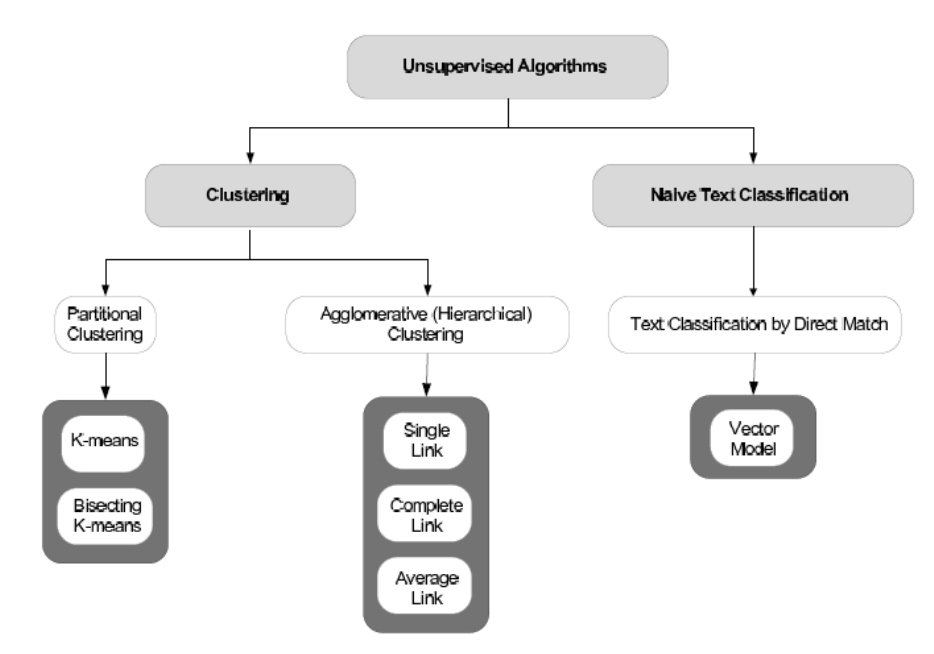
\includegraphics[scale=0.3]{assets/unsupervised-algo.png}
		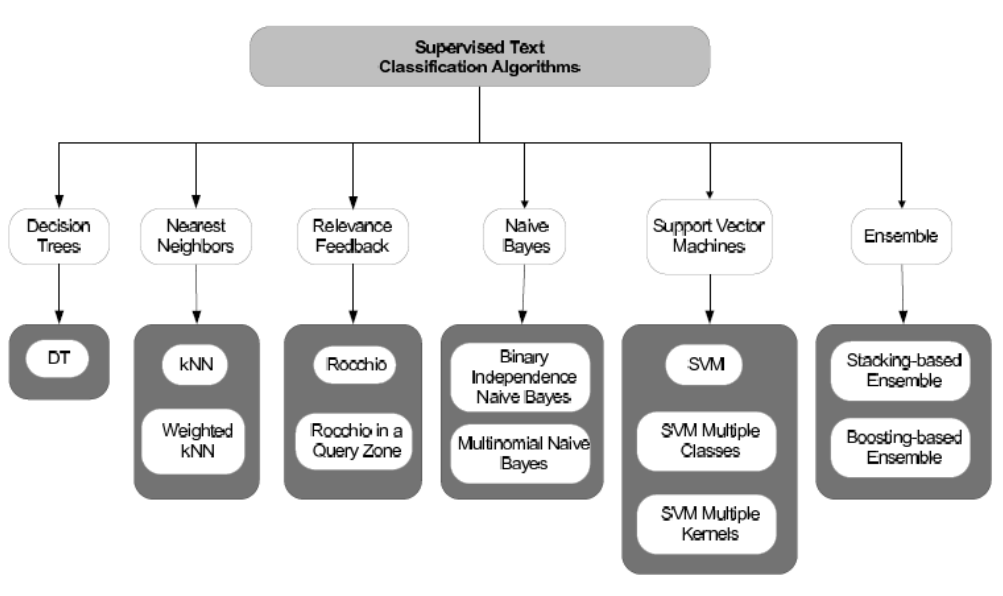
\includegraphics[scale=0.3]{assets/supervised-algo.png}
	\end{center}

	\subsection{Machine Learning per la Text Categorization}
	Possiamo definire il problema della text categorization come segue: data la descrizione di una istanza $x \in X$, dove $X$ è lo spazio delle istanze, e un insieme di classi $C = \{c_1, c_2, \ldots, c_L\}$, il problema consiste nel determinare la categoria di x, ovvero la classe $c \in C$ a cui appartiene: $x: c(x) \in C$ dove $c(x)$ è la funzione di classificazione il cui dominio è $X$ e il range è $C$.\\
	Un esempio di training è una istanza $x \in X$ associata alla categoria di appartenenza $c(x): <x, c(x)>$ dove c è una funzione di classificazione non nota. L'obiettivo del machine learning è quello di trovare una ipotesi di funzione di classificazione $h(x)$ tale che $\forall <x, c(x)> \in D: h(x) \approx c(x)$, dove $D$ è il training set. In questo caso si parla di consistenza dell'ipotesi.
	\vspace{\baselineskip}\\
	Ad esempio, consideriamo:
	\begin{itemize}
		\item lo spazio delle istanze <size, color, shape> dove:
		\begin{itemize}
			\item size = \{small, medium, large\}
			\item color = \{red, green, blue\}
			\item shape = \{circle, square, triangle\}
		\end{itemize}
		\item l'insieme delle classi C = \{positive, negative\}
		\item un training set D = 
		\begin{table}[H]
			\centering
			\begin{tabular}{|c|c|c|c|c|}
				\hline
				\textbf{Example} & \textbf{Size} & \textbf{Color} & \textbf{Shape} & \textbf{Class}\\ \hline
				1 & small & red & circle & positive\\ \hline
				2 & large & red & circle & negative\\ \hline
				3 & small & red & triangle & negative\\ \hline
				4 & large & blue & circle & negative\\ \hline
			\end{tabular}
		\end{table}
	\end{itemize} 
	L'obiettivo è quello di generalizzare le osservazioni al fine di classificare correttamente istanze future non presenti nel training set.\\
	Memorizzare semplicemente gli esempi garantisce la consistenza dell'ipotesi, ma non generalizza bene su nuovi esempi. Il processo di apprendimento mira a definire un modello generale di classificazioni che possa generalizzare su nuovi esempi.\\

	\section{Il problema della Text Categorization}
	La \textit{Text Categorization} è un problema di classificazione che consiste nel classificare automaticamente i documenti in base ai loro contenuti. L'obiettivo è quello di assegnare a ciascun documento una o più etichette che descrivano il tema o la categoria a cui appartiene. Questo processo è fondamentale per organizzare e gestire grandi collezioni di documenti, facilitando la ricerca e l'accesso alle informazioni.
	\vspace{\baselineskip}\\
	Formalmente, il problema della text categorization può essere definito come segue: dato un insieme di documenti $D$ e un insieme $C = \{c_1, c_2, \ldots, c_L\}$ di $L$ classi con le loro rispettive etichette, un classificatore di testo è una funzione binaria $\delta: D \times C \rightarrow \{0, 1\}$ che assegna un valore di verità a ciascuna coppia $(d_j, c_p)$, dove $d_j \in D$ è un documento e $c_p \in C$ è una classe, andando ad approssimare la funzione target $\delta': D \times C \rightarrow \{0,1\}$. Il valore di verità indica se il documento $d_j$ appartiene alla classe $c_p$ (1) o meno (0). Il classificatore di testo $\delta$ deve essere il più fedele possibile alla funzione target $\delta'$, in modo da generalizzare correttamente su nuovi documenti non presenti nel training set.
	\vspace{\baselineskip}\\
	Se nessuna restrizione è posta sul numero di classi assegnate a ciascun documento, il problema della text categorization è definito come un problema di classificazione \textbf{multi-label}. In questo caso, un documento può essere assegnato a più classi contemporaneamente, consentendo una maggiore flessibilità nella descrizione dei contenuti. Al contrario, se viene assegnata una sola etichetta a ciascun documento, il problema è definito come un problema di classificazione \textbf{single-label}. Il single-label è possibile solo nel caso vi sia indipendenza tra le classi, ovvero la presenza di una sola etichetta non influenza la presenza di altre etichette. Il caso del SL è più generale e usato molto più frequentemente rispetto al ML.

	\section{Train e Test}
	Sia $D = \{d_1, d_2, \ldots, d_{|D|}\}$ e $C = \{c_1, c_2, \ldots, c_{|C|}\}$, la funzione di classificazione $\delta'$ è nota per ogni valore di $<d_j, c_i> \in D \times C$. Se il suo valore è 1 allora si dice che $<d_j, c_i>$ è un esempio positivo per $\delta'$, altrimenti è un esempio negativo.\\  
	Definiamo due sotto-insiemi di $D$: il training set $Tr$ e il test set $Te$ tali che $Tr \cup Te = D$. Il classificatore è costruito a partire dalle osservazioni di Tr. Te è utilizzato per valutare le prestazioni del classificatore in fase di testing
	\vspace{\baselineskip}\\
	Algoritmi ad apprendimento supervisionato dipendono da un training set, costituito da un insieme di classi con esempi di documenti per ogni classe, il quale è utilizzato per addestrare il modello di classificazione. Più grande è il training set, maggiore è la capacità del modello di generalizzare su nuovi esempi. Si potrebbe però incorrere in un problema di \textit{overfitting}, ovvero il modello potrebbe adattarsi troppo ai dati di training, perdendo la capacità di generalizzare su nuovi esempi. 
	\begin{center}
		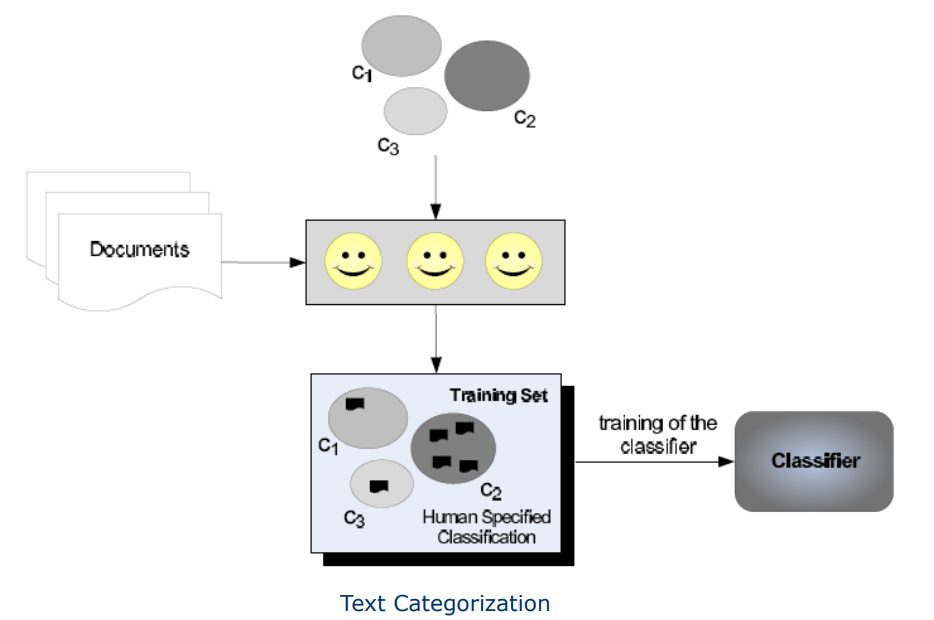
\includegraphics[scale=0.3]{assets/supervised-learning-training.png}
	\end{center}
	Per valutare il classificatore e misurare le sue prestazioni, è necessario utilizzare un test set separato, che contiene esempi non presenti nel training set. In questo modo è possibile effettuare una costruzione induttiva di un modello di classificazione che possa svolgere le funzioni di un sistema esperto, ovvero classificare correttamente nuovi documenti non presenti nel training set. 
	\begin{center}
		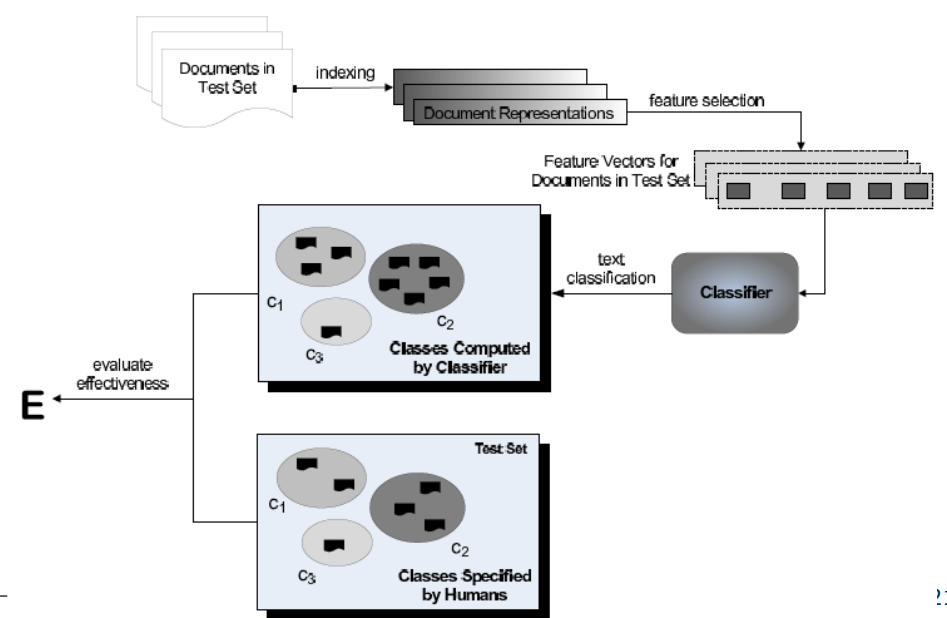
\includegraphics[scale=0.3]{assets/supervised-learning-testing.png}
	\end{center}
	In questo modo abbiamo una buona manutenibilità del sistema, in quanto non è necessario ingegnerizzare di continuo le regole di classificazione, ma è sufficiente aggiungere nuovi esempi al training set. D'altro canto , il modello necessita di una base di documenti pre-classificati che permettano di addestrarlo correttamente.

	\section{Indicizzazione}
	Prima di procedere con la classificazione dei documenti, è necessario effettuare una fase di \textit{indicizzazione}, ovvero la trasformazione dei documenti in un formato adatto per l'elaborazione automatica. Solitamente un documento $d_j$ viene rappresentato come un insieme di pesi, che indicano la presenza (o la frequenza) di termini tratti da un insieme di parole (o frasi). La scelta tipica per tale insieme è il \textbf{bag-of-words}, ovvero l'insieme di tutte le parole presenti nei documenti della collezione. Solitamente i pesi hanno valori in $[0,1]$ oppure assumono i soli valori 0 e 1 nel caso binario.
	\vspace{\baselineskip}\\
	Tipicamente, per calcolare i pesi dei termini, si utilizza la rappresentazione \textbf{TF-IDF} (\textit{Term Frequency-Inverse Document Frequency}). La \textit{Term Frequency} (TF) misura la frequenza di un termine in un documento, mentre la \textit{Inverse Document Frequency} (IDF) misura l'importanza di un termine rispetto all'intera collezione. Nello specifico, la TF-IDF è calcolata come segue:
	\[
		\text{TF-IDF}(t_k, d_j) = \#(t_k, d_j) \times \log\left(\frac{|Tr|}{\#_{Tr}(t_k)}\right)
	\]
	Per far ircadere i pesi in $[0,1]$, si può utilizzare la normalizzazione del coseno:
	\[
		w_{kj} = \frac{\text{TF-IDF}(t_k, d_j)}{\sqrt{\sum_{s=1}^{|T|} (TF-IDF(t_s, d_j))^2}}
	\]
	dove T è l'insieme dei termini che compaiono almeno una volta nei documenti di Tr. Prima dell'indicizzazione vengono rimosse le parole come articoli e proposizioni non relazionate con i topic in esame. L'uso dello stemming è controverso, in quanto può portare a una perdita di informazioni.

	\subsection{Riduzione della Dimensionalità}
	Un problema comune nella text categorization è la \textit{alta dimensionalità} dei dati, ovvero il numero elevato di termini che compongono i documenti. Questo può portare a problemi di \textit{overfitting} e a una riduzione delle prestazioni del classificatore. Per affrontare questo problema, è possibile utilizzare tecniche di \textit{riduzione della dimensionalità}, che consentono di proiettare i dati in uno spazio di dimensioni inferiori, mantenendo al contempo le informazioni rilevanti. Si può effettuare una riduzione locale della dimensionalità, ovvero ridurre la dimensionalità dei dati per ciascuna classe, oppure una riduzione globale, ovvero ridurre la dimensionalità dell'intero spazio dei dati e può essere effettuata per selezione o per estrazione. La selezione consiste nel selezionare un sottoinsieme di termini rilevanti, mentre l'estrazione consiste nel proiettare i dati in uno spazio di dimensioni inferiori.
	
	\subsubsection{Riduzione per Selezione}
	La riduzione per selezione consiste nel selezionare un sottoinsieme di termini rilevanti per la classificazione dei documenti. Questo può essere fatto utilizzando tecniche di \textit{feature selection}, che consentono di identificare i termini più informativi per ciascuna classe. Tra le tecniche più comuni vi sono:
	\begin{itemize}
		\item TSR - \textit{Term Space Reduction}: consiste nel selezionare un sotto insieme dell'insieme dei temrini che massimizzi l'efficienza al momento dell'indicizzazione;
		\item Wrapper: partendo da un insieme di termini, applica l'algortimo di learning a sotto insiemi di temrini ottenuti eliminando un termine alla volta fino a quando non si ottiene il miglior risultato;
		\item Filtering: seleziona  un sotto insieme di termini in accordo ai valori forniti da una funzione che misura l'importanza dei termini nel processo di categorizzazione.
	\end{itemize}

	\section{Relevance Feedback per la Text Categorization}
	Il \textit{Relevance Feedback} è una tecnica utilizzata per migliorare le prestazioni dei sistemi di categorizzazione del testo, consentendo agli utenti di fornire un feedback sulle classificazioni effettuate dal sistema. Questo feedback può essere utilizzato per aggiornare il modello di classificazione e migliorare la precisione delle previsioni. I documenti possono essere rappresentati usando un modello vettoriale, dove ciascun documento è rappresentato come un vettore di pesi associati ai termini presenti nel documento seguendo la rappresentazione TF-IDF normalizzato mediante la frequenza massima dei termini. Si assegnano documenti di testing alla categoria con il vettore prototipo più vicino secondo una misura di similarità.

	\subsection{Classificatore di Rocchio}
	Il classificatore di Rocchio è una tecnica di apprendimento supervisionato che si basa sul concetto di \textit{relevance feedback}, ovvero il feedback fornito dagli utenti sulle classificazioni effettuate dal sistema. L'obiettivo dell'algoritmo di Rocchio è quello di aggiornare il modello di classificazione in base al feedback fornito dagli utenti, migliorando così le prestazioni del sistema di categorizzazione del testo. 
	\vspace{\baselineskip}\\
	Se nel calcolo del relevance feedback, una query veniva modificata in base al feedback di rilevanza fornito dagli utenti, nel classificatore di Rocchio vengono interpretati i training set come se fossero informazioni di feedback. I termini che appartengono ad una specifica classe $c_p$ dei documenti di training sono considerati rilevanti quindi con feedback positivo, mentre i termini che non appartengono alla classe sono considerati non rilevanti quindi con feedback negativo. Le informazioni di feedback sono riassunte da un centroide a partire dal quale i nuovi documenti vengono classificati in base alla loro distanza dal centroide.
	\vspace{\baselineskip}\\
	Ogni documento $d_j$ è rappresentato come un vettore di termini pesato $\overrightarrow{d_j} = (w_{1j}, w_{2j}, \ldots, w_{tj})$, dove $w_{ij}$ è il peso del termine $k_i$ nel documento $d_j$ e $t$ è la dimensione del vocabolario. Il classificatore di Rocchio per una classe $c_p$ è calcolato come un centroide dato da:
	\[
		\overrightarrow{c_p} = \frac{\beta}{n_p} \sum_{d_j \in c_p} \overrightarrow{d_j} - \frac{\gamma}{N_t-n_p} \sum_{d_l \notin c_p} \overrightarrow{d_l}
	\]
	dove $n_p$ è il numero di documenti appartenenti alla classe $c_p$, $N_t$ è il numero di documenti nel training set, $\beta$ e $\gamma$ sono parametri che regolano l'importanza dei documenti appartenenti e non appartenenti alla classe $c_p$ rispettivamente.
	E' possibile utilizzare anche solamente i documenti appartenenti alla classe $c_p$ per calcolare il centroide.
	\vspace{\baselineskip}\\
	Nell'algoritmo di Rocchio, la classificazione è basata solamente sulla similarità dei documenti ai vettori prototipo delle classi, i quali non necessitano di medie o normalizzazioni poichè la similarità del coseno non è influenzata dalla lunghezza dei vettori. Utilizzando i vettori prototipo per ogni classe, l'algoritmo si riduce ad una semplice generalizzazione, senza garantire la consistenza dell'ipotesi.

	\section{Alberi di Decisione}
	Gli alberi di decisione sono una tecnica di apprendimento supervisionato utilizzata per la classificazione dei dati. Gli alberi di decisione sono costituiti da un insieme di nodi interni e foglie, dove ciascun nodo interno rappresenta un termine utilizzato per l'indicizzazione, le diramazioni dei nodi sono test sul peso dei termini nel documento di test e le foglie rappresentano le classi di appartenenza previste. La classificazione avviene testando ricorsivamente i valori dei pesi relativi ai termini associati ai nodi interni.
	\vspace{\baselineskip}\\
	Un metodo per il learning è invece il seguente:
	\begin{enumerate}
		\item verificare che tutti gli esempi di training appartengono alla stessa categoria ($c_i$ o la sua negazione);
		\item in caso negativo, selezionare un termine $t_k$ che partizioni il training set in classi di documenti in cui al termine $t_k$ è assegnato lo stesso valore, ponendo ciascuna classe in un sottoalbero diverso;
		\item ripetere ricorsivamente sui sotto-alberi finchè tutte le foglie non contengono esempi appartenenti alla stessa classe.
	\end{enumerate}
	La scelta di $t_k$ può essere effettuata massimizzando l'information gain.

	\section{Regole di Decisione}
	Le regole di decisione sono un'altra tecnica di apprendimento supervisionato utilizzata per la classificazione dei dati. Una regola di decisione per categorizzare un testo è espressa in forma normale disgiuntiva (disgiunzione di clausole congiuntive).
	\begin{table}[H]
		\centering
		\begin{tabular}{ccc}
			if & ((wheat \& farm) & or \\
			& (wheat \& commodity) & or \\
			& (bushels \& export) & or \\
			& (wheat \& tonnes) & or \\
			& (wheat \& winter \& $\neg$ soft)) & then wheat else $\neg$ wheat \\ 
		\end{tabular}
	\end{table}
	I classificatori basati su regole di decisione sono simili a quelli basati su alberi di decisione ma sono in genere più compatti. I letterali denotano la presenza o l'assenza di termini nel documento sotto esame, mentre la testa della clausola stabilisce di classificare sotto una data categoria. Inizialmente ogni esempio di training viene trasformato in una clausola congiuntiva $n_1, n_2, \ldots, n_M \rightarrow \gamma_i$ dove $n_i$ è un letterale e $\gamma_i$ è la classe di appartenenza e vale $c_i$ oppure la sua negazione. Un set di clausole è già un classificatore che però causa overfitting. Attraverso una procedura di generalizzazione il set viene sempligicato il più possibile giungendo ad una rappresentazione compatta che non sacrifichi la precisione.
	
	\section{Nearest-Neighbor Learning Algorithm}
	Il \textbf{Nearest Neighbor Learning Algorithm} è un approccio di apprendimento supervisionato che si basa sul confronto diretto tra istanze. A differenza di molti altri algoritmi di machine learning, non costruisce un modello esplicito o una generalizzazione dei dati di training. Invece, si limita a memorizzare gli esempi presenti nel training set, denotato come \(Tr\), e utilizza questi esempi per effettuare previsioni.
	\vspace{\baselineskip}\\
	Quando viene fornita una nuova istanza di test, indicata con \(x\), l'algoritmo calcola la similarità tra questa istanza e tutti gli esempi presenti nel training set. Una volta identificate le similarità, assegna a \(x\) la classe associata all'esempio più simile in \(Tr\). Questo approccio si distingue per la sua semplicità, poiché non effettua alcuna generalizzazione o sintesi dei dati, né crea prototipi per rappresentare le categorie. In altre parole, il \textit{training set} stesso funge da classificatore.
	\vspace{\baselineskip}\\
	Questa caratteristica lo rende computazionalmente costoso, soprattutto in contesti con grandi quantità di dati, perché per ogni istanza di test è necessario calcolare la similarità con tutti gli esempi di \(Tr\). Inoltre, il \textit{Nearest Neighbor Learning Algorithm} appartiene a una classe di metodi nota come \textit{case-based learning}, in cui ogni decisione è basata su esempi specifici del training set. È anche classificato come \textit{memory-based learning}, in quanto richiede di memorizzare l'intero dataset di training. Infine, è considerato un metodo di \textit{lazy learning}, poiché non prevede una fase esplicita di addestramento: l'algoritmo lavora direttamente sui dati al momento della previsione.

	\section{K-Nearest Neighbor (k-NN)}
	Il \textit{Nearest Neighbor Learning Algorithm} presenta alcuni limiti significativi, in particolare la sua sensibilità agli esempi atipici, noti come \textit{outlier}, e agli errori nelle etichette degli esempi nel training set. Per superare queste problematiche, è stato sviluppato un approccio migliorato chiamato \textbf{k-Nearest Neighbor}, abbreviato in \textit{k-NN}. Questo metodo non si basa esclusivamente sull'esempio più vicino, ma considera i \(k\) esempi più simili all'istanza di test e assegna a quest'ultima la classe che risulta essere più frequente tra questi \(k\) esempi.
	\vspace{\baselineskip}\\
	L'idea di considerare più vicini consente di ridurre l'impatto di eventuali \textit{outlier}, che potrebbero influenzare negativamente il risultato della classificazione. Inoltre, questo approccio è meno sensibile al rumore presente nei dati, in particolare agli errori nelle etichette. La scelta del parametro \(k\) è un aspetto cruciale per il corretto funzionamento dell'algoritmo. Valori troppo piccoli di \(k\) possono rendere il modello sensibile agli \textit{outlier}, mentre valori troppo grandi possono diluire l'informazione locale. Per evitare situazioni di parità tra le classi, si sceglie comunemente un valore dispari per \(k\). I valori più utilizzati sono 3 e 5, poiché rappresentano un buon compromesso tra robustezza e accuratezza.
	\vspace{\baselineskip}\\
	Sia il \textit{Nearest Neighbor Learning Algorithm} sia il \textit{k-NN} si basano su una misura di similarità, o distanza, per confrontare le istanze. La scelta della metrica di similarità è un elemento determinante per il successo dell'algoritmo e dipende strettamente dalla natura dei dati su cui si opera. Nel caso di dati testuali, una delle metriche più efficaci è la \textit{similarità del coseno}, calcolata tra vettori rappresentati attraverso il \textit{TF-IDF}. La \textit{similarità del coseno} si è dimostrata particolarmente adatta per catturare la somiglianza relativa tra documenti, poiché non tiene conto della lunghezza assoluta dei vettori, ma si concentra sulla loro direzione nello spazio. Questa proprietà la rende efficace per classificare documenti testuali basandosi sulle relazioni semantiche tra i termini.
	\vspace{\baselineskip}\\
	Nella fase di Training, per ogni esempio $<x, c(x)> \in Tr$, dove $x$ è un documento e $c(x)$ è la classe di appartenenza, si calcola il vettore di pesi TF-IDF normalizzato $d_x$ per il documento $x$. Durante la fase di Testing, si calcola il vettore di pesi TF-IDF normalizzato $d$ per il documento y da classificare. Per ogni esempio $<x, c(x)> \in Tr$, si calcola la similarità del coseno tra $d$ e $d_x$. Si ordinano gli esempi in base alla similarità del coseno e si selezionano i $k$ esempi più simili. Infine, si assegna a $y$ la classe più frequente tra i $k$ esempi selezionati.

	\section{Cenni di Probabilità}
	Gli \textbf{assiomi della teoria della probabilità} forniscono la base matematica per calcolare le probabilità in modo rigoroso e coerente.

	\begin{itemize}
    	\item \textbf{Intervallo di probabilità:}  
    	Qualsiasi probabilità $P(A)$ deve essere compresa tra 0 e 1:
		\[
		0 \leq P(A) \leq 1
		\]
		\item \textbf{Valori estremi:}  
		\[
		P(\text{true}) = 1, \quad P(\text{false}) = 0
		\]
		\item \textbf{Disgiunzione di eventi:}  
		La probabilità che accada almeno uno tra due eventi $A$ e $B$ (cioè $P(A \lor B)$) si calcola come:
		\[
		P(A \lor B) = P(A) + P(B) - P(A \land B)
		\]
	\end{itemize}
	La \textbf{probabilità condizionata} esprime la probabilità che un evento $A$ accada dato che un altro evento $B$ è già noto. Si indica con $P(A \mid B)$ ed è definita dalla formula:
	\[
	P(A \mid B) = \frac{P(A \land B)}{P(B)}
	\]
	L'\textbf{indipendenza} tra due eventi $A$ e $B$ si verifica quando la probabilità che accada $A$ non è influenzata dalla conoscenza dell'evento $B$. In questo caso, la probabilità condizionata $P(A \mid B)$ è uguale alla probabilità marginale $P(A)$:
	\[
	P(A \mid B) = P(A)
	\]
	Questo perchè, sapendo che $P(A \land B) = P(A) \cdot P(B)$, si ha:
	\[
	P(A \mid B) = \frac{P(A \land B)}{P(B)} = \frac{P(A) \cdot P(B)}{P(B)} = P(A)
	\]

	\section{Metodo Bayesiano}
	I metodi bayesiani sono tecniche di apprendimento e classificazione basate sulla teoria della probabilità. Questi metodi sfruttano il \textbf{teorema di Bayes}, che rappresenta una componente essenziale per apprendere e classificare in modo probabilistico.
	\begin{itemize}
		\item \textbf{Probabilità a priori (prior):}  
		La probabilità a priori rappresenta la probabilità di ogni categoria prima di avere nuove informazioni. È ciò che sappiamo inizialmente senza dati aggiuntivi.
		\item \textbf{Probabilità a posteriori (posterior):}  
		Dopo aver osservato un elemento o una descrizione, il modello produce una probabilità aggiornata, chiamata probabilità a posteriori, che indica la distribuzione delle probabilità tra le possibili categorie di appartenenza.
	\end{itemize}
	L'obiettivo è assegnare un elemento alla categoria più probabile, utilizzando queste distribuzioni. Ad esempio, dato un documento di testo, si stima la probabilità che appartenga a una specifica categoria (come notizie sportive, economiche, ecc.), calcolando il risultato basato sui dati di training.
	\vspace{\baselineskip}\\
	Il \textbf{teorema di Bayes} è una formula che consente di calcolare la probabilità a posteriori di un'ipotesi, data l'evidenza. La formula è la seguente:
	\[
	P(H \mid E) = \frac{P(E \mid H) \cdot P(H)}{P(E)}
	\]
	dove $P(H \mid E)$ è la probabilità a posteriori dell'ipotesi $H$ data l'evidenza $E$, $P(E \mid H)$ è la probabilità dell'evidenza $E$ data l'ipotesi $H$, $P(H)$ è la probabilità a priori dell'ipotesi $H$ e $P(E)$ è la probabilità dell'evidenza $E$.
	\vspace{\baselineskip}\\
	Nel contesto della classificazione del testo, l'obiettivo è assegnare un documento $d$ alla classe $c$ che massimizza la probabilità a posteriori $P(c \mid d)$. Questa probabilità può essere calcolata utilizzando il teorema di Bayes come segue:
	\[
	P(c_i \mid d) = \frac{P(d \mid c_i) \cdot P(c_i)}{P(d)}
	\]
	Per definire la classe $c_i$ che massimizza la probabilità a posteriori $P(c_i \mid d)$, e che quindi è assegnata al documento $d$, si calcola la probabilità a posteriori per ogni classe e si seleziona quella con il valore massimo:
	\[
	c = \text{argmax}_{c_i} P(c_i \mid d)
	\]
	Considerando che $P(d)$ è costante per tutte le classi, è possibile semplificare la formula come segue:
	\[
	c = \text{argmax}_{c_i} P(c_i \mid d) = \text{argmax}_{c_i} P(d \mid c_i) \cdot P(c_i)
	\]
	Per calcolare la probabilità $P(d \mid c_i)$, si utilizza il modello di classificazione, ad esempio un classificatore bayesiano, che stima la probabilità di un documento $d$ dato che appartiene alla classe $c_i$. La probabilità $P(c_i)$ è la probabilità a priori della classe $c_i$, che può essere calcolata a partire dai dati di training: $P(c_i) = \frac{n_i}{N}$, dove $n_i$ è il numero di documenti del training set appartenenti alla classe $c_i$ e $N$ è il numero totale di documenti nel training set.
	Adesso si può calcolare la probabilità a posteriori $P(d \mid c_i)$ per ogni classe $c_i$: $P(d \mid c_i) = P(t_1 \land t_2 \land \ldots \land t_n \mid c_i)$, dove $t_1, t_2, \ldots, t_n$ sono i termini presenti nel documento $d$. Questo sarebbe molto costoso da calcolare, quindi si utilizza l'assunzione di indipendenza condizionale, nonostante sia inverosimile che i termini siano indipendenti tra loro. Questa assunzione semplifica il calcolo della probabilità a posteriori come segue:
	\[
	P(d \mid c_i) = P(t_1 \mid c_i) \cdot P(t_2 \mid c_i) \cdot \ldots \cdot P(t_n \mid c_i) = \prod_{j=1}^{k} P(t_j \mid c_i)
	\] 
	dove  $P(t_j \mid c_i)$ è la probabilità che il termine $t_j$ appaia in un documento della classe $c_i$:
	\[
	P(t_j \mid c_i) = \frac{N_{t_j, c_i}}{N_{c_i}}
	\]
	dove $N_{t_j, c_i}$ è il numero di volte che il termine $t_j$ appare nei documenti della classe $c_i$ e $N_{c_i}$ è il numero totale di termini nei documenti della classe $c_i$. E' presente, però, un problema per quanto riguarda il precedente calcolo, ovvero la presenza di termini che non compaiono nei documenti di una classe e che porterebbero a probabilità nulle azzerando il prodotto. Per risolvere questo problema si utilizza la tecnica della \textbf{smoothing di Laplace - Categorizzazione Bayesiana Naive}, che consiste nel far si che la probabilità di un termine sia maggiore di 0 anche se non compare nei documenti di una classe. Di conseguenza i termini non presenti nei documenti di una classe avranno una occorrenza minima, ma non nulla. Gli altri termini, invece, avranno una probabilità superiore a quella dei termini non presenti. La probabilità di un termine $t_j$ dato che appartiene alla classe $c_i$ diventa:
	\[
	P(t_j \mid c_i) = \frac{N_{t_j, c_i} + 1}{N_{c_i} + |V|}
	\]
	dove $|V|$ è la dimensione del vocabolario, ovvero il numero totale di termini presenti nei documenti di training.

	\begin{tcolorbox}[title=Esercizio di esempio]
		Si consideri un problema di classificazione del testo con due classi $C = \{c_1, c_2\}$ e una collezione di 500 documenti su un vocabolario $V = {t_1, t_2, t_3, t_4}$. Costruire il classificatore bayesiano sul training set seguente:
		\[
			\{<d_1, c_1>, <d_2, c_1>, <d_3, c_1>, <d_4, c_2>\}
		\]
		dove ogni documento è rappresentato dalla bag-of-words:
		\[
			\begin{array}{l}
				d_1 = \{t_1: 1, t_4: 2\} \quad
				d_2 = \{t_3: 2, t_1: 3\} \quad
				d_3 = \{t_1: 3, t_3: 4\} \\
				d_4 = \{t_1: 6, t_4: 7\}
			\end{array}
		\]
		\textbf{Soluzione:}\\
			Il classificatore di Bayes calcola la probabilità a posteriori $P(c_i \mid d)$ per ogni classe $c_i$ e assegna il documento $d$ alla classe con la probabilità più alta. Per calcolare la probabilità a posteriori, si utilizza il teorema di Bayes:
			\[
				P(c_i \mid d) = \frac{P(d \mid c_i) \cdot P(c_i)}{P(d)}
			\]
			Posso omettere $P(d)$ in quanto è costante per tutte le classi.
			\vspace{\baselineskip}\\
			Per prima cosa calcolo le probabilità a priori $P(c_i)$ per le classi $c_1$ e $c_2$:
			\[
				\begin{array}{l}
					P(c_i) = \frac{n_i}{N} \\
					P(c_1) = \frac{3}{4} = 0.75 \quad P(c_2) = \frac{1}{4} = 0.25
				\end{array}
			\]
			dove $n_i$ è il numero di documenti della classe $c_i$ e $N$ è il numero totale di documenti nel training set.
			\vspace{\baselineskip}\\
			Successivamente calcolo la probabilità $P(d \mid c_i)$ per ogni classe $c_i$:
			\[
				\begin{array}{l}
					P(d \mid c_i) = P(t_1 \land \dots \land t_k \mid c_i) \\
					\text{assumo che i termini siano indipendenti} \\
					P(d \mid c_i) = P(t_1 \mid c_i) \cdot P(t_2 \mid c_i) \cdot \dots \cdot P(t_k \mid c_i) = \prod_{j=1}^{k} P(t_j \mid c_i) \\
					P(t_j \mid c_i) = \frac{N_{t_j, c_i} + 1}{N_{c_i} + |V|} \\\\
					\begin{array}{l}
						P(t_1 \mid c_1) = \frac{1+3+3+1}{15+4} = \frac{8}{19} \\
						P(t_2 \mid c_1) = \frac{0+1}{15+4} = \frac{1}{19} \\
						P(t_3 \mid c_1) = \frac{2+4+1}{15+4} = \frac{7}{19} \\
						P(t_4 \mid c_1) = \frac{2+1}{15+4} = \frac{3}{19} \\\\
						P(t_1 \mid c_2) = \frac{6+1}{13+4} = \frac{7}{17} \\
						P(t_2 \mid c_2) = \frac{0+1}{13+4} = \frac{1}{17} \\
						P(t_3 \mid c_2) = \frac{0+1}{13+4} = \frac{1}{17} \\
						P(t_4 \mid c_2) = \frac{7+1}{13+4} = \frac{8}{17}
					\end{array}
				\end{array}
			\]
			Andiamo a classificare il documento $d: \{t_1: 1, t_2:3\}$:
			Per la classe $c_1$:
			\[
				\begin{array}{l}
					\alpha = P(c_1 \mid d) = P(c_1) \cdot P(d \mid c_1) = \frac{3}{4} \cdot P(t_1 \land t_2 \land t_2 \land t_2 \mid c_1)\\
					\text{per l'assunzione di indipendenza} \\
					\alpha = P(c_1 \mid d) = \frac{3}{4} \cdot P(t_1 \mid c_1) \cdot P(t_2 \mid c_1) \cdot P(t_2 \mid c_1) \cdot P(t_2 \mid c_1) = \\ = \frac{3}{4} \cdot P(t_1 \mid c_1)^1 \cdot P(t_2 \mid c_1)^3 = \frac{3}{4} \cdot \left(\frac{8}{19}\right) \cdot \left(\frac{1}{19}\right)^3 = \frac{3}{4} \cdot \frac{8}{19} \cdot \frac{1}{6859} = \frac{24}{5146} \approx 0.0047
				\end{array}
			\]
			Per la classe $c_2$:
			\[
				\begin{array}{l}
					\beta = P(c_2 \mid d) = P(c_2) \cdot P(d \mid c_2) = \frac{1}{4} \cdot P(t_1 \land t_2 \land t_2 \land t_2 \mid c_2)\\
					\text{per l'assunzione di indipendenza} \\
					\beta = P(c_2 \mid d) = \frac{1}{4} \cdot P(t_1 \mid c_2) \cdot P(t_2 \mid c_2) \cdot P(t_2 \mid c_2) \cdot P(t_2 \mid c_2) =\\= \frac{1}{4} \cdot P(t_1 \mid c_2)^1 \cdot P(t_2 \mid c_2)^3 = \frac{1}{4} \cdot \left(\frac{7}{17}\right) \cdot \left(\frac{1}{17}\right)^3 = \frac{1}{4} \cdot \frac{7}{17} \cdot \frac{1}{4913} = \frac{7}{69652} \approx 0.0001
				\end{array}
			\]
			La probabilità a posteriori $\alpha$ per la classe $c_1$ è maggiore rispetto a $\beta$ per la classe $c_2$, quindi il documento $d$ viene classificato come appartenente alla classe $c_1$.
	\end{tcolorbox}

	\subsection{Prevenzione dell'underflow}
	Quando si lavora con probabilità molto piccole, nell'intervallo $[0,1]$, si può incorrere in problemi di \textit{underflow}, ovvero la perdita di precisione a causa della rappresentazione numerica. Per evitare questo problema, si può utilizzare il logaritmo delle probabilità, trasformando il prodotto in somma:
	\[
		\log(a \cdot b) = \log(a) + \log(b)
	\]
	Di conseguenza, la classe con il valore massimo del logaritmo delle probabilità a posteriori è quella assegnata al documento.
	\vspace{\baselineskip}\\
	I risultati della classificazione bayesiana naive sono tendenzialmente molto accurati. Nonostante ciò, a causa dell'assunzione di indipendenza condizionale tra i termini, la stima numerica della probabilità a posteriori effettiva non è sempre accurata.

	\section{Valutazione di un Classificatore}
	La valutazione di un classificatore è un aspetto fondamentale per misurarne l'efficacia e l'accuratezza. Essa è sperimentale poichè il problema non ha una specifica formale che consenta un altro tipo di valutazione. La valutazione deve essere effettuata su dati di test indipendenti dai dati di training, in modo da ottenere una stima realistica delle prestazioni del classificatore. La \textbf{classification accuracy} è una misura comune per valutare la bontà di un classificatore. Essa rappresenta la percentuale di documenti classificati correttamente rispetto al totale dei documenti di test. La classification accuracy si calcola come segue:
	\[
		\text{Classification Accuracy} = \frac{\text{Numero di istanze di testing classificate correttamente}}{\text{Numero totale di istanze di testing}}
	\]
	I risultati possono variare in base alla scelta del training set e del test set. Solitamente si mediano i risultati ottenuti su più training e test set per ottenere una stima più accurata delle prestazioni del classificatore.
	\vspace{\baselineskip}\\
	Le misure standard per valutare l'efficacia di un classificatore sono \textbf{precision} ($\pi$) e \textbf{recall} ($\rho$), termini mutuati dall'Information Retrieval (IR). La \textit{precision}, indicata con $\pi$, può essere interpretata come una misura di \textit{correttezza}, che indica la proporzione di elementi classificati correttamente come positivi rispetto a tutti gli elementi classificati come positivi. La \textit{recall}, indicata con $\rho$, rappresenta invece la \textit{completezza}, ovvero la proporzione di elementi positivi correttamente individuati rispetto a tutti gli elementi realmente positivi.
	\vspace{\baselineskip}\\
	Sia $C = \{c_1, c_2, \dots, c_{|C|}\}$ l'insieme delle categorie, e per ogni categoria $c_i$ definiamo:
	\begin{align*}
		\hat{\pi}_i &= \frac{TP_i}{TP_i + FP_i}, \\
		\hat{\rho}_i &= \frac{TP_i}{TP_i + FN_i}.
	\end{align*}
	dove:
	\begin{itemize}
		\item $TP_i$ (\textit{True Positives}) indica il numero di elementi correttamente classificati come appartenenti alla categoria $c_i$.
		\item $FP_i$ (\textit{False Positives}) è il numero di elementi erroneamente classificati come appartenenti alla categoria $c_i$.
		\item $FN_i$ (\textit{False Negatives}) rappresenta il numero di elementi appartenenti alla categoria $c_i$ ma classificati erroneamente come non appartenenti.
		\item $TN_i$ (\textit{True Negatives}) indica il numero di elementi correttamente classificati come non appartenenti alla categoria $c_i$.
	\end{itemize}
	Per valutare un classificatore su più categorie, è possibile utilizzare due approcci di aggregazione: \textbf{microaveraging} e \textbf{macroaveraging}. Il microaveraging considera il contributo di ogni categoria proporzionalmente al numero di elementi. Le formule per precision e recall in questo approccio sono:
	\begin{align*}
		\hat{\pi}_{\text{micro}} &= \frac{\sum_{i=1}^{|C|} TP_i}{\sum_{i=1}^{|C|} TP_i + \sum_{i=1}^{|C|} FP_i}, \\
		\hat{\rho}_{\text{micro}} &= \frac{\sum_{i=1}^{|C|} TP_i}{\sum_{i=1}^{|C|} TP_i + \sum_{i=1}^{|C|} FN_i}.
	\end{align*}
	Il macroaveraging assegna uguale peso a ciascuna categoria, indipendentemente dal numero di elementi, calcolando la media aritmetica delle misure individuali:
	\begin{align*}
		\hat{\pi}_{\text{macro}} &= \frac{1}{|C|} \sum_{i=1}^{|C|} \hat{\pi}_i, \\
		\hat{\rho}_{\text{macro}} &= \frac{1}{|C|} \sum_{i=1}^{|C|} \hat{\rho}_i.
	\end{align*}
	La scelta tra microaveraging e macroaveraging dipende dal contesto applicativo. Il microaveraging è preferito quando l'interesse principale è bilanciare gli errori su tutti gli elementi, mentre il macroaveraging è utile per dare uguale importanza alle diverse categorie, anche se sbilanciate in termini di numerosità.

	\section{K-Fold Cross-Validation}
	La \textbf{K-Fold Cross-Validation} è una tecnica di valutazione che permette di ottenere una stima più accurata delle prestazioni di un classificatore. Considerando che i risultati possono variare in base alla scelta del training set e del test set, la K-Fold Cross-Validation suddivide il dataset in $K$ insiemi disgiunti, chiamati \textit{fold}, e per ogni fold esegue una fase di test addestrando il sistema sui restanti $K-1$ fold. Questo processo viene ripetuto $K$ volte, in modo che ciascun fold venga utilizzato una volta come test set. Infine, si calcolano le medie delle misure di valutazione ottenute su ciascun fold. Tipicamente si utilizza la K-Fold Cross-Validation con $K=10$, ma il valore di $K$ può variare a seconda del dataset e del problema specifico. La procedura garantisce l'indipendenza tra training e test set, riducendo il rischio di overfitting e fornendo una stima più accurata delle prestazioni del classificatore.

	\section{Curve di Learning}
	Nei contesti applicativi reali, ottenere dataset già etichettati non è sempre semplice. Inoltre, la quantità di dati disponibili può variare notevolmente da un problema all'altro. Osservare il variare dell'accuratezza predittiva di un classificatore in base al numero di istanze usate nella fase di learning è un aspetto importante per comprendere il comportamento del modello. Le \textbf{curve di apprendimento} rappresentano graficamente l'andamento dell'accuratezza del classificatore in funzione dei dati di test indipendenti (asse Y) rispetto al numero di istanze di training (asse X). Esse possono essere mediate sulle varie prove indipendenti del K-Fold Cross-Validation per ottenere una stima più accurata delle prestazioni del classificatore per ogni prova e per ogni numero di istanze di training, andando a misurare la variazione dell'accuratezza in funzione della quantità di dati disponibili per ogni punto della curva.
	\begin{center}
		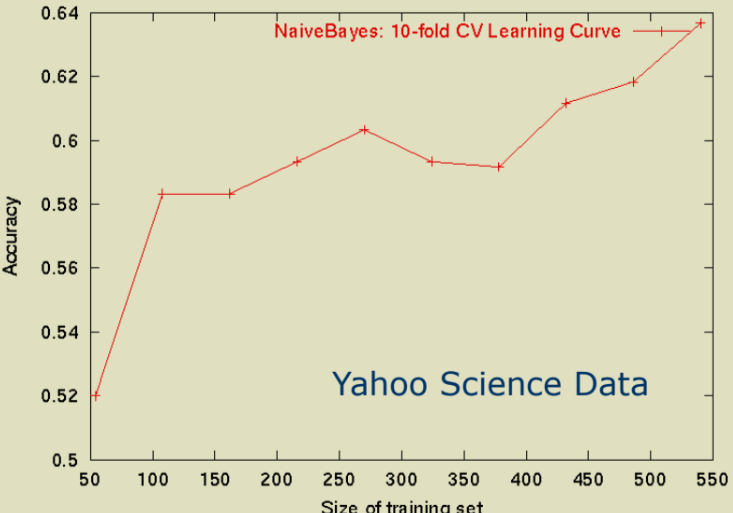
\includegraphics[scale=0.5]{assets/learning-curve.png}
	\end{center}

	\chapter{Page Rank}
	\section{Introduzione}
	Il \textbf{Page Rank} è un algoritmo di classificazione delle pagine web sviluppato da Larry Page e Sergey Brin, fondatori di Google. L'obiettivo principale di Page Rank è assegnare un punteggio numerico a ciascuna pagina web, in modo da determinare la sua rilevanza e importanza all'interno del web. Il punteggio di Page Rank è calcolato in base alla struttura del grafo delle pagine web, considerando i collegamenti ipertestuali tra le pagine stesse. L'idea alla base di Page Rank è che una pagina web è più importante se è collegata da altre pagine importanti. In altre parole, il punteggio di Page Rank di una pagina è influenzato dalla quantità e dalla qualità dei link in ingresso.

	\section{Links come voti}
	La struttura del web può essere rappresentata come un grafo diretto, in cui i nodi corrispondono alle pagine web e gli archi rappresentano i collegamenti ipertestuali tra le pagine. Ogni collegamento da una pagina $A$ a una pagina $B$ può essere interpretato come un voto di $A$ a favore di $B$. In questo contesto, il Page Rank di una pagina web $A$ è calcolato in base ai voti ricevuti da altre pagine web. L'importanza di una pagina è determinata dalla quantità e dalla qualità dei voti ricevuti. In particolare, un voto da una pagina web con un alto Page Rank ha un peso maggiore rispetto a un voto da una pagina con un Page Rank basso.
	\begin{center}
		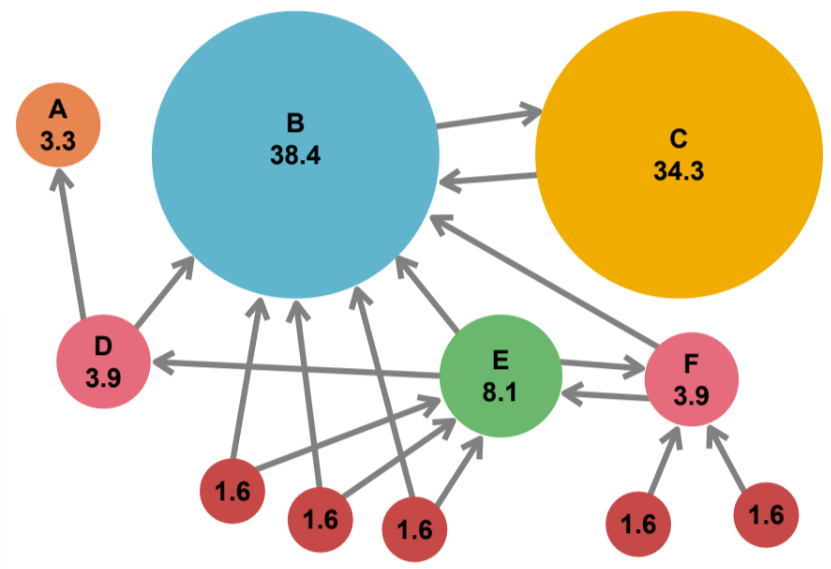
\includegraphics[scale=0.5]{assets/page-rank-graph.png}
	\end{center}
	Ogni voto di un arco è proporzionale al Page Rank della pagina sorgente. Se la pagina j con importanza $r_j$ ha $n_j$ link uscenti, allora ogni link trasmette un voto di importanza $r_j/n_j$ alla pagina di destinazione. L'importanza di una pagina è la somma dei voti ricevuti da tutte le pagine che puntano ad essa.
	\begin{center}
		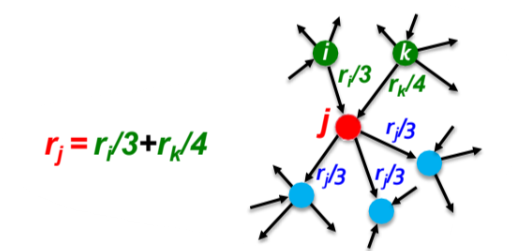
\includegraphics[scale=0.5]{assets/page-rank-votes.png}
	\end{center}
	Una pagina è ritenuta importante se è destinataria di link uscenti da altre pagine importanti. Il rank di una pagina j si definisce come:
	\[
		r_j = \sum_{i \rightarrow j} \frac{r_i}{d_i}
	\]
	dove $i \rightarrow j$ indica che la pagina i punta alla pagina j, $r_i$ è il rank della pagina i, $d_i$ è il numero di link uscenti dalla pagina i.

	\section{Formulazione Matriciale}
	Il problema del calcolo del \textit{PageRank} può essere inizialmente modellato attraverso un sistema di equazioni di flusso che descrivono la distribuzione delle "rilevanze" tra tre nodi (\texttt{y}, \texttt{a}, \texttt{m}). Le equazioni che regolano i flussi sono:
	\[
	r_y = \frac{r_y}{2} + \frac{r_a}{2}, \quad
	r_a = \frac{r_y}{2} + r_m, \quad
	r_m = \frac{r_a}{2}.
	\]
	Tuttavia, queste tre equazioni con tre incognite non includono costanti, rendendo impossibile ottenere una soluzione unica. In effetti, tutte le soluzioni sono equivalenti modulo un fattore di scala.

	Per risolvere questa indeterminatezza, si aggiunge un ulteriore vincolo:
	\[
	r_y + r_a + r_m = 1.
	\]
	Con questa condizione, la soluzione diventa unica e si ottiene:
	\[
	r_y = \frac{2}{5}, \quad r_a = \frac{2}{5}, \quad r_m = \frac{1}{5}.
	\]
	Anche se il metodo di eliminazione gaussiana funziona bene per piccoli esempi come questo, risulta inefficiente per grafi di grandi dimensioni, come quelli del web. È quindi necessario adottare una nuova formulazione.

	La soluzione matriciale si basa sull'uso della matrice di adiacenza stocastica, denotata con $M$. Per costruirla, si considerano i seguenti principi:
	\begin{itemize}
		\item Se una pagina $i$ ha $d_i$ collegamenti in uscita, allora il peso di ogni collegamento verso una pagina $j$ è dato da $M_{ji} = \frac{1}{d_i}$.
		\item Se non c'è collegamento tra $i$ e $j$, si ha $M_{ji} = 0$.
	\end{itemize}
	La matrice $M$ è una \textit{matrice stocastica colonna}, ovvero ogni colonna della matrice somma a 1. Questo approccio matriciale permette di calcolare il \textit{PageRank} in modo scalabile, anche per grafi di grandi dimensioni.

	\begin{center}
		\begin{tabular}{ccc}
			% Grafo
			\begin{tikzpicture}
				% Nodes
				\node[circle, draw, fill=red!70, text=white] (y) at (0, 1.5) {\textbf{y}};
				\node[circle, draw, fill=red!70, text=white] (a) at (2, 0) {\textbf{a}};
				\node[circle, draw, fill=red!70, text=white] (m) at (4, 0) {\textbf{m}};
	
				% Arrows
				\draw[->, thick] (y) edge[bend left=20] (a);
				\draw[->, thick] (a) edge[bend left=20] (y);
				\draw[->, thick] (a) edge (m);
				\draw[->, thick] (m) edge[bend left=20] (a);
				\draw[->, thick] (y) edge[loop above] (y);
			\end{tikzpicture}
			&
			% Tabella
			\(\begin{array}{c|ccc}
				& \mathbf{y} & \mathbf{a} & \mathbf{m} \\ \hline
				\mathbf{y} & \frac{1}{2} & \frac{1}{2} & 0 \\
				\mathbf{a} & \frac{1}{2} & 0 & 1 \\
				\mathbf{m} & 0 & \frac{1}{2} & 0 \\
			\end{array}\)
			&
			% Equazioni
			\(\begin{aligned}
				r_y &= \frac{r_y}{2} + \frac{r_a}{2} \\
				r_a &= \frac{r_y}{2} + r_m \\
				r_m &= \frac{r_a}{2}
			\end{aligned}\)
		\end{tabular}
	\end{center}
	Dato un vettore di rank $r$, che contiene una entry per ogni pagina web, con $r_i$ che rappresenta lo score di Page Rank della pagina $i$, l'equazione di flusso può essere riscritta in forma matriciale come:
	\[
	r = M \cdot r.
	\]
	Supponiamo che la pagina $i$ abbia un link con 3 pagine, inclusa $j$.
	\begin{center}
		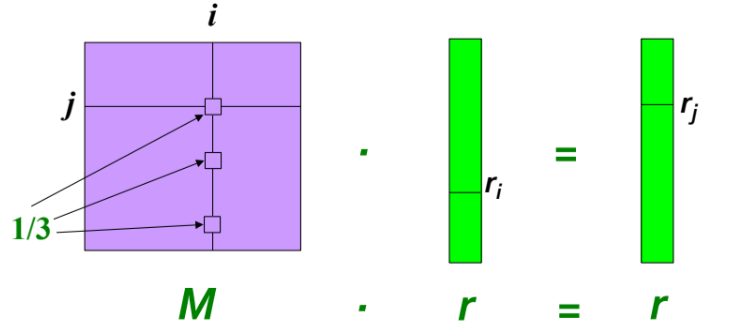
\includegraphics[scale=0.4]{assets/page-rank-matrix-ex.png}
	\end{center}
	In questo modo, il vettore di rank $r$ è un autovettore della matrice stocastica $M$. Infatti, al primo o il principale autovettore della matrice $M$ corrisponde l'autovalore 1. Il massimo autovalore di M è 1 poichè M è una matrice stocastica su colonne.

	\begin{center}
		\begin{tabular}{cccc}
			% Grafo
			\begin{tikzpicture}
				% Nodes
				\node[circle, draw, fill=red!70, text=white] (y) at (0, 1.5) {\textbf{y}};
				\node[circle, draw, fill=red!70, text=white] (a) at (2, 0) {\textbf{a}};
				\node[circle, draw, fill=red!70, text=white] (m) at (4, 0) {\textbf{m}};
	
				% Arrows
				\draw[->, thick] (y) edge[bend left=20] (a);
				\draw[->, thick] (a) edge[bend left=20] (y);
				\draw[->, thick] (a) edge (m);
				\draw[->, thick] (m) edge[bend left=20] (a);
				\draw[->, thick] (y) edge[loop above] (y);
			\end{tikzpicture}
			&
			% Tabella
			\(\begin{array}{c|ccc}
				& \mathbf{y} & \mathbf{a} & \mathbf{m} \\ \hline
				\mathbf{y} & \frac{1}{2} & \frac{1}{2} & 0 \\
				\mathbf{a} & \frac{1}{2} & 0 & 1 \\
				\mathbf{m} & 0 & \frac{1}{2} & 0 \\
			\end{array}\)
			&
			% Equazioni
			\(\begin{aligned}
				r_y &= \frac{r_y}{2} + \frac{r_a}{2} \\
				r_a &= \frac{r_y}{2} + r_m \\
				r_m &= \frac{r_a}{2}
			\end{aligned}\)
			&
			\(
			\begin{bmatrix}
			y \\ a \\ m
			\end{bmatrix}
			=
			\begin{bmatrix}
			\frac{1}{2} & \frac{1}{2} & 0 \\
			\frac{1}{2} & 0 & 1 \\
			0 & \frac{1}{2} & 0
			\end{bmatrix}
			\begin{bmatrix}
			y \\ a \\ m
			\end{bmatrix}
			\)
		\end{tabular}
	\end{center}

	\subsection{Metodo di Iterazione delle Potenze}
	Il metodo di iterazione delle potenze è un algoritmo iterativo per risolvere l'equazione di flusso per il calcolo di $r$.
	Dato un grafo di rete con N nodi, dove i nodi sono pagine e gli archi sono link ipertestuali. Supponiamo ci siano $N$ pagine web, il metodo di iterazione delle potenze funziona come segue:
	\[
		\begin{array}{l}
			\text{initialize:} r^{(0)} = [1/N, 1/N, \ldots, 1/N]^T \\
			\text{iterate:} r^{(t+1)} = M \cdot r^{(t)} \\
			\text{until:} ||r^{(t+1)} - r^{(t)}|| < \epsilon 
		\end{array}
	\]
	Per risolverlo, si parte settando $r_j = 1/N$. Successivamente, calcoliamo il nuovo rank $r'_j = \sum_{i \rightarrow j} \frac{r_i}{d_i}$ e infine assegnamo $r_j = r'_j$. Questo processo viene ripetuto fino a quando il rank non converge.
	\vspace{\baselineskip}\\
	Riprendendo l'esempio di prima:
	\begin{center}
		\begin{tabular}{ccc}
			% Grafo
			\begin{tikzpicture}
				% Nodes
				\node[circle, draw, fill=red!70, text=white] (y) at (0, 1.5) {\textbf{y}};
				\node[circle, draw, fill=red!70, text=white] (a) at (2, 0) {\textbf{a}};
				\node[circle, draw, fill=red!70, text=white] (m) at (4, 0) {\textbf{m}};
	
				% Arrows
				\draw[->, thick] (y) edge[bend left=20] (a);
				\draw[->, thick] (a) edge[bend left=20] (y);
				\draw[->, thick] (a) edge (m);
				\draw[->, thick] (m) edge[bend left=20] (a);
				\draw[->, thick] (y) edge[loop above] (y);
			\end{tikzpicture}
			&
			% Tabella
			\(\begin{array}{c|ccc}
				& \mathbf{y} & \mathbf{a} & \mathbf{m} \\ \hline
				\mathbf{y} & \frac{1}{2} & \frac{1}{2} & 0 \\
				\mathbf{a} & \frac{1}{2} & 0 & 1 \\
				\mathbf{m} & 0 & \frac{1}{2} & 0 \\
			\end{array}\)
			&
			% Equazioni
			\(\begin{aligned}
				r_y &= \frac{r_y}{2} + \frac{r_a}{2} \\
				r_a &= \frac{r_y}{2} + r_m \\
				r_m &= \frac{r_a}{2}
			\end{aligned}\)
		\end{tabular}
	\end{center}
	Alla prima iterazione, il rank iniziale è
	\[
	\begin{pmatrix}
	r_y \\
	r_a \\
	r_m
	\end{pmatrix}
	=
	\begin{pmatrix}
	\frac{1}{3} \\
	\frac{1}{3} \\
	\frac{1}{3}
	\end{pmatrix}
	\]
	Si procede con il calcolo del nuovo rank:
	\[
	\begin{pmatrix}
	r_y \\
	r_a \\
	r_m
	\end{pmatrix}
	=
	\begin{pmatrix}
		\frac{1}{3} \times \frac{1}{2} + \frac{1}{3} \times \frac{1}{2} + \frac{1}{3} \times 0 = \frac{1}{3} \\
		\frac{1}{3} \times \frac{1}{2} + \frac{1}{3} \times 0 + \frac{1}{3} \times 1 = \frac{1}{3} \\
		\frac{1}{3} \times 0 + \frac{1}{3} \times \frac{1}{2} + \frac{1}{3} \times 0 = \frac{1}{6}
	\end{pmatrix}
	\]
	Alla seconda iterazione, il rank è
	\[
	\begin{pmatrix}
	r_y \\
	r_a \\
	r_m
	\end{pmatrix}
	=
	\begin{pmatrix}
	\frac{1}{3} \\
	\frac{1}{3} \\
	\frac{1}{6}
	\end{pmatrix}
	\]
	Si procede con il calcolo del nuovo rank:
	\[
	\begin{pmatrix}
	r_y \\
	r_a \\
	r_m
	\end{pmatrix}
	=
	\begin{pmatrix}
		\frac{1}{3} \times \frac{1}{2} + \frac{1}{3} \times \frac{1}{2} + \frac{1}{6} \times 0 = \frac{1}{3} \\
		\frac{1}{3} \times \frac{1}{2} + \frac{1}{3} \times 0 + \frac{1}{6} \times 1 = \frac{1}{3} \\
		\frac{1}{6} \times 0 + \frac{1}{6} \times \frac{1}{2} + \frac{1}{6} \times 0 = \frac{3}{12} = \frac{1}{4}
	\end{pmatrix}
	\]
	La procedura continua fino a quando il rank non converge.

	\section{Random Walk Interpretation}
	Un'altra interpretazione del Page Rank è quella di un \textit{random walk} su un grafo. Immaginiamo un navigatore di pagine web casuale. Ad ogni istante $t$, il navigatore si trova su una pagina $i$. Al tempo $t+1$, il navigatore decide di spostarsi su una pagina $j$ collegata a $i$. Questo processo si ripete indefinitamente.
	\vspace{\baselineskip}\\
	Sia $p(t)$ il vettore di probabilità dove $p_i(t)$ rappresenta la probabilità che il navigatore si trovi sulla pagina $i$ al tempo $t$. Si ha che $p(t)$ è una distribuzione di probabilità sulle pagine web. All'istante $t+1$, la distribuzione è data da:
	\[
	p(t+1) = M \cdot p(t)
	\]
	dove $M$ è la matrice di adiacenza stocastica. Supposto che il navigatore raggiungi una pagina senza link uscenti, allora si sposterà casualmente su una qualsiasi altra pagina con probabilità uniforme:
	\[
	p(t+1) = M \cdot p(t) = p(t)
	\]
	Di conseguenza, il vettore di probabilità $p(t)$ è una distribuzione stazionaria del random walk. Il vettore di Page Rank $r$ è proprio la distribuzione stazionaria del random walk: $r = M \cdot r$.

	\section{Esistenza e Unicità del Page Rank}
	Per i grafi di rete, se essi sono fortemente connessi,\textbf{stocastici}, \textbf{irriducibili} e \textbf{aperiodici}, allora la distribuzione stazionaria è unica e può essere raggiunta a prescindere dalla distribuzione di probabilità iniziale a tempo $t=0$.

	\section{Formulazione di Google}
	L'applicazione di algoritmi iterativi per analizzare reti complesse, come i grafi, presenta spesso sfide legate alla struttura del sistema. Alcuni problemi ricorrenti, come cicli chiusi e nodi senza collegamenti in uscita, possono influenzare la convergenza e la qualità dei risultati. Per garantire la robustezza e l'efficacia di tali algoritmi, è cruciale affrontare alcune domande fondamentali.
	\begin{enumerate}
    \item \textbf{L'algoritmo converge?}  
    È importante stabilire se, dopo un certo numero di iterazioni, l'algoritmo raggiunge uno stato stabile, indipendentemente dalle condizioni iniziali.
    \item \textbf{Converge a una soluzione desiderabile?}  
    La convergenza non è sufficiente: bisogna verificare che il risultato sia coerente con gli obiettivi e rappresenti adeguatamente le relazioni nel grafo.
    \item \textbf{I risultati sono ragionevoli?}  
    Infine, i punteggi finali devono essere interpretabili e significativi, rispecchiando le caratteristiche strutturali della rete.
	\end{enumerate}

	\subsection{Problemi di convergenza}
	\subsubsection{Il problema della "spider trap"}
	Quando un sottoinsieme di nodi forma un ciclo chiuso, i punteggi possono rimanere confinati in quel sottogruppo, impedendo una distribuzione equa. Ad esempio, in un grafo con due nodi \(a\) e \(b\) che si rimandano reciprocamente i punteggi, il sistema alterna i valori tra questi nodi senza mai stabilizzarsi.
	\begin{center}
		\begin{tikzpicture}
			% Nodes
			\node[circle, draw, fill=red!70, text=white] (a) at (0, 0) {\textbf{a}};
			\node[circle, draw, fill=red!70, text=white] (b) at (2, 0) {\textbf{b}};
	
			% Arrows
			\draw[->, thick] (a) edge[bend left=20] (b);
			\draw[->, thick] (b) edge[bend left=20] (a);
		\end{tikzpicture}
		\quad
		\(
		\begin{matrix}
			r_a \\
			r_b
		\end{matrix}
		=
		\begin{matrix}
			1 & 0 & 1 & 0\\
			0 & 1 & 0 & 1
		\end{matrix}
		\)
	\end{center}

	\subsubsection{Il problema della "dead end"}
	Un nodo senza collegamenti in uscita (noto anche come ``dead end'') interrompe la redistribuzione dei punteggi, portando a un'accumulazione che distorce il risultato globale.
	\begin{center}
		\begin{tikzpicture}
			% Nodes
			\node[circle, draw, fill=red!70, text=white] (a) at (0, 0) {\textbf{a}};
			\node[circle, draw, fill=red!70, text=white] (b) at (2, 0) {\textbf{b}};
	
			% Arrows
			\draw[->, thick] (a) edge[bend left=20] (b);
		\end{tikzpicture}
		\quad
		\(
		\begin{matrix}
			r_a \\
			r_b
		\end{matrix}
		=
		\begin{matrix}
			1 & 0 & 0 & 0\\
			0 & 1 & 0 & 0
		\end{matrix}
		\)
	\end{center}

	\subsection{Soluzione: Random Teleports}
	Per superare il problema di convergenza della spider trap, Google ha introdotto il concetto di \textit{random teleports}. Ad ogni istante, il navigatore ha due opzioni:
	\begin{itemize}
		\item con probabilità $\beta$, il navigatore si sposta randomicamente su una pagina collegata;
		\item con probabilità $1-\beta$, il navigatore si teletrasporta su una pagina casuale.
	\end{itemize}
	Comunemente, i valori di $\beta$ sono compresi tra 0.8 e 0.9. Questo approccio garantisce che il navigatore possa sempre uscire da un ciclo chiuso e raggiungere qualsiasi pagina del grafo.
	
	\subsection{Soluzione: Always Teleport}
	Per superare il problema della dead end, Google ha introdotto il concetto di \textit{always teleport}. In questo caso, il navigatore si teletrasporta su una pagina casuale con probabilità 1, indipendentemente dalla struttura del grafo. Questo approccio garantisce che il navigatore possa sempre uscire da un nodo senza collegamenti in uscita e raggiungere qualsiasi pagina del grafo. Tuttavia, è necessario aggiornare la matrice di adiacenza stocastica per includere il teletrasporto su ogni pagina con probabilità uniforme.

	\section{Rendere M Stocastica}
	Per rendere la matrice stocastica, ovvero garantire che ogni colonna sommi a 1, si aggiunge una probabilità di teletrasporto uniforme su ogni pagina "dead end" verso tutte le altre pagine. La matrice stocastica A è definita come:
	\[
	A = M + \alpha^T(\frac{e}{n})
	\]
	dove $a_i = 1$ se il nodo i ha grado di uscita 0, $a_i = 0$ altrimenti, ed $e$ è un vettore di 1. 
	\vspace{\baselineskip}\\
	Nell'esempio precedente, questo modifica il grafo e la matrice di adiacenza stocastica diventa:
	\begin{center}
		\begin{minipage}{0.3\textwidth}
		\centering
		\begin{tikzpicture}[->, node distance=2cm, thick, main/.style = {circle, draw=red, fill=red!20, minimum size=1cm, font=\large}]
			\node[main] (y) {y};
			\node[main] (a) [below left of=y] {a};
			\node[main] (m) [below right of=y] {m};
			\path
				(y) edge[loop above] (y)
				(y) edge (a)
				(a) edge (m)
				(a) edge[bend left] (y)
				(m) edge[bend left, green] (y)
				(m) edge[loop right, green] (m)
				(m) edge[green, bend left] (a);
		\end{tikzpicture}
		\end{minipage}%
		\begin{minipage}{0.3\textwidth}
		\centering
		\[
		\begin{array}{c|c|c|c}
			& y & a & m \\ \hline
			y & \frac{1}{2} & \frac{1}{2} & \color{green}{\frac{1}{3}} \\ \hline
			a & \frac{1}{2} & 0 & \color{green}{\frac{1}{3}} \\ \hline
			m & 0 & \frac{1}{2} & \color{green}{\frac{1}{3}}
		\end{array}
		\]
		\end{minipage}%
		\begin{minipage}{0.3\textwidth}
		\centering
		\[
		\begin{aligned}
			r_y &= r_y \frac{1}{2} + r_a \frac{1}{2} + r_m \frac{1}{3} \\
			r_a &= r_y \frac{1}{2} + r_m \frac{1}{3} \\
			r_m &= r_a \frac{1}{2} + r_m \frac{1}{3}
		\end{aligned}
		\]
		\end{minipage}
		\end{center}

	\section{Rendere M Aperiodica}
	Il grafo è aperiodico se esiste $k>1$ tale che l'intervallo tra due visite verso un nodo è sempre multiplo di $k$. In altre parole, un grafo è aperiodico se non esiste un ciclo chiuso di lunghezza $k$. Il grafo viene reso aperiodico modificando la matrice di adiacenza stocastica $A$ in modo che non ci siano cicli chiusi di lunghezza $k$.
	\begin{center}
		\begin{tikzpicture}[->, node distance=2cm, thick, main/.style = {circle, draw=red, fill=red!20, minimum size=1cm, font=\large}]
			\node[main] (y) {y};
			\node[main] (a) [below left of=y] {a};
			\node[main] (m) [below right of=y] {m};
			\path
				(y) edge[loop above, green] (y)
				(y) edge (a)
				(a) edge[loop above, green] (a)
				(a) edge (m)
				(m) edge[loop right, green] (m)
				(m) edge (y);
		\end{tikzpicture}
	\end{center}

	\section{Rendere M Irriducibile}
	Un grafo è irriducibile se ci sono probabilità non nulle di raggiungere qualsiasi nodo partendo da un altro nodo. Il grafo viene reso irriducibile modificando la matrice di adiacenza stocastica $A$ in modo che non ci siano nodi isolati.
	\begin{center}
		\begin{tikzpicture}[->, node distance=2cm, thick, main/.style = {circle, draw=red, fill=red!20, minimum size=1cm, font=\large}]
			\node[main] (y) {y};
			\node[main] (a) [below left of=y] {a};
			\node[main] (m) [below right of=y] {m};
			\path
				(y) edge[loop above, green] (y)
				(y) edge (a)
				(y) edge[green, bend left] (m)
				(a) edge[loop left, green] (a)
				(a) edge (m)
				(a) edge[green, bend left] (y)
				(m) edge[loop right, green] (m)
				(m) edge[bend left, green] (y)
				(m) edge[bend left, green] (a);
		\end{tikzpicture}
	\end{center}

	\section{Random Jumps}
	Per rendere la matrice irriducibile, aperiodica e stocastica, Google ha introdotto il concetto di \textit{random jumps}, che si basa sull'idea di teletrasportare il navigatore su una pagina casuale con una certa probabilità. Questo approccio garantisce che il navigatore possa sempre raggiungere qualsiasi pagina del grafo, evitando cicli chiusi e nodi isolati. Inoltre, i random jumps contribuiscono a rendere il grafo irriducibile e aperiodico, garantendo la convergenza dell'algoritmo di Page Rank.
	Ad ogni step, il navigatore ha due opzioni:
	\begin{itemize}
		\item con probabilità $\beta$, il navigatore si sposta randomicamente su una pagina collegata;
		\item con probabilità $1-\beta$, il navigatore si teletrasporta su una pagina casuale.
	\end{itemize}
	Con questa soluzione l'equazione del Page Rank diventa:
	\[
	r_j = \sum_{i \rightarrow j} \beta \times \frac{r_i}{d_i} + (1-\beta) \times \frac{1}{n}
	\]
	La formulazione assume che M non abbia vicoli ciechi. Se ci sono vicoli ciechi, la matrice M deve essere modificata per garantire che il navigatore possa sempre raggiungere qualsiasi pagina del grafo.
	A partire dalla formulazione, la Matrice Google A è definita come:
	\[
	A = \beta M + (1-\beta) \frac{1}{n}e \times e^T
	\]
	A è stocastica, aperiodica ed irriducibile. Di conseguenza:
	\[
	r^{(t+1)} = A \cdot r^{(t)}
	\]
	$\beta$ è un parametro che regola l'importanza dei collegamenti rispetto ai teletrasporti casuali. Valori tipici di $\beta$ sono compresi tra 0.8 e 0.9.
	\begin{center}
		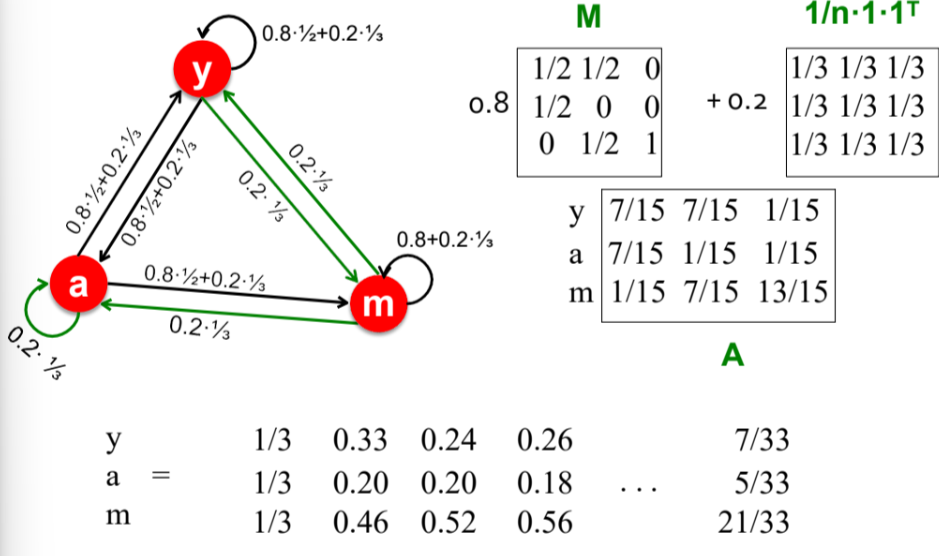
\includegraphics[scale=0.5]{assets/page-rank-random-tp.png}
	\end{center}



	\chapter{Information Filtering e Recommender Systems}
	\section{Introduzione}
	L'Information Filtering è un processo di filtraggio, selezione e organizzazione delle informazioni in base alle preferenze e ai bisogni dell'utente. L'obiettivo principale dell'Information Filtering è fornire all'utente solo le informazioni rilevanti e di qualità, riducendo il rumore e l'informazione inutile. L'Information Filtering è ampiamente utilizzato in diversi contesti, come i motori di ricerca, i social media e i sistemi di raccomandazione. 
	\vspace{\baselineskip}\\
	Un Recommender System è una sottoclasse dei sistemi di Information Filtering che fornisce suggerimenti per item che sono affini ad un particolare utente. Tipicamente, i consigli si riferiscono a diversi processi di decision-making, come ad esempio quale prodotto acquistare, quale musica ascoltare, quale notizia leggere, quale ristorante scegliere, e così via. I Recommender System sono sistemi particolarmente utili quando un utente deve effettuare una scelta su un numero
	di item offerti dal sistema umanamente ingestibile.
	\vspace{\baselineskip}\\
	Vi sono varie definizioni di Recommender System, tra cui:
	\begin{itemize}
		\item Un Recommender System ha l'effetto di guidare l'utente in un processo personalizzato verso oggetti interessanti o utili in un'ampio spazio di scelte.
		\item Un Recommender System fornisce suggerimenti personalizzati sugli elementi che l'utente potrebbe trovare interessanti, abbinando gli elementi ai profili o ai gruppi utente.
		\item Processo di Recommendation: dato un grande set di oggetti e la descrizione dei bisogni dell'utente, l'obiettivo è di mostrare un piccolo set di oggetti che si adattando meglio ai bisogni dell'utente.
		\item Nella sua più comune formulazione, il problema di recommendation è ridotto al problema di stimare ratings per gli oggetti che l'utente non ha ancora valutato.
	\end{itemize}

	\subsection{Information Retrieval vs. Information Filtering}
	Nei sistemi di information retrieval (IR), i bisogni informativi degli utenti sono rappresentati tramite query esplicite, e il sistema si concentra sulla ricerca di informazioni rilevanti all'interno di un vasto insieme di documenti. Tali sistemi, tradizionalmente progettati per un utilizzo ad hoc, sono rivolti a utenti occasionali e non profilati. I database associati erano prevalentemente statici, e l'interazione con l'utente era di natura reattiva, limitata alla selezione degli elementi richiesti.
	\vspace{\baselineskip}\\
	Al contrario, i sistemi di information filtering (IF) e i recommender system non richiedono una query esplicita. Questi sistemi, proattivi per natura, prevedono quali informazioni o item potrebbero interessare all'utente basandosi sul suo comportamento passato, sulle preferenze e su altri fattori. Utilizzano profili dettagliati degli utenti per filtrare gli elementi irrilevanti o raccogliere contenuti rilevanti, facendo affidamento su database molto grandi e dinamici e orientandosi a un utilizzo continuativo da parte di utenti a lungo termine.
	\vspace{\baselineskip}\\
	Negli sviluppi recenti, entrambi i paradigmi hanno subito un'evoluzione significativa. I sistemi di IR hanno integrato caratteristiche orientate a un uso più ripetitivo e prolungato, avvicinandosi a un modello di interazione più personalizzato, mentre i sistemi di IF hanno ulteriormente affinato le tecniche di profilazione e adattamento ai contesti dinamici, consolidando il proprio ruolo nella gestione personalizzata delle informazioni.

	\begin{figure}[H]
		\begin{subfigure}{0.3\textwidth}
			\centering
			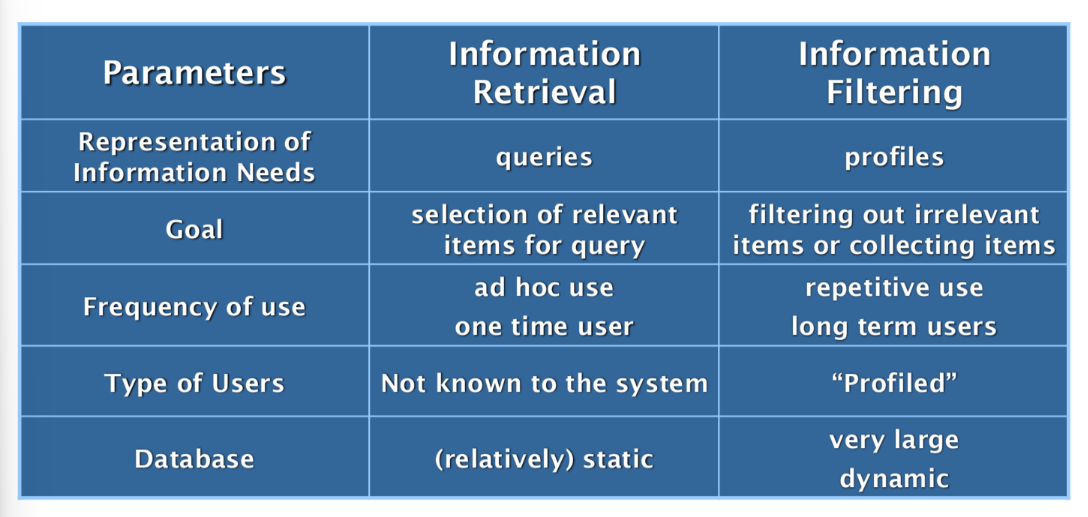
\includegraphics[scale=0.3]{assets/ir-vs-if-2001.png}
			\caption{IR vs. IF - 2000s}
			\label{fig:immagine1}
		\end{subfigure}
		\hspace{0.2\textwidth}
		\begin{subfigure}{0.3\textwidth}
			\centering
			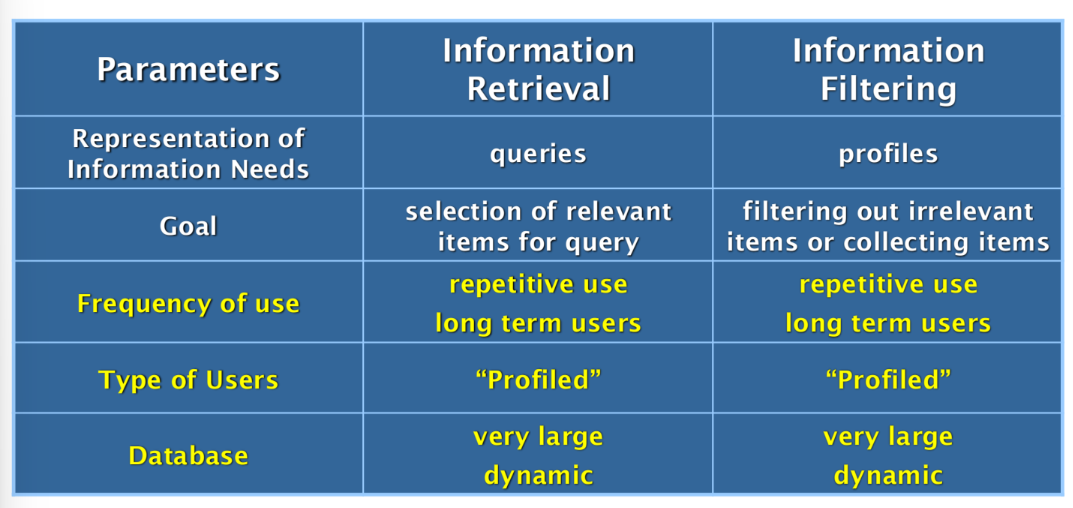
\includegraphics[scale=0.3]{assets/ir-vs-if-oggi.png}
			\caption{IR vs. IF - Oggi}
			\label{fig:immagine2}
		\end{subfigure}
	\end{figure}

	\subsection{Information Overload}
	Il bisogno di progettare e sviluppare sistemi di Information Filtering e Recommender System è dovuto principalmente al problema dell'Information Overload. L'Information Overload si verifica quando l'utente è esposto a un'eccessiva quantità di informazioni, spesso irrilevanti o inaccurate, rendendo difficile trovare e selezionare le informazioni rilevanti. Questo problema è particolarmente rilevante in contesti in cui l'utente è sommerso da una grande quantità di dati, come ad esempio sui social media, nei motori di ricerca e nei siti di e-commerce.
	\vspace{\baselineskip}\\
	Per affrontare l'Information Overload, è nato il bisogno di filtrare e organizzare le informazioni in modo da fornire all'utente solo le informazioni rilevanti.

	\subsection{Architettura di un Sistema di IF}
	\begin{center}
		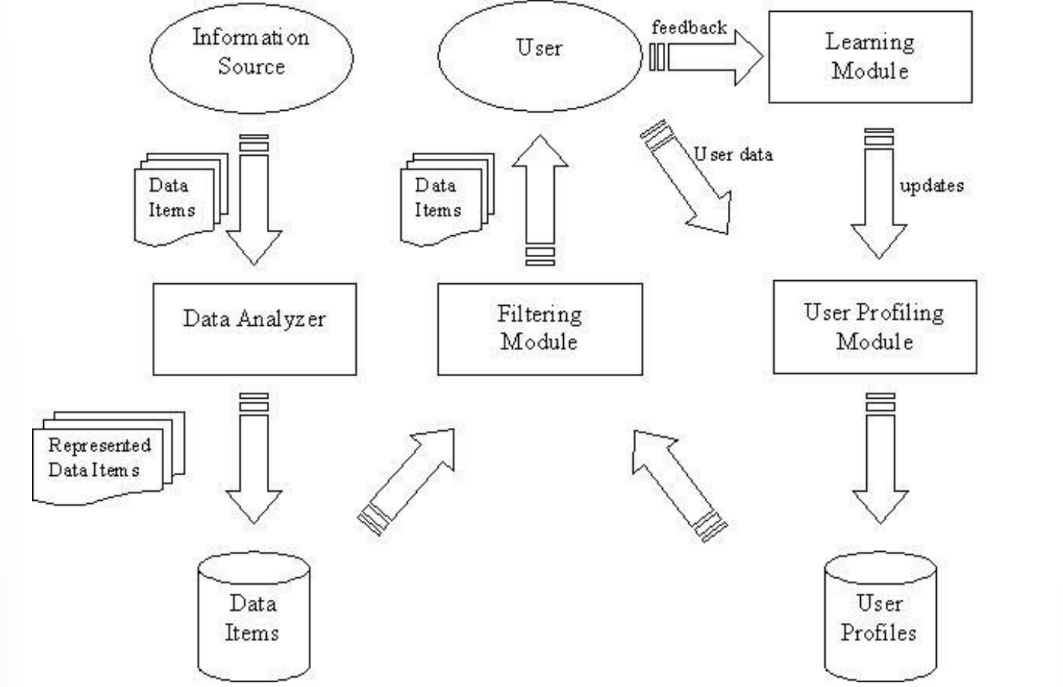
\includegraphics[scale=0.4]{assets/if-arch.png}
	\end{center}
	L'architettura di un sistema di Information Filtering si sviluppa attraverso tre step principali, ciascuno dei quali contribuisce al funzionamento complessivo del sistema.

	\subsection*{Step 1: Building Catalogue}
	Il primo step è dedicato alla costruzione del catalogo di informazioni. In questa fase, le \emph{fonti di informazione} forniscono dati grezzi, denominati \emph{Data Items}, che vengono raccolti e analizzati da un modulo specifico chiamato \emph{Data Analyzer}. Questo modulo ha il compito di elaborare i dati grezzi, rappresentandoli in un formato organizzato e strutturato, noto come \emph{Represented Data Items}. I dati così analizzati vengono successivamente memorizzati in un database centrale, denominato \emph{Data Items}, per poter essere utilizzati nelle fasi successive.
	
	\subsection*{Step 2: Profiling}
	Il secondo step riguarda la costruzione del profilo utente. In questa fase, il sistema raccoglie informazioni direttamente dall'utente attraverso il feedback fornito e le interazioni con il sistema. Queste informazioni vengono elaborate dal modulo di \emph{Learning}, che ha il compito di aggiornare i profili utente in base alle preferenze osservate. I profili così aggiornati vengono archiviati in un database dedicato, denominato \emph{User Profiles}. Questo processo consente di costruire un modello dettagliato e dinamico delle preferenze e dei comportamenti dell'utente.
	
	\subsection*{Step 3: Recommendation}
	Il terzo e ultimo step si concentra sulla generazione di raccomandazioni personalizzate. In questa fase, i dati strutturati memorizzati nel database \emph{Data Items} vengono combinati con le informazioni dei profili utente presenti nel database \emph{User Profiles}. Questo processo avviene grazie al \emph{Filtering Module}, che elabora tali informazioni per produrre raccomandazioni su misura per ciascun utente. Le raccomandazioni vengono quindi presentate all'utente, che ha la possibilità di fornire un feedback. Questo feedback viene nuovamente utilizzato dal sistema per migliorare il processo di apprendimento e affinare ulteriormente le raccomandazioni future.

	\section{Problema di Recommendation}
	Il problema di recommendation è un problema di Machine Learning che si concentra sullo stimare una funzione di utility per predire automaticamente quanto un utente gradirà un item che non ha ancora valutato o che gli è sconosciuto. Dati:
	\[
	\begin{array}{l}
		\text{un insieme di utenti }U = \{u_1, u_2, \ldots, u_M\}\\
		\text{un insieme di item }X = \{x_1, x_2, \ldots, x_N\}\\
		\text{la funzione di utility }f: U \times X \rightarrow R
	\end{array}
	\]
	Lo scopo è di ottenere la stima massima della funzione di utility $f$ per tutti gli item non valutati da ciascun utente:
	\[
		\forall u \in U, x'_u = \arg\max_{x \in X} f(u, x)
	\]

	\subsection{Matrice di Rating}
	Il problema di recommendation può essere rappresentato attraverso una matrice di rating $R$ di dimensione $M \times N$, dove $M$ è il numero di utenti appartenenti all'insieme $U$ e $N$ è il numero di item appartenenti all'insieme $X$. Ogni cella $r_{ij}$ della matrice rappresenta il rating assegnato dall'utente $u_i$ all'item $x_j$. Se l'utente $u_i$ non ha valutato l'item $x_j$, la cella $r_{ij}$ è vuota o contiene un valore nullo.
	\begin{table}[H]
		\begin{tabular}{lllllll}
		 &
		  The Matrix &
		  Titanic &
		  I love shopping &
		  Argo &
		  Love Actually &
		  The hangover \\ \cline{2-7} 
		\multicolumn{1}{l|}{Tommaso} &
		  \multicolumn{1}{l|}{5} &
		  \multicolumn{1}{l|}{1} &
		  \multicolumn{1}{l|}{2} &
		  \multicolumn{1}{l|}{4} &
		  \multicolumn{1}{l|}{3} &
		  \multicolumn{1}{l|}{\color{red}?} \\ \cline{2-7} 
		\multicolumn{1}{l|}{Francesco} &
		  \multicolumn{1}{l|}{2} &
		  \multicolumn{1}{l|}{4} &
		  \multicolumn{1}{l|}{5} &
		  \multicolumn{1}{l|}{3} &
		  \multicolumn{1}{l|}{5} &
		  \multicolumn{1}{l|}{2} \\ \cline{2-7} 
		\multicolumn{1}{l|}{Vito} &
		  \multicolumn{1}{l|}{4} &
		  \multicolumn{1}{l|}{3} &
		  \multicolumn{1}{l|}{2} &
		  \multicolumn{1}{l|}{4} &
		  \multicolumn{1}{l|}{1} &
		  \multicolumn{1}{l|}{3} \\ \cline{2-7} 
		\multicolumn{1}{l|}{Walter} &
		  \multicolumn{1}{l|}{3} &
		  \multicolumn{1}{l|}{5} &
		  \multicolumn{1}{l|}{1} &
		  \multicolumn{1}{l|}{5} &
		  \multicolumn{1}{l|}{2} &
		  \multicolumn{1}{l|}{4} \\ \cline{2-7} 
		\multicolumn{1}{l|}{Cataldo} &
		  \multicolumn{1}{l|}{4} &
		  \multicolumn{1}{l|}{4} &
		  \multicolumn{1}{l|}{5} &
		  \multicolumn{1}{l|}{3} &
		  \multicolumn{1}{l|}{5} &
		  \multicolumn{1}{l|}{2} \\ \cline{2-7} 
		\end{tabular}
	\end{table}
	Al problema di partenza, si aggiunge il problema della \textbf{sparsità} della matrice di rating. La matrice di rating è sparsa quando la maggior parte delle celle è vuota o contiene un valore nullo. 
	\begin{table}[H]
		\begin{tabular}{lllllll}
		 &
			The Matrix &
			Titanic &
			I love shopping &
			Argo &
			Love Actually &
			The hangover \\ \cline{2-7} 
		\multicolumn{1}{l|}{Tommaso} &
			\multicolumn{1}{l|}{5} &
			\multicolumn{1}{l|}{1} &
			\multicolumn{1}{l|}{\color{red}?} &
			\multicolumn{1}{l|}{\color{red}?} &
			\multicolumn{1}{l|}{\color{red}?} &
			\multicolumn{1}{l|}{\color{red}?} \\ \cline{2-7} 
		\multicolumn{1}{l|}{Francesco} &
			\multicolumn{1}{l|}{\color{red}?} &
			\multicolumn{1}{l|}{\color{red}?} &
			\multicolumn{1}{l|}{5} &
			\multicolumn{1}{l|}{3} &
			\multicolumn{1}{l|}{5} &
			\multicolumn{1}{l|}{2} \\ \cline{2-7} 
		\multicolumn{1}{l|}{Vito} &
			\multicolumn{1}{l|}{4} &
			\multicolumn{1}{l|}{3} &
			\multicolumn{1}{l|}{\color{red}?} &
			\multicolumn{1}{l|}{\color{red}?} &
			\multicolumn{1}{l|}{\color{red}?} &
			\multicolumn{1}{l|}{\color{red}?} \\ \cline{2-7} 
		\multicolumn{1}{l|}{Walter} &
			\multicolumn{1}{l|}{3} &
			\multicolumn{1}{l|}{\color{red}?} &
			\multicolumn{1}{l|}{1} &
			\multicolumn{1}{l|}{\color{red}?} &
			\multicolumn{1}{l|}{2} &
			\multicolumn{1}{l|}{4} \\ \cline{2-7} 
		\multicolumn{1}{l|}{Cataldo} &
			\multicolumn{1}{l|}{4} &
			\multicolumn{1}{l|}{4} &
			\multicolumn{1}{l|}{\color{red}?} &
			\multicolumn{1}{l|}{\color{red}?} &
			\multicolumn{1}{l|}{\color{red}?} &
			\multicolumn{1}{l|}{2} \\ \cline{2-7} 
		\end{tabular}
	\end{table}
	Questo problema è comune nei sistemi di recommendation, poiché gli utenti tendono a valutare solo una piccola frazione degli item disponibili. La sparsità della matrice di rating può influenzare negativamente le prestazioni dei Recommender System, poiché rende difficile stimare i rating mancanti e generare raccomandazioni accurate. Nel dettaglio, la sparsità della matrice di rating è calcolata come:
	\[
	\text{Sparsity} = 1 - \frac{|R|}{|X| \times |U|}
	\]
	I ratings possono essere espliciti o impliciti. I ratings espliciti sono valutazioni numeriche assegnate dagli utenti agli item, mentre i ratings impliciti sono informazioni indirette sulle preferenze degli utenti, come ad esempio il tempo trascorso su una pagina web o il numero di click su un link.

	\section{Tecniche di Recommendation}
	Esistono diverse tecniche per affrontare il problema di recommendation, ciascuna delle quali si basa su un approccio specifico per stimare i rating mancanti e generare raccomandazioni personalizzate. Le principali tecniche di recommendation includono:
	\begin{itemize}
		\item \textbf{Content-Based Filtering}: si basa sull'analisi dei contenuti degli item e dei profili utente per generare raccomandazioni personalizzate. Questo approccio utilizza informazioni dettagliate sugli item e sulle preferenze degli utenti per stimare i rating mancanti e suggerire item simili a quelli già valutati positivamente dall'utente.
		\item \textbf{Collaborative Filtering}: si basa sull'analisi delle interazioni tra gli utenti e gli item per generare raccomandazioni personalizzate. Questo approccio utilizza i rating assegnati dagli utenti agli item per identificare pattern comuni e suggerire item che sono stati valutati positivamente da utenti con gusti simili. 
		\item \textbf{Demographic Filtering}: si basa sull'analisi delle caratteristiche demografiche degli utenti per generare raccomandazioni personalizzate. Questo approccio utilizza informazioni dettagliate sugli utenti, come l'età, il genere e la posizione geografica, per identificare gruppi omogenei e suggerire item adatti alle preferenze di ciascun gruppo.
		\item \textbf{Knowledge-Based Filtering}: si basa sull'analisi delle conoscenze esplicite degli utenti per generare raccomandazioni personalizzate. Questo approccio utilizza informazioni dettagliate sulle conoscenze e le competenze degli utenti per identificare item rilevanti e suggerire contenuti educativi e informativi.
		\item \textbf{Community-Based Filtering}: si basa sull'analisi delle interazioni sociali tra gli utenti per generare raccomandazioni personalizzate. Questo approccio utilizza le relazioni sociali e le connessioni tra gli utenti per identificare pattern comuni e suggerire item che sono stati valutati positivamente dai membri della comunità.
		\item \textbf{Hybrid Filtering}: si basa sull'integrazione di diverse tecniche di recommendation per generare raccomandazioni personalizzate. Questo approccio combina i vantaggi di diverse tecniche di recommendation per migliorare la qualità e la precisione delle raccomandazioni, adattandosi alle preferenze e ai bisogni specifici degli utenti.
	\end{itemize}

	\section{Collaborative Filtering}
	Nella vita quotidiana, le persone spesso si affidano ai consigli di amici, familiari o colleghi per prendere decisioni informate su cosa acquistare, cosa guardare o cosa ascoltare. Questo approccio si basa sull'idea che le persone con gusti simili tendano a condividere opinioni e preferenze simili su determinati argomenti.
	\begin{center}
		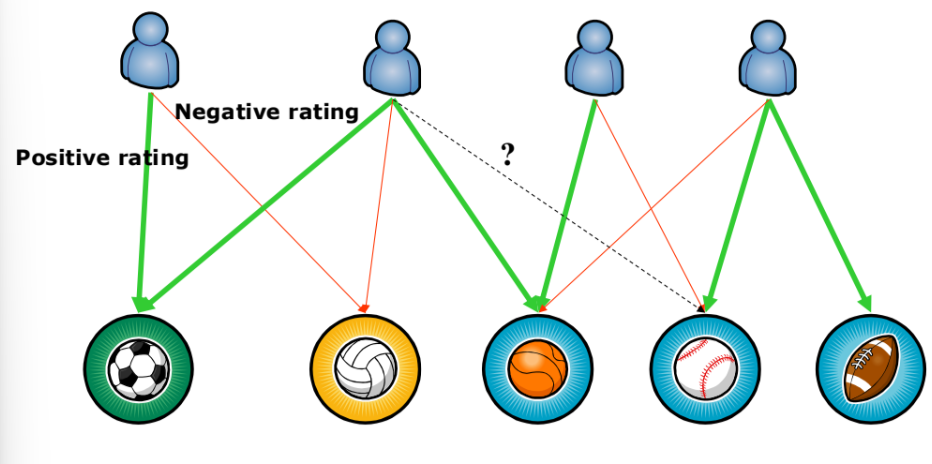
\includegraphics[scale=0.4]{assets/cf-idea.png}
	\end{center}
	Il Collaborative Filtering è un'implementazione computazionale di questo concetto, che si basa sull'analisi delle interazioni tra gli utenti e gli item per identificare pattern comuni e suggerire item che sono stati valutati positivamente da utenti con gusti simili. Si basa, quindi, sull'utilizzo della conoscenza degli utenti, mediante valutazioni implicite o esplicite, per generare raccomandazioni personalizzate. L'idea di partenza è quella di predire quale sarà l'opinione di un utente su un item o diversi items, andando a raccomandare i migliori items per quell'utente.
	\vspace{\baselineskip}\\
	Il collaborative filtering è una metodologia che necessita una infrastruttura di rete che renda possibile la raccolta delle valutazioni degli utenti i quali fruiranno di un servizio web. Si tratta di un sistema distribuito che permette di raccogliere le valutazioni degli utenti e di fornire raccomandazioni personalizzate. Il primo esempio di una applicazione web per il collaborative filtering è MovieLens, un sistema di raccomandazione di film basato sulle valutazioni degli utenti.  
	
	\subsection{Definizione del Problema}
	Il collaborative filtering è una tecnica che si basa su diversi elementi chiave per prevedere il gradimento di un utente verso un determinato oggetto, anche se non ha mai interagito direttamente con esso. La base di partenza è costituita da un insieme di $m$ utenti e un insieme di $n$ items. Ogni utente può aver espresso la propria opinione su uno o più item, tramite valutazioni esplicite, come punteggi numerici, oppure in modo implicito, attraverso comportamenti come l'acquisto o la visualizzazione.
	\vspace{\baselineskip}\\
	Un aspetto centrale del filtraggio collaborativo è l'identificazione di un utente specifico, detto "active user", per il quale si cerca di effettuare la previsione. Per farlo, viene utilizzata una metrica che misura la similarità tra gli utenti, permettendo di individuare un sottogruppo di vicini, ossia utenti con preferenze simili. Questi vicini rappresentano un punto di riferimento per prevedere quale valutazione l'utente attivo potrebbe assegnare a oggetti con cui non ha ancora interagito. 

	\subsection{User-based Nearest-Neighbor Collaborative Filtering}
	Lo User-based Nearest-Neighbor Collaborative Filtering si fonda sull'idea che le preferenze espresse da utenti con gusti simili possano essere utilizzate per effettuare previsioni su nuovi elementi. Questo approccio utilizza come input una matrice di valutazioni utenti-oggetti, e produce come output due possibili risultati: una previsione numerica che indica il grado di gradimento dell'utente per un determinato oggetto, oppure una lista dei migliori $N$ oggetti raccomandati. Il metodo consiste nell'individuare un utente attivo, ad esempio Alice, e un oggetto che Alice non ha ancora valutato. Per effettuare la previsione, si seleziona un gruppo di vicini, ovvero utenti che hanno mostrato gusti simili ad Alice e che hanno valutato l'oggetto in questione. La previsione viene quindi calcolata utilizzando metriche come, ad esempio, la media delle valutazioni dei vicini per quell'oggetto. Questo processo si ripete per tutti gli oggetti non valutati da Alice, generando così un insieme di raccomandazioni personalizzate. L'approccio si basa su due assunti principali: innanzitutto, si suppone che utenti con gusti simili nel passato continueranno ad avere preferenze simili anche in futuro. In secondo luogo, si assume che le preferenze degli utenti rimangano stabili nel tempo.

	\begin{tcolorbox}[title=Esempio]
		Consideriamo un esempio concreto: una tabella che rappresenta le valutazioni assegnate da Alice e da altri utenti a un insieme di oggetti. Il compito è prevedere il gradimento di Alice per \textit{Item5}, che non è stato ancora valutato. La tabella delle valutazioni è la seguente:

		\begin{table}[H]
			\centering
			\begin{tabular}{|c|c|c|c|c|c|}
				\hline
				& \textbf{Item1} & \textbf{Item2} & \textbf{Item3} & \textbf{Item4} & \textbf{Item5} \\ \hline
				\textbf{Alice} & 5 & 3 & 4 & 4 & \color{red}? \\ \hline
				\textbf{User1} & 3 & 1 & 2 & 3 & 3 \\ \hline
				\textbf{User2} & 4 & 3 & 4 & 3 & 5 \\ \hline
				\textbf{User3} & 3 & 3 & 1 & 5 & 4 \\ \hline
				\textbf{User4} & 1 & 5 & 5 & 2 & 1 \\ \hline
			\end{tabular}
		\end{table}
	\end{tcolorbox}
	Per prevedere se Alice gradirà o meno \textit{Item5}, il metodo richiede di affrontare alcune domande fondamentali:
	\begin{itemize}
		\item Come misurare la similarità tra gli utenti?
		\item Quanti vicini considerare per la previsione?
		\item Come generare una previsione basandosi sulle valutazioni dei vicini?
	\end{itemize}
	La similarità tra utenti può essere calcolata utilizzando diverse metriche. Una delle più comuni è il \textbf{coefficiente di correlazione di Pearson}, che misura la relazione lineare tra le valutazioni di due utenti. Nello specifico, la similarità tra due utenti \(a\) e \(b\) è calcolata come segue:
	\[
	\text{sim}(a, b) = \frac{\sum_{p \in P} (r_{a,p} - \bar{r}_a)(r_{b,p} - \bar{r}_b)}{\sqrt{\sum_{p \in P} (r_{a,p} - \bar{r}_a)^2} \sqrt{\sum_{p \in P} (r_{b,p} - \bar{r}_b)^2}}
	\]
	dove:
	\begin{itemize}
		\item \(r_{a,p}\): è la valutazione dell'utente \(a\) per l'elemento \(p\).
		\item \(\bar{r}_a\): è la media delle valutazioni dell'utente \(a\).
		\item \(P\): è l'insieme degli elementi valutati sia dall'utente \(a\) che dall'utente \(b\).
		\item \(\text{sim}(a, b)\): rappresenta il grado di similarità tra i due utenti, con valori compresi tra \(-1\) (anti-correlazione totale) e \(1\) (correlazione perfetta).
	\end{itemize}
	Questa formula tiene conto non solo delle valutazioni, ma anche delle differenze nei comportamenti di valutazione tra gli utenti.
	\vspace{\baselineskip}\\
	Un'altra metrica comunemente utilizzata è la similarità basata sul coseno, che misura l'angolo tra i vettori delle valutazioni degli utenti. Questa metrica si concentra sulla direzione dei pattern di valutazione, ignorando le differenze medie.
	\vspace{\baselineskip}\\
	Dopo aver calcolato la similarità tra l'utente attivo e i suoi vicini, è possibile prevedere la valutazione mancante per un determinato elemento. La previsione tiene conto delle valutazioni fornite dai vicini e delle loro similarità con l'utente attivo, ponderando ciascun contributo in base a quanto siano vicini o simili. La formula comunemente utilizzata per calcolare la previsione è la seguente:
	\[
	\text{pred}(a,p) = \bar{r}_a + \frac{\sum_{b \in N} \text{sim}(a, b) \cdot (r_{b,p} - \bar{r}_b)}{\sum_{b \in N} |\text{sim}(a, b)|}
	\]
	dove:
	\begin{itemize}
		\item \(a\): L'utente attivo per il quale si vuole calcolare la previsione.
		\item \(p\): L'elemento per il quale si vuole prevedere la valutazione.
		\item \(\bar{r}_a\): La media delle valutazioni fornite dall'utente attivo \(a\), usata per normalizzare il risultato e tenere conto del suo stile di valutazione.
		\item \(N\): L'insieme dei vicini considerati, cioè gli utenti con valutazioni simili a quelle dell'utente attivo.
		\item \(\text{sim}(a, b)\): La similarità tra l'utente attivo \(a\) e un vicino \(b\), calcolata con una metrica come il coefficiente di correlazione di Pearson.
		\item \(r_{b,p}\): La valutazione che il vicino \(b\) ha dato all'elemento \(p\).
		\item \(\bar{r}_b\): La media delle valutazioni fornite dal vicino \(b\), utilizzata per normalizzare il suo contributo.
	\end{itemize}
	Questa formula calcola la previsione per l'utente attivo \(a\) e l'elemento \(p\) come la somma della media delle valutazioni di \(a\) e di un contributo ponderato dei vicini, normalizzato per la somma delle similarità assolute. Questo processo permette di generare previsioni personalizzate, basate sul comportamento dei vicini e sullo stile di valutazione dell'utente attivo. Nello specifico, il processo di previsione si articola nei seguenti passaggi:
	\begin{enumerate}
		\item \textbf{Calcolo del contributo dei vicini:}  
		Per ciascun vicino \(b \in N\), si calcola la differenza tra la sua valutazione per l'elemento \(p\) (\(r_{b,p}\)) e la sua media delle valutazioni (\(\bar{r}_b\)). Questo passo permette di comprendere quanto il vicino valuti l'elemento \(p\) rispetto al suo stile di valutazione generale.
		
		\item \textbf{Ponderazione tramite similarità:}  
		Il contributo di ciascun vicino viene moltiplicato per la similarità \(\text{sim}(a, b)\) tra l'utente attivo e il vicino. I vicini con una similarità più alta avranno un peso maggiore nella previsione.
		
		\item \textbf{Normalizzazione:}  
		La somma dei contributi ponderati viene divisa per la somma dei valori assoluti delle similarità \(|\text{sim}(a, b)|\). Questo passaggio assicura che la previsione non sia influenzata in modo sproporzionato da vicini con similarità molto alta o molto bassa.
		
		\item \textbf{Aggiunta della media dell'utente attivo:}  
		Alla fine, si aggiunge \(\bar{r}_a\), la media delle valutazioni dell'utente attivo. Questo riporta il risultato nel contesto dello stile di valutazione generale dell'utente, rendendo la previsione più coerente con il suo comportamento.
	\end{enumerate}
	Per migliorare la qualità delle previsioni, si possono adottare alcune strategie:
	\begin{itemize}
		\item \textbf{Valutazione del numero di elementi co-valutati:} più elementi comuni portano a stime più affidabili. 
		Una possibile soluzione è l'utilizzo di un "significance weighting", che riduce linearmente il peso quando il numero di elementi co-valutati è basso. Si può penalizzare la similarità tra utenti o tra elementi utilizzando un fattore proporzionale al numero di oggetti comuni valutati, nel caso in cui tale numero sia inferiore a un valore soglia $\gamma > 0$:
		\[
		w'_{uv} = \frac{\min{|I_{uv}|, \gamma}}{\gamma} \cdot w_{uv}
		\]
		dove $|I_{uv}|$ è il numero di oggetti co-valutati da $u$ e $v$, e $w_{uv}$ è la similarità tra i due utenti. Analogamente, per la similarità tra elementi:
		\[
		w'_{ij} = \frac{\min{|U_{ij}|, \gamma}}{\gamma} \cdot w_{ij}
		\]
		dove $|U_{ij}|$ è il numero di utenti che hanno valutato entrambi gli oggetti $i$ e $j$.
	
		\item \textbf{Peso alle valutazioni con maggiore varianza:} elementi su cui gli utenti differiscono maggiormente possono essere più informativi. Non tutte le valutazioni dei vicini potrebbero essere ugualmente "valide". L'accordo su elementi molto popolari è meno informativo rispetto all'accordo su elementi controversi. Una possibile soluzione è attribuire un peso maggiore agli elementi con una varianza più alta, utilizzando il concetto di \textit{Inverse User Frequency} (IUF). 
		Il peso $\lambda_i$ di un elemento $i$ può essere calcolato come:
		\[
		\lambda_i = \log \frac{|U|}{|U_i|}
		\]
		dove $|U|$ è il numero totale di utenti e $|U_i|$ è il numero di utenti che hanno valutato l'elemento $i$. Questo peso può essere utilizzato, ad esempio, nel calcolo della \textit{Frequency-Weighted Pearson Correlation} (FWPC) tra due utenti $u$ e $v$, dove:
		\[
		FWPC(u, v) = \frac{\sum_{i \in I_{uv}} \lambda_i (r_{ui} - \bar{r}_u)(r_{vi} - \bar{r}_v)}{\sqrt{\sum_{i \in I_{uv}} \lambda_i (r_{ui} - \bar{r}_u)^2} \sqrt{\sum_{i \in I_{uv}} \lambda_i (r_{vi} - \bar{r}_v)^2}}
		\]
	
		\item \textbf{Amplificazione dei casi:} dare più peso ai vicini con alta similarità.
		\item \textbf{Selezione del vicinato:} considerare solo un sottoinsieme di vicini particolarmente rilevanti.
	\end{itemize}
	Lo User Based CF è un approccio detto \textit{memory-based}, poiché si basa direttamente sui dati di valutazione degli utenti per generare raccomandazioni. Questo approccio è semplice e intuitivo, ma può essere computazionalmente costoso, specialmente con un numero elevato di utenti e oggetti. Inoltre, non rappresenta una soluzione per la maggior parte degli scenari reali. Per affrontare queste limitazioni, è possibile utilizzare un approccio \textit{model-based}, che si basa su modelli statistici o di machine learning per pre-processare i dati e, al momento dell'esecuzione, utilizzare solamente i modelli addestrati per generare raccomandazioni. Qesti modelli vengono ri-addestrati e aggiornati periodicamente per mantenere la loro accuratezza e adattarsi ai cambiamenti nelle preferenze degli utenti, nonostante sia computazionalmente costoso. Un'esempio di approccio model-based è l'\textbf{Item-based Collaborative Filtering}.

	\subsection{Item-based Collaborative Filtering}
	L'approccio Item-based Collaborative Filtering si basa sull'idea che gli item simili tendano ad essere valutati in modo simile dagli utenti. Di conseguenza, la similarità tra item può essere utilizzata per prevedere il gradimento di un utente per un determinato item, anche se non ha mai interagito direttamente con esso. Questo approccio è stato formalizzato per ridurre la complessità del calcolo della similarità tra utenti, concentrandosi invece sulla similarità tra item, considerando che il numero di item è generalmente inferiore al numero di utenti.
	\vspace{\baselineskip}\\
	La metrica utilizzata per il calcolo della similarità tra item è spesso la similarità del coseno:
	\[
		\text{sim}(\overrightarrow{a}, \overrightarrow{b}) = \frac{\overrightarrow{a} \cdot \overrightarrow{b}}{\|\overrightarrow{a}\| \cdot \|\overrightarrow{b}\|}
	\]
	talvolta normalizzata e modificata per prendere in considerazione la media dei rating dell'utente. In questo modo si ottiene la Adjusted Cosine Similarity:
	\[
		\text{sim}(\overrightarrow{a}, \overrightarrow{b}) = \frac{\sum_{u \in U} (r_{u,a} - \bar{r}_u)(r_{u,b} - \bar{r}_u)}{\sqrt{\sum_{u \in U} (r_{u,a} - \bar{r}_u)^2} \sqrt{\sum_{u \in U} (r_{u,b} - \bar{r}_u)^2}}
	\]
	dove:
	\begin{itemize}
		\item \(r_{u,a}\) e \(r_{u,b}\) sono i rating degli utenti \(u\) per gli item \(a\) e \(b\).
		\item \(\bar{r}_u\) è la media dei rating dell'utente \(u\).
		\item \(U\) è l'insieme degli utenti che hanno valutato sia l'item \(a\) che l'item \(b\).
	\end{itemize}
	Una volta calcolata la similarità tra item, è possibile prevedere il gradimento di un utente per un determinato item utilizzando una formula simile a quella utilizzata nello User-based Collaborative Filtering:
	\[
		\text{pred}(u, p) = \frac{\sum_{i \in ratedItem(u)} sim(i,p) \times r_{u,i}}{\sum_{i \in ratedItem(u)} sim(i,p)}
	\]
	Solitamente, non tutti i vicini sono presi in considerazione per il calcolo della previsione, ma solo i \(k\) item più simili a \(p\). Questo permette di ridurre la complessità computazionale e di concentrarsi sui vicini più rilevanti.

	\subsection{Ratings Impliciti e Espliciti}
	Le valutazioni degli utenti possono essere esplicite o implicite. I ratings espliciti sono valutazioni numeriche assegnate dagli utenti agli item, mentre i ratings impliciti sono informazioni indirette sulle preferenze degli utenti, come ad esempio il tempo trascorso su una pagina web o il numero di click su un link. I ratings espliciti sono generalmente più facili da interpretare e precisi per l'inferenza delle preferenze degli utenti, ma possono essere soggetti a bias e manipolazioni. Inoltre, l'utente potrebbe non essere disposto a fornire valutazioni esplicite per tutti gli item, rendendo difficile stimare i rating mancanti e generare raccomandazioni accurate. I ratings impliciti, d'altra parte, sono spesso più facili da raccogliere e possono fornire informazioni preziose sulle preferenze degli utenti, ma possono essere soggetti a rumore e ambiguità. Inoltre, l'interpretazione dei ratings impliciti può essere più complessa e soggetta a interpretazioni errate. In generale, ratings espliciti ed impliciti possono essere utilizzati insieme per migliorare la qualità e la precisione delle raccomandazioni, adattandosi alle preferenze e ai bisogni specifici degli utenti.

	\subsection{Sparsità dei dati}
	Il \textbf{problema della sparsità} è un aspetto critico nelle raccomandazioni, in quanto la matrice di rating è spesso molto sparsa, il che rende difficile stimare i rating mancanti e generare raccomandazioni accurate. Questo fenomeno è amplificato dal \textbf{problema del Cold Start}, che si verifica quando nuovi utenti o nuovi item non hanno sufficienti dati di interazione, contribuendo ulteriormente alla scarsità di informazioni. Il Cold Start si suddivide in due situazioni principali: il \textbf{New Item Cold Start}, in cui i nuovi item non hanno valutazioni da parte degli utenti, rendendo difficile stimare i rating mancanti e generare raccomandazioni accurate, e il \textbf{New User Cold Start}, in cui i nuovi utenti non hanno ancora valutato alcun item, il che rende difficile identificare pattern comuni e suggerire item che sono stati valutati positivamente da utenti con gusti simili. Inoltre, esiste il \textbf{Grey Sheep Problem}, che riguarda gli utenti con un numero insufficiente di valutazioni per identificare pattern comuni, complicando ulteriormente la generazione di raccomandazioni personalizzate.
	\vspace{\baselineskip}\\
	Per affrontare il problema della sparsità, è possibile utilizzare diverse strategie, come il forzare l'utente a valutare un certo numero di item prima di ricevere raccomandazioni, o l'assegnare valutazioni di default agli item che sono stati valutati solo da uno dei due utenti coinvolti, altrimenti per la fase iniziale si potrebbe utilizzare un approccio diverso, come il Content-Based Filtering. 

	\subsection{Vantaggi}
	\begin{itemize}
		\item \textbf{Semplicità}: I sistemi di raccomandazione collaborativa sono relativamente semplici da implementare e non richiedono una conoscenza approfondita del contenuto degli item. Inoltre non necessitano di ingegnerizzare la conoscenza degli item.
		\item \textbf{Personalizzazione}: Le raccomandazioni sono personalizzate in base alle preferenze degli utenti, migliorando l'esperienza dell'utente.
		\item \textbf{Adattabilità}: I sistemi di raccomandazione collaborativa possono adattarsi rapidamente ai cambiamenti nelle preferenze degli utenti, fornendo raccomandazioni aggiornate e rilevanti.
	\end{itemize}
	\subsection{Svantaggi}
	\begin{itemize}
		\item \textbf{Problema della Sparsità}
		\item \textbf{Problema della Scalabilità}: Sebbene i sistemi di raccomandazione collaborativa siano scalabili, il calcolo delle similarità tra utenti o item può diventare computazionalmente costoso con l'aumentare del numero di utenti e item.
		\item \textbf{Assenza di Trasparenza nelle Raccomandazioni}: Le raccomandazioni sono generate automaticamente in base alle interazioni degli utenti, senza fornire spiegazioni dettagliate sulle ragioni alla base delle raccomandazioni.
	\end{itemize}

	\section{Content-Based Filtering}
	I Content-Based Recommendation Systems sono ampiamente utilizzati per generare raccomandazioni personalizzate, basandosi sull'analisi dei contenuti degli item e dei profili utente. A differenza dei sistemi di Collaborative Filtering, che dipendono dalla disponibilità di una comunità, i sistemi Content-Based si concentrano sulle descrizioni degli item, che devono essere strutturate e uniformi. Questi item vengono rappresentati tramite attributi specifici (ad esempio, Titolo, Genere, Autore, Prezzo, Trama per i libri) e ogni caratteristica viene associata a un insieme finito di valori, creando una rappresentazione vettoriale, spesso booleana. La comparazione tra il contenuto degli item e il profilo utente, che include preferenze esplicite o implicite, permette di generare raccomandazioni personalizzate. Il processo di filtraggio si basa su metodi come il confronto di stringhe o la similarità testuale, spesso ispirati dall'Information Retrieval. I sistemi Content-Based possono essere Heuristic-Based, utilizzando tecniche di information retrieval, o Model-Based, impiegando metodi di machine learning per stimare i rating mancanti e affinare ulteriormente le raccomandazioni.

	\subsection{Architettura CBRS}
	\begin{center}
		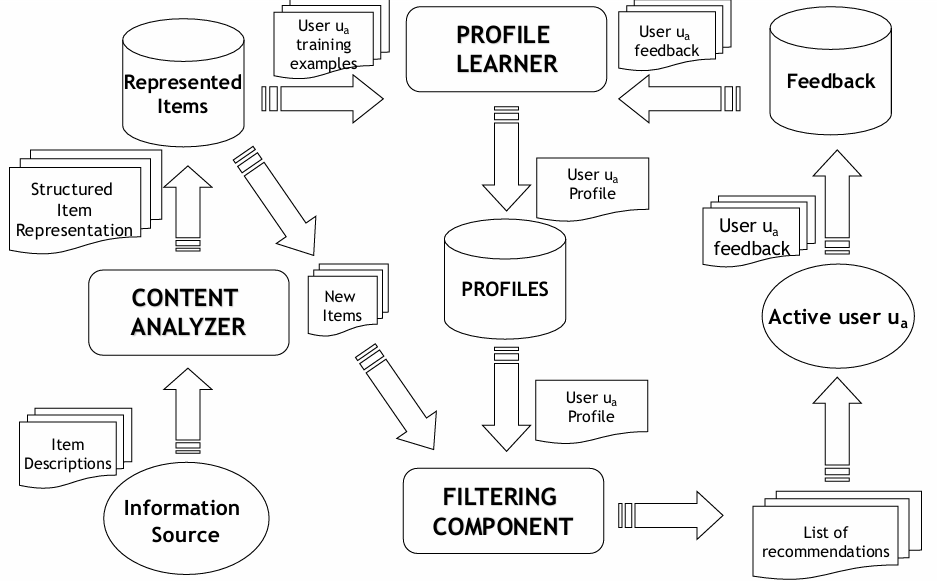
\includegraphics[scale=0.4]{assets/cbrs-arch.png}
	\end{center}
	L'architettura di un Content-Based Recommender System (CBRS) si suddivide in tre componenti principali, che lavorano in modo sinergico per assicurare raccomandazioni efficaci: rappresentazione, profiling e raccomandazione.

	La \textbf{fase di rappresentazione} è dedicata alla trasformazione degli oggetti in una forma strutturata. Questo viene realizzato attraverso un modulo chiamato \textit{Content Analyzer}, che prende in ingresso le descrizioni degli oggetti da una fonte informativa. Il Content Analyzer estrae e struttura le caratteristiche rilevanti degli oggetti, generando una rappresentazione standardizzata. Questa rappresentazione costituisce il punto di partenza per il confronto con le preferenze degli utenti e l'elaborazione delle raccomandazioni.

	Successivamente, nella \textbf{fase di profiling}, il sistema costruisce e aggiorna i profili degli utenti. Ogni profilo utente rappresenta le preferenze individuali, basandosi su interazioni passate, feedback fornito o dati espliciti. Il componente principale di questa fase è il \textit{Profile Learner}, che utilizza le informazioni sugli oggetti rappresentati insieme ai feedback degli utenti per generare o perfezionare i profili. Questi profili sono memorizzati e utilizzati per personalizzare le raccomandazioni in base alle preferenze specifiche di ogni utente.

	Infine, nella \textbf{fase di raccomandazione}, il \textit{Filtering Component} confronta il profilo attivo dell'utente con le rappresentazioni degli oggetti disponibili. Sulla base della somiglianza tra il profilo dell'utente e le caratteristiche degli oggetti, viene generata una lista di raccomandazioni personalizzate. Il feedback dell'utente, raccolto durante questa fase, alimenta il processo di aggiornamento dei profili, migliorando progressivamente l'efficacia del sistema.

	\subsection{Metriche di Similarità}
	Considerando che la maggior parte delle tecniche di Content-Based Filtering sono applicate a dati strutturati, quali documenti di testo, e considerando che il requisito alla base dei CBRS è la rappresentazione degli item secondo un insieme di caratteristiche, attributi e keywords, essa viene spesso effettuata tramite tecniche di Information Retrieval. In particolare, per rappresentare gli item e i profili utente, può essere utilizzato il TF-IDF (Term Frequency-Inverse Document Frequency), un metodo standard che trasforma i documenti testuali in vettori numerici multidimensionali, andando a pesare le parole in base alla loro frequenza nei documenti e alla loro rarità nel corpus.
	\vspace{\baselineskip}\\
	Una volta rappresentati gli oggetti tramite TF-IDF, è possibile sfruttare queste rappresentazioni per calcolare la somiglianza tra gli oggetti. Qui entra in gioco il metodo dei \textit{k-nearest neighbors} (k-NN), che utilizza tali rappresentazioni per identificare gli oggetti più vicini a un dato elemento. Il k-NN sfrutta metriche come la similarità coseno per determinare quanto un oggetto sia simile a quelli già valutati dall'utente. Ad esempio, se un utente ha apprezzato libri che condividono parole chiave con un nuovo libro non ancora valutato, il sistema può prevedere che anche quest'ultimo sarà di suo interesse. L'integrazione del TF-IDF con il k-NN consente di migliorare le raccomandazioni, poiché le due tecniche si completano a vicenda. Il TF-IDF fornisce una rappresentazione strutturata e pesata degli oggetti, mentre il k-NN utilizza questa rappresentazione per effettuare predizioni basate sui vicini più simili. Questa combinazione è particolarmente utile per modellare sia interessi a breve termine, come la raccomandazione di sequel o contenuti correlati, sia preferenze a lungo termine, soprattutto se il k-NN è affiancato da altri modelli più sofisticati. In questo modo, il sistema di raccomandazione può offrire suggerimenti dinamici e personalizzati, adattandosi sia alle caratteristiche degli oggetti che ai gusti evolutivi dell'utente.	Anche in questo caso è importante considerare che la similarità coseno non tiene conto delle differenze medie nei rating degli utenti, che possono influenzare le raccomandazioni. Per questo motivo, è preferibile utilizzare la Adjusted Cosine Similarity, che tiene conto delle differenze medie nei rating degli utenti, fornendo raccomandazioni più accurate e personalizzate.
	\vspace{\baselineskip}\\
	Inoltre, tecniche come l'algoritmo di Rocchio possono essere utilizzate per migliorare ulteriormente il processo di raccomandazione. Questo approccio, pensato per problemi di categorizzazione, combina i vettori degli esempi positivi e negativi per generare un vettore prototipo per ciascuna classe (\(D^+\) e \(D^-\)), rappresentando rispettivamente gli item "piaciuti" e "non piaciuti". Utilizzando lo schema di pesatura TF-IDF, l'algoritmo calcola i centroidi di ciascuna classe e determina la rilevanza degli oggetti in base alla distanza dal prototipo, misurata con la similarità coseno. Questo consente di regolare l'importanza relativa di esempi positivi e negativi, migliorando l'accuratezza delle previsioni.  Parallelamente, un altro approccio consiste nell'utilizzo di metodi probabilistici, che trattano il problema come una classica classificazione testuale. Attraverso una rappresentazione booleana degli oggetti e l'applicazione del teorema di Bayes, è possibile calcolare la probabilità che un documento appartenga alla classe "piaciuto" o "non piaciuto". Ad esempio, dati gli attributi di un documento (ad es., \textit{recommender, intelligent, learning, school}), le probabilità condizionate associate vengono combinate per stimare l'appartenenza a una delle due classi.

	\subsection{Limitazioni dei CBRS e possibili soluzioni}
	\subsubsection*{Limitazioni}  
	I metodi di raccomandazione basati sul contenuto (Content-Based Recommendation Systems, CBRS) presentano diverse limitazioni che ne riducono l'efficacia in alcune applicazioni. Innanzitutto, l'utilizzo delle sole parole chiave potrebbe non essere sufficiente per giudicare adeguatamente la qualità o la rilevanza di un documento o di una pagina web. Questo perché le parole chiave non riescono a catturare aspetti come l'aggiornamento dei contenuti, la fruibilità, l'estetica o lo stile di scrittura. Inoltre, il contenuto disponibile potrebbe essere troppo breve o limitato per fornire informazioni utili per la raccomandazione, e in alcuni casi, come per i file multimediali, potrebbe non essere automaticamente estraibile o analizzabile.
	\vspace{\baselineskip}\\
	Un'altra problematica riguarda la fase di inizializzazione, nota anche come \textit{ramp-up phase}, durante la quale è necessario raccogliere una quantità significativa di dati di training per costruire modelli accurati. Questa esigenza rappresenta una sfida, soprattutto per nuovi utenti o sistemi appena avviati. Nell'era del Web 2.0, tuttavia, è possibile integrare dati provenienti da altre fonti, come i social media, per apprendere le preferenze degli utenti, sebbene ciò comporti una maggiore complessità nella progettazione del sistema. 
	\vspace{\baselineskip}\\
	Infine, uno dei problemi più comuni nei metodi basati sul contenuto è il rischio di overspecializzazione. Gli algoritmi tendono infatti a proporre contenuti molto simili a quelli già valutati positivamente dall'utente, limitando la scoperta di nuovi interessi o categorie di contenuti. Questa mancanza di diversificazione può rendere il sistema meno interessante e utile per gli utenti nel lungo termine.   

	\subsubsection*{Possibili soluzioni}
	Per superare le limitazioni dei metodi di raccomandazione basati sul contenuto, sono state proposte diverse soluzioni che puntano a migliorare la rappresentazione degli oggetti e a diversificare i risultati delle raccomandazioni. Un primo problema, relativo alla limitata capacità di analisi dei contenuti, può essere affrontato adottando strategie innovative per rappresentare gli oggetti e i profili degli utenti, andando oltre l'uso delle semplici parole chiave. Questo approccio include l'analisi semantica, che sfrutta fonti di conoscenza esterne come WordNet o Wikipedia per arricchire la rappresentazione degli oggetti con informazioni più profonde e contestualizzate.  
	\vspace{\baselineskip}\\
	Un secondo problema, legato all'overspecializzazione, richiede una diversificazione dei risultati per evitare che gli algoritmi raccomandino sempre e solo contenuti simili a quelli già apprezzati. A tale scopo, si può ricorrere a una maggiore infusione di conoscenza da fonti aperte, il che consente di ampliare lo spettro di contenuti proposti agli utenti, favorendo così la scoperta di nuovi interessi. L'analisi semantica rappresenta uno degli strumenti principali per andare "oltre le parole chiave". Questo approccio si basa su due elementi fondamentali: da un lato, la semantica, che identifica i concetti presenti nei documenti attraverso tecniche avanzate di elaborazione del linguaggio naturale (NLP), superando i limiti delle semplici parole chiave; dall'altro, la personalizzazione, che consente di rappresentare i bisogni informativi degli utenti in modo più efficace, costruendo profili utente profondi e accurati.  
	\vspace{\baselineskip}\\
	Un esempio concreto di questo approccio è la disambiguazione del significato delle parole (\textit{Word Sense Disambiguation}, WSD), che consiste nel selezionare il significato corretto di una parola in base al contesto in cui essa appare. Ad esempio, la parola "Apple" può riferirsi al frutto oppure al marchio di un'azienda tecnologica, e il WSD utilizza risorse come dizionari, ontologie e repository semantici (ad esempio, WordNet) per risolvere tali ambiguità. La WSD non solo permette di rappresentare in modo più preciso gli oggetti, ma affronta anche il problema dell'overspecializzazione. Attraverso l’uso di relazioni semantiche tra i concetti, come quelle offerte da WordNet, è possibile arricchire i profili utente con informazioni che vanno oltre il contenuto immediatamente valutato. Questo processo può essere implementato tramite approcci \textit{knowledge-based}, che utilizzano risorse come dizionari leggibili automaticamente, oppure \textit{corpus-based}, che sfruttano corpora etichettati semanticamente.
	
	\subsection{Profili semantici per i CBRS}
	Per affrontare le limitazioni dei sistemi di raccomandazione basati sul contenuto (CBRS), sono state sviluppate tecniche innovative che integrano analisi semantiche avanzate. Tra queste, l'approccio dei \textit{Sense-Based Profiles} rappresenta una soluzione promettente.	I profili semantici si basano sull'utilizzo di identificatori di senso, come i synset di WordNet, per rappresentare i contenuti e i profili utente. Questo metodo va oltre le semplici parole chiave, fornendo una comprensione più approfondita e contestuale degli oggetti e degli interessi degli utenti. Ad esempio, termini ambigui come "Apple" possono essere disambiguati per distinguere tra il frutto e l'azienda tecnologica.
	L'adozione di profili semantici offre numerosi vantaggi:
	\begin{itemize}
		\item \textbf{Semantic Matching}: consente di calcolare la similarità tra concetti anziché limitarsi a confrontare stringhe di testo. Questo migliora l'accuratezza delle raccomandazioni.
		\item \textbf{Multilinguismo}: i concetti semantici sono indipendenti dalla lingua, garantendo un'applicabilità globale.
		\item \textbf{Trasparenza}: le raccomandazioni possono essere spiegate in termini di concetti condivisi con l'utente.
		\item \textbf{Collaborative Filtering}: i profili semantici consentono di identificare utenti simili anche in assenza di corrispondenze dirette nei contenuti.
	\end{itemize}

	\section{Valutazione dei sistemi di Recommendation}
	Alla base dei sistemi di raccomandazione è presente il perseguimento di due obiettivi: uno per l'erogatore del servizio, che mira a migliorare la soddisfazione dell'utente e a incrementare le vendite, e uno per l'utente, che cerca di ottenere raccomandazioni personalizzate e rilevanti. Nel primo caso, lo scopo fornire un servizio di predizione e persuasione che possa influenzare il comportamento degli utenti. La persuasione ha lo scopo di indurre l'utente a compiere determinate azioni, come l'acquisto di un prodotto o la visualizzazione di un contenuto, andando a raccomandare oggetti che potrebbero essere di interesse per l'utente. La predizione, invece, si concentra sulla stima delle preferenze dell'utente, cercando di prevedere quali oggetti potrebbero essere apprezzati in futuro. Il successo di un Recommender System può essere valutato in maniera diretta o indiretta. Le metriche dirette misurano l'efficacia delle raccomandazioni in base a criteri oggettivi, come il tasso di conversione (il ratio tra il numero di acquisti fatti grazie alle raccomandazioni e il numero totale di raccomandazioni). Le metriche indirette, invece, valutano l'esperienza dell'utente e la qualità delle raccomandazioni in base a criteri soggettivi, come il lift factor (l'incremento delle vendite ottenuto grazie all'introduzione del sistema di raccomandazione). Nel secondo caso, l'obiettivo è fornire all'utente raccomandazioni personalizzate e rilevanti, che rispecchino le sue preferenze e i suoi interessi.

	\subsection{Design Space}
	Per effettuare una valutazione accurata dei sistemi di raccomandazione, è necessario considerare diversi aspetti che compongono il cosiddetto \textit{Design Space}. Questo spazio di progettazione include vari elementi che influenzano l'efficacia e l'usabilità del sistema. Tra questi, i principali sono:
	\begin{itemize}
		\item \textbf{Requisiti funzionali}: comprendono le funzionalità offerte dal sistema, come la generazione di raccomandazioni personalizzate, la previsione delle preferenze dell'utente e la diversificazione dei risultati.
		\item \textbf{Requisiti non funzionali}: riguardano aspetti quali:
		\begin{itemize}
			\item \textbf{Adattabilità}: la capacità del sistema di adattarsi ai cambiamenti nelle preferenze degli utenti, nella disponibilità degli item e nelle condizioni di contesto. Essa dipende dalla fase di addestramento e dalla fase di esecuzione del sistema.
			\item \textbf{Responce Time}: il tempo di risposta del sistema, che deve essere sufficientemente rapido per fornire raccomandazioni in tempo reale.
			\item \textbf{Scalabilità}: la capacità del sistema di gestire grandi quantità di dati, di utenti e di raccomandazioni concorrenti, mantenendo alte prestazioni. E' misurata in termini del numero massimo di raccomandazioni on-line che il sistema può gestire al secondo e può essere misurata solamente con test sperimentali. Un basso response time non implica necessariamente una buona scalabilità.
			\item \textbf{Requisiti Hardware}: includono la potenza di calcolo, la memoria e la larghezza di banda necessarie per eseguire il sistema in modo efficiente. Comprende le scelte architetturali e di carico di lavoro server-side e client-side.
			\item \textbf{Sicurezza}: la protezione dei dati sensibili degli utenti e delle informazioni personali, garantendo la privacy e la riservatezza delle informazioni. Inoltre la sicurezza include la protezione del sistema da attacchi informatici e da tentativi di frode.
		\end{itemize}
		\item \textbf{Domini di applicazione}: includono i settori in cui il sistema di raccomandazione è utilizzato, come l'e-commerce, i social media, i servizi di streaming e le piattaforme di news.
	\end{itemize}
	A determinare il dominio di applicazione sono presenti vari fattori, tra cui:
	\begin{itemize}
		\item \textbf{Tipo di oggetti raccomandati}: possono essere prodotti, servizi, contenuti multimediali, eventi, persone o informazioni.
		\item \textbf{Tipo e quantità di informazioni disponibili}: comprendono le descrizioni degli oggetti, i rating degli utenti, i feedback, le preferenze esplicite o implicite e i dati demografici.
		\item \textbf{TTL (Time To Live)}: indica la durata di validità delle raccomandazioni, che può variare da pochi secondi a diversi giorni.
		\item \textbf{Livello di Conoscenza}: riguarda il livello di conoscenza degli utenti in merito agli oggetti raccomandati, che può variare da utenti esperti a utenti inesperti.
		\item \textbf{Task}: indicano le azioni che l'utente deve compiere, come l'acquisto di un prodotto, la visualizzazione di un contenuto o la partecipazione a un evento.
		\item \textbf{Contesto}: include informazioni contestuali, come la posizione geografica, l'orario, il dispositivo utilizzato e lo stato d'animo dell'utente.
	\end{itemize}

	\subsubsection{Elicitazione delle preferenze}
	Un aspetto fondamentale nella progettazione di un sistema di raccomandazione è l'elicitazione delle preferenze degli utenti. Questo processo consiste nel raccogliere informazioni sulle preferenze, i gusti e le esigenze dei nuovi utenti al momento della registrazione o del primo utilizzo dell'RS. Questo è un passaggio critico, poiché le raccomandazioni generate dipendono direttamente dalle preferenze espresse dagli utenti e spesso gli utenti non sono disposti a fornire feedback espliciti, provocanco il cosiddetto \textit{Cold Start Problem}.
	L'efficacia del processo di elicitation dipende strettamente dagli obiettivi e dalle strategie adottate. Ad esempio, un sistema può essere progettato per massimizzare l'utilità della comunità globale, come nel caso di piattaforme collaborative, oppure per ottimizzare l'esperienza individuale dell'utente. Un'altra distinzione chiave riguarda il controllo sul processo di raccolta delle preferenze: questo può essere lasciato all'utente stesso, che esprime attivamente i propri interessi, oppure può essere gestito dal sistema attraverso meccanismi automatici, come l'analisi dei comportamenti dell'utente. Inoltre, le preferenze possono essere raccolte esplicitamente, mediante valutazioni dirette, o implicitamente, osservando le interazioni dell'utente con il sistema. Anche la lunghezza del profilo utente, ovvero il numero di dati raccolti, influisce sulla qualità delle raccomandazioni: profili più dettagliati consentono maggiore precisione, ma richiedono un maggiore impegno iniziale. Infine, la scelta del formato e della scala di valutazione è cruciale: alcune piattaforme preferiscono sistemi binari per la loro semplicità, mentre altre optano per scale più granulari, che offrono una maggiore ricchezza informativa ma potrebbero risultare più impegnative per l'utente.

	\subsection{Qualità di un RS}
	La qualità di un sistema di raccomandazione (Recommendation System, RS) può essere valutata attraverso diversi indicatori, ognuno dei quali contribuisce a definire l’efficacia e l’usabilità del sistema in specifici contesti applicativi. Tra i principali indicatori si possono citare:
	\begin{multicols}{3}
	\begin{itemize}
		\item Rilevanza
		\item Copertura
		\item Diversità
		\item Fiducia
		\item Novità
		\item Serendipità
		\item Stabilità
		\item Usabilità
		\item Attrattività
		\item Contesto
		\item Coerenza
		\item Robustezza
		\item Opinione utente
		\item Tasso di apprendimento
		\item Utilità
		\item Rischio
	\end{itemize}
	\end{multicols}
	Un ulteriore fattore critico nella progettazione di un sistema di raccomandazione è rappresentato dai compromessi progettuali (\textit{design tradeoffs}) che devono essere gestiti per bilanciare diversi obiettivi. Ad esempio, la qualità delle raccomandazioni è spesso influenzata dall'impegno richiesto per raccogliere le informazioni necessarie a profilare l'utente, dall’arricchimento dei dati utilizzati, e dalla complessità computazionale del sistema. Mentre un maggiore sforzo di elicitazione e arricchimento dati può migliorare la precisione delle raccomandazioni, questo può tradursi in un’esperienza utente meno fluida o in costi computazionali più elevati. Un chiaro esempio di compromesso progettuale si manifesta nella necessità di bilanciare la quantità di informazioni raccolte sul comportamento degli utenti e il carico percepito da questi ultimi. Da un lato, il sistema deve raccogliere un numero sufficiente di dati per apprendere le preferenze degli utenti e migliorare l'utilità delle raccomandazioni; dall'altro lato, il processo di raccolta non deve risultare invasivo o eccessivamente oneroso, poiché ciò potrebbe compromettere l'esperienza complessiva dell'utente. Questo equilibrio tra il "sistema che raccoglie più informazioni" e l'"utente che richiede meno sforzo" rappresenta una delle principali sfide nel design dei sistemi di raccomandazione moderni.

	\subsection{Tassonomia delle tecniche di valutazione}
	La valutazione dei sistemi di raccomandazione può essere suddivisa in due principali categorie, a seconda dell’approccio adottato per analizzare le prestazioni del sistema: valutazioni \textit{system-centric} e \textit{user-centric}.
	
	\subsubsection{Valutazione System-Centric}
	La valutazione \textit{off-line} si concentra sull’analisi del sistema utilizzando un dataset di verità di riferimento (\textit{ground truth}) già esistente, senza coinvolgere direttamente gli utenti durante il processo. I principali aspetti di questa modalità includono:
	\begin{itemize}
		\item Utilizzo di un dataset predefinito per testare il sistema.
		\item Assenza di interazione diretta da parte degli utenti con il sistema in fase di test.
		\item Confronto tra le previsioni generate dal sistema di raccomandazione e i giudizi precedentemente raccolti da utenti reali.
	\end{itemize}
	Il primo passo per effettuare una valutazione offline è il partizionamento dell'user-rating matrix (URM) in training set, test set e tuning set, le quali dovranno essere disgiunte. Questo processo può essere effettuato in diversi modi, tra cui:
	\begin{itemize}
		\item \textbf{Hold-Out}: dal dataset originale viene selezionato casualmente un insieme di rating il quale verrà utilizzato ocome test set. Il resto del dataset verrà utilizzato come training set.
		\item \textbf{k-Fold Cross-Validation}: il dataset viene diviso in k parti uguali, di cui k-1 vengono utilizzate come training set e la restante come test set.
		\item \textbf{Leave-One-Out}: per ogni utente viene selezionato un oggetto alla volta dal test set e viene testato il sistema su di esso.
	\end{itemize}
	Questo approccio consente di valutare le prestazioni del sistema in modo rapido e riproducibile, ma potrebbe non riflettere completamente le dinamiche reali di utilizzo del sistema. Lemetriche misurabili includono l'accuratezza, la confidenza, la coperturam la diversità, la novità, la scoperta, la stabilità e la coerenza.

	\subsubsection{Valutazione User-Centric}
	La valutazione \textit{on-line} si focalizza sull'interazione diretta tra gli utenti e il sistema di raccomandazione in esecuzione. In questa modalità, i feedback degli utenti vengono raccolti e analizzati per valutare l'efficacia del sistema. Le principali caratteristiche includono:
	\begin{itemize}
		\item Interazione diretta degli utenti con il sistema, che fornisce raccomandazioni in tempo reale.
		\item Raccolta di feedback degli utenti attraverso:
		\begin{itemize}
			\item Analisi soggettiva (\textit{subjective analysis}): questionari, interviste o sondaggi espliciti.
			\item Analisi comportamentale oggettiva (\textit{objective behavioral analysis}): analisi dei log di sistema per rilevare il comportamento implicito degli utenti.
		\end{itemize}
		\item Possibilità di condurre studi in laboratorio o sul campo per osservare l’uso reale del sistema.
		\item Confronto A/B di sistemi alternativi, utilizzando sia metriche soggettive sia misurazioni oggettive.
	\end{itemize}
	Questa modalità offre una visione più dettagliata dell’esperienza utente, consentendo di valutare l’impatto del sistema in un contesto d’uso reale, ma richiede risorse aggiuntive per la gestione e l’analisi dei dati raccolti.

	\subsubsection{Accuratezza}
	L'accuratezza è una delle metriche più importanti per valutare le prestazioni di un sistema di raccomandazione. Essa misura la capacità del sistema di generare raccomandazioni rilevanti e precise, confrontando le previsioni del sistema con i rating effettivi forniti dagli utenti. In base all'obiettivo, vengono utilizzati diversi metodi per calcolare l'accuratezza, tra cui:
	\begin{itemize}
		\item \textbf{Errore}: quali sono le differenze tra le previsioni del sistema e i rating effettivi degli utenti. Per calcolare l'errore di previsione possono essere utilizzate diverse metriche, tra cui:
		\[
			\text{RMSE} = \sqrt{\frac{\sum_{u,i \in T} \left(r_{ui} - \hat{r}_{ui}\right)^2}{|T|}}
			\quad \text{MAE} = \frac{\sum_{u,i \in T} \left|r_{ui} - \hat{r}_{ui}\right|}{|T|}
		\]
		dove $T$ è il test set e $r_{ui}$ e $\hat{r}_{ui}$ sono rispettivamente il rating effettivo e il rating previsto per l'utente $u$ e l'item $i$. L'RMSE (Root Mean Squared Error) e l'MAE (Mean Absolute Error) sono due delle metriche più comuni per valutare l'accuratezza delle previsioni. L'RMSE penalizza maggiormente gli errori più grandi, mentre l'MAE considera tutti gli errori nello stesso modo.

		\item \textbf{Classification}: quali items sono di interesse per l'utente. Alcune delle metriche più comuni per valutare la classificazione includono:
		\[
			\text{Precision} = \frac{\text{\# item rilevanti consigliati}}{\text{\# item consigliati}}
			\quad \text{Recall} = \frac{\text{\# item rilevanti consigliati}}{\text{\# item rilevanti testati}}
			\quad \text{Fallout} = \frac{\text{\# item non rilevanti consigliati}}{\text{\# item non rilevanti testati}}
		\]
		Da notare che per la precision si assume che tutti i giudizi mancanti sono irrilevanti (All Missing Are Negative, AMAN), sottostimando la vera precision calcolata sui dati completi (sconosciuti). Inoltre, alcuni dataset vengono detti \textit{skewed} quando contengono molti oggetti popolari i quali, se raccomandati, decrementano le metriche di novità, scoperta e utilità. 
		\item \textbf{Ranking}: qual è l'ordine di preferenza degli items per l'utente. In questo caso, le metriche più comuni includono:
		\begin{itemize}
			\item \textbf{NDCG};
			\item \textbf{rho di Spearman}: misura la correlazione tra i ranking previsti e i ranking effettivi.
			\[
				\rho = \frac{1}{\# utenti} \times \frac{\sum_i (r_{ui} - \overline{r})(r'_{ui} - \overline{r'})}{std(r_{ui}) \times std(r'_{ui})}
			\]
			dove $r_{ui}$ e $r'_{ui}$ sono rispettivamente il rating effettivo e il rating previsto per l'utente $u$ e l'item $i$, $\overline{r}$ e $\overline{r'}$ sono le medie dei rating.
			\item \textbf{Coefficiente di Kendall Tau}: misura la concordanza tra i ranking previsti e i ranking effettivi.
			\[
				\tau = \frac{C - D}{\sqrt{(C + D + I)(C + D + I')}}
			\]
			dove $C$ è il numero di coppie concordanti, $D$ è il numero di coppie discordanti e $I$ e $I'$ sono il numero di coppie con lo stesso rank nei due ranking.
		\end{itemize}
	\end{itemize}
	
	\subsubsection{Copertura}
	La copertura è un'altra metrica importante per valutare le prestazioni di un sistema di raccomandazione. Essa misura la percentuale di oggetti per i quali il sistema è in grado di fornire raccomandazioni. Esistono due tipi di coverage:
	\begin{itemize}
		\item \textbf{Prediction coverage (potenziale)}: indica la percentuale di oggetti per i quali il sistema è in grado di fare previsioni.
		\item \textbf{Catalog coverage (effettivo)}: indica la percentuale di oggetti che sono stati effettivamente raccomandati.
	\end{itemize}
	Aumentando la copertura, il sistema è in grado di fornire raccomandazioni per un numero maggiore di oggetti, ma potrebbe ridurre l'accuratezza delle previsioni. 

	\subsubsection{Diversità}
	La diversità è la metrica che misura la varietà degli oggetti nello stesso set.
	\[
		\text{Diversity} = \frac{\sum_{i,j} distance(i,j)}{N(N-1)}
	\]
	Aumentando la diversità della lista di raccomandazioni, il sistema è in grado di proporre oggetti più eterogenei, aumentando la probabilità di soddisfare le esigenze e i gusti dell'utente, ma potrebbe ridurre la accuratezza delle previsioni.
	E' possibile anche considerare la diversità temporale, che misura se degli oggetti non vengono raccomandati all'utente più volte nel tempo. Si misura con la seguente formula:
	\[
		\text{Temporal Diversity} = \frac{L_{NOW}/L_{PREVIOUS}}{N}
	\]
	dove $L_{NOW}$ è la lista di oggetti consigliati, $L_{PREVIOUS}$ è la lista di oggetti consigliati in precedenza e $N$ è il numero di oggetti nella lista.

	\subsubsection{Novità}
	La novità è la metrica che misura la novità degli oggetti raccomandati, quindi quanto essi sono percepiti come nuovi dall'utente e si misura con la seguente formula:
	\[
		\text{Novelty} = \frac{\text{\# oggetti rilevanti e sconosciuti consigliati}}{\text{\# oggetti rilevanti consigliati}}
	\]
	E' una metrica difficile da calcolare in quanto richiede di conoscere gli oggetti rilevanti ma sconosciuti all'utente. in effetti, si può approssimare trattandola come una metrica di diversità oppure come l'inverso della popolarità degli oggetti raccomandati:
	\[
		\text{Novelty} = \frac{\sum_{i \in hits} log_2(\frac{1}{popularity(i)})}{\# hits}
	\]
	dove popularity(i) è la percentuale degli utenti che hanno valutato l'oggetto $i$.
	
	\subsubsection{Scoperta}
	Per scoperta (serendipità) si intendono le raccomandazioni che sorprendono l'utente, andando oltre le sue aspettative e che senza il sistema non avrebbe mai scoperto. 

	\subsubsection{Stabilità e Coerenza}
	La stabilità è il grado di cambiamento nei giudizi previsti quando il profilo utente è esteso con nuovi giudizi stimati. La coerenza è il grado di cambiamento nella lista dei consigli quando il profilo utente è esteso con nuovi oggetti consigliati.

		
\end{document}